\documentclass[11pt,oneside,chapters]{starlink}

\usepackage{amsfonts}

\stardoccategory {Starlink Cookbook}
\stardocinitials {SC}
\stardoccopyright{Copyright \copyright\ 2014 Science and Technology Facilities Council}
\stardocnumber   {21.2}
\stardoctitle    {The SCUBA-2 Data Reduction Cookbook}
\stardocversion  {1.3}
\stardocmanual   {\ }
\stardocabstract {
  This cookbook provides a short introduction to Starlink facilities,
   especially \textsc{Smurf}, the Sub-Millimetre User Reduction
   Facility, for reducing, displaying, and calibrating SCUBA-2 data.
   It describes some of the data artefacts present in SCUBA-2
   time-series and methods to mitigate them. In particular, this
   cookbook illustrates the various steps required to reduce the data;
   and gives an overview of the Dynamic Iterative Map-Maker, which
   carries out all of these steps using a single command controlled by
   a configuration file. Specialised configuration files are
   presented.
 }
\stardocauthors{H.\ S.\ Thomas, M.\ J.\ Currie}
\stardocdate{26 June 2014}
\startitlepic{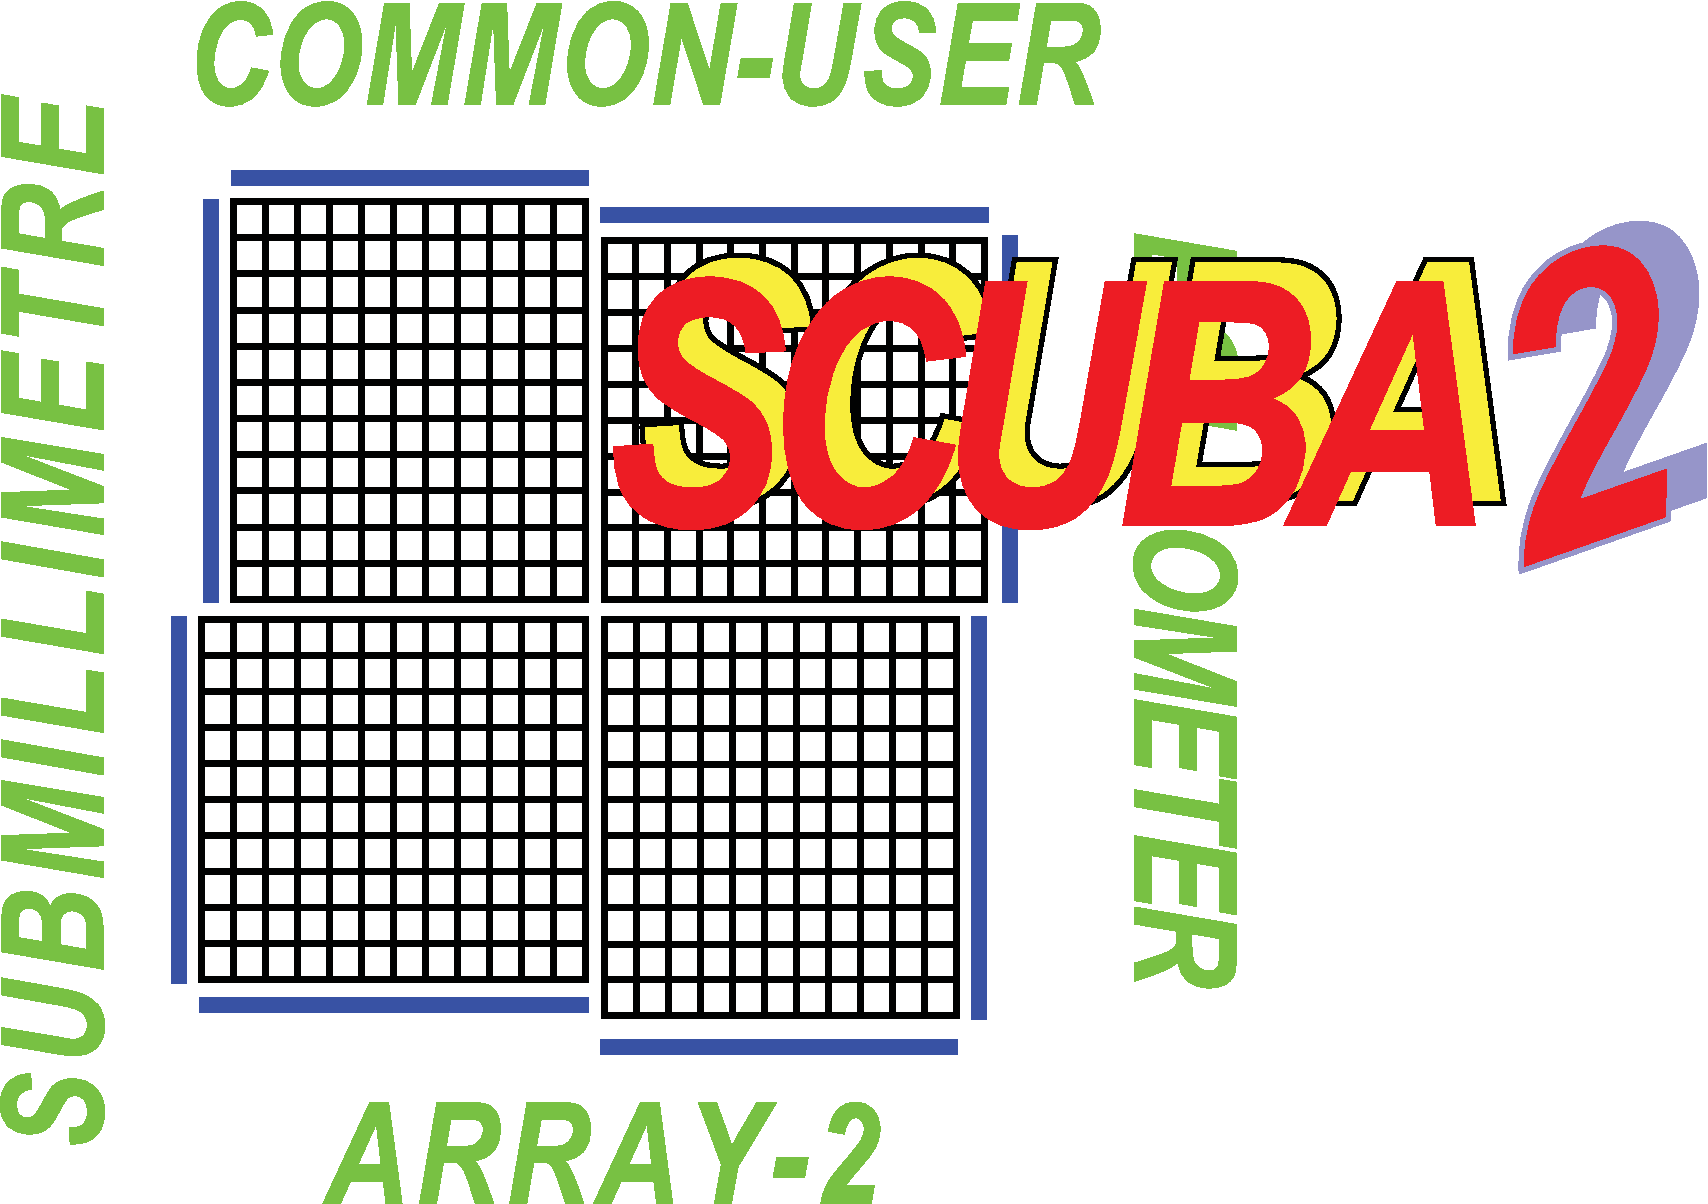
\includegraphics[width=0.7\textwidth]{sc21_s2logo}}


\newcommand{\minipageclear}{%
\begin{minipage}[c]{1.0\linewidth}\end{minipage}}

\begin{document}
\scfrontmatter

% Acronyms section
\Acronyms

\begin{table}[h!]
\begin{tabular}{ll}
\textbf{CADC}   & Canadian Astronomy Data Centre\\
\textbf{CSO}    & Caltech Submillimetre Observatory\\
\textbf{DIMM}   & Dynamic Iterative Map-Maker\\
\textbf{FCF}    & Flux Conversion Factor\\
\textbf{FITS}   & Flexible Image Transport System\\
\textbf{FWHM}   & Full-Width at Half-Maximum\\
\textbf{GAIA}   & Graphical Astronomy and Image Analysis Tool\\
\textbf{ITC}    & Integration Time Calculator\\
\textbf{JCMT}   & James Clerk Maxwell Telescope\\
\textbf{MSB}    & Minimum Schedulable Block\\
\textbf{NDF}    & Extensible N-Dimensional Data Format\\
\textbf{NEP}    & Noise Equivalent Power\\
\textbf{NEFD}   & Noise Equivalent Flux Density\\
\textbf{PSF}    & Point Spread Function\\
\textbf{PWV}    & Precipitable Water Vapour\\
\textbf{RMS}    & Root Mean Square\\
\textbf{SCUBA-2}& Submillimetre Common User Bolometer Array-2\\
\textbf{SMURF}  & Sub-Millimetre User Reduction Facility\\
\textbf{S/N}    & Signal-to-Noise ratio\\
\textbf{SQUID}  & Superconducting QUantum Interference Device\\
\textbf{STC-S}  & Space-Time Coordinate Metadata String Implementation\\
\textbf{SUN}    & Starlink User Note\\
\textbf{TES}    & Transition Edge Sensor\\
\textbf{WVM}    & Water Vapour radioMeter\\
\end{tabular}
\end{table}





\chapter{Introduction}
\label{sec:intro}

% set up page numbers in arabic numerals and restart from 1
\renewcommand{\thepage}{\arabic{page}}
\setcounter{page}{1}

\section{This cookbook}

This guide is designed to instruct SCUBA-2 users on the best ways to
reduce and visualise their data using \starlink\ packages:
\smurf \cite{smurf}, \Kappa \cite{kappa}, \gaia \cite{gaia} and \picard
\cite{picard}.

This guide covers the following topics.
\begin{itemize}
\itemsep0em
\item \cref{Chapter}{sec:intro}{Chapter 1} -- Computer resources you'll need before getting started.
\item \cref{Chapter}{sec:s2}{Chapter 2} -- A description of SCUBA-2 and its observing modes.
\item \cref{Chapter}{sec:raw}{Chapter 3}  -- Data acquisition and instructions for examining raw data.
\item \cref{Chapter}{sec:dimm}{Chapter 4}  -- An introduction to the Dynamic Iterative Map-Maker and a description of the configuration files.
\item \cref{Chapter}{sec:maps}{Chapter 5}  -- How to reduce your data using the map-maker.
\item \cref{Chapter}{sec:postprocess}{Chapter 6}  -- Post-processing reduction steps such as applying the FCF, co-adding multiple maps and estimating the noise.
\item \cref{Chapter}{sec:tweak}{Chapter 7}  -- Options for tailoring the configuration parameters to improve your final map.
\item \cref{Chapter}{sec:eg}{Chapter 8}  -- Two worked examples covering a \htmlref{blank cosmology field}{sec:cosmology} and a \htmlref{galactic field}{sec:bright_ex}.
\item \cref{Chapter}{sec:pipe}{Chapter 9}  -- Instructions for using the \oracdr\ pipeline to reduce your data along with details on data retrieved from the JSA.
\end{itemize}


\section{\xlabel{computing} Before you start: computing resources}

Before reducing SCUBA-2 data using the Dynamic Iterative Map-Maker you should confirm you have sufficient computing resources for your type of map.

We recommend the following:
\begin{table}[h!]
  \centering
  \begin{tabular}{ll}
    \hline
    \textbf{Reduction type} &\textbf{Memory} \\
    \hline
    Large maps (\textsc{pong})& 96 GB\\
    Small maps (\textsc{daisy})&32 - 64 GB\\
    850\,$\mu$m data only&32 - 64 GB\\
    Blank fields&32 - 64 GB\\
    \hline
  \end{tabular}
\end{table}

\subsubsection*{Why these recommendations?}

For large-area maps it is important to process a full observation in a
single chunk. See the text box on
\latexhtml{Page~\pageref{box:chunk}}{\htmlref{Chunking}{box:chunk}}\
for an explanation of chunking. For large maps, using normal map-maker
parameters a machine having 96\,GB is acceptable. It is important that
the memory is as fast as can be afforded, as RAM speed has a direct
linear effect on processing time given that the time-series data are
continually being funnelled through the CPU.

For blank-field surveys, data that only use 850\,$\mu$m, or smaller
regions of the sky you can usefully run the map-maker with less memory
and 32 to 64\,GB is reasonable depending on the specifics of your data
set. \textsc{smurf} is multi-threaded so multiple cores do help
although above eight cores the price/performance gains tend to drop
off.

If you have a very large machine (128\,GB and 24 cores) you can to run
two instances of the map-maker in parallel. Use the
\envvar{SMURF\_THREADS} environment variable to restrict each
map-maker to half the available cores.


\section{\xlabel{software}Before you start: software}

This manual uses software from the \starlink\ packages: \smurf\
\cite{smurf}, \Kappa\ \cite{kappa}, \gaia\ \cite{gaia}, \oracdr\
\cite{oracdr} and \picard\ \cite{picard}. Starlink software must be
installed on your system, and Starlink aliases and environment
variables must be defined before attempting to reduce any SCUBA-2
data.


\subsection{KAPPA and SMURF for data processing}

The Sub-Millimetre User Reduction Facility, or \textsc{Smurf},
contains the Dynamic Iterative Map-Maker, which will process raw
SCUBA-2 data into images (see \smurfsun). \textsc{Kappa} meanwhile is
an application package comprising general-purpose commands mostly for
manipulating and visualising NDF data (see \kappasun). Before starting
any data reduction you will want to initiate both \textsc{Smurf} and
\textsc{Kappa}.

\begin{terminalv}
% smurf
% kappa
\end{terminalv}

You can access the help information by typing \texttt{smurfhelp} or
\texttt{kaphelp} respectively in a terminal, or by using the
\task{showme} facility to access the hypertext documentation. See
\cref{Section}{sec:help}{How to get help} for more information.



\begin{tip}
The .sdf extension on filenames is not required when running
Starlink commands.
\end{tip}


\subsection{GAIA for viewing your map}

Image visualisation can be done with \gaia\ (see
\gaiasun). \textsc{Gaia} is an image and data-cube display and
analysis tool, which incorporates facilities such as source detection,
three-dimensional visualisation, photometry and the ability to query
and overlay on-line or local catalogues.
\begin{terminalv}
% gaia map.sdf
\end{terminalv}

\subsection{ORAC-DR for running the pipeline}

The \oracdr\ Data Reduction Pipeline \cite{oracdr} (hereafter just
\textsc{Orac-dr}) is an automated reduction pipeline. \textsc{Orac-dr}
uses \smurf\ and \Kappa\ (along with other Starlink tools) to perform
an automated reduction of the raw data following pre-defined recipes
to produce calibrated maps.  The following commands initialise
\textsc{Orac-dr} ready to process 850\,$\mu$m and 450\,$\mu$m data
respectively.
\begin{terminalv}
% oracdr_scuba2_850
% oracdr_scuba2_450
\end{terminalv}
For more information on available recipes and intructions for running the pipeline
see \cref{Chapter}{sec:pipe}{The SCUBA-2 Pipeline}.

\subsection{PICARD for post-reduction processing}

\textsc{Picard} uses a similar pipeline system as \oracdr\ for
post-processing analysis of reduced data. \textsc{Picard}
documentation can be found at
\href{http://www.oracdr.org/oracdr/PICARD}{\textsc{Orac-dr} web page},
or at \picardsun. All \textsc{Picard} recipes follow the same
structure and are run like so:
\begin{terminalv}
% picard -recpars <recipe_params_file> RECIPE <input_files>
\end{terminalv}
where \param{<recipe\_param\_file>} is a text file containing the
relevant recipe parameters. \param{RECIPE} is the name of the recipe
to be run (note the caps). The list of files to be processed is given
by  \param{<input\_files>}. These must be in the current directory or a
directory defined by the environment variable \envvar{ORAC\_DATA\_IN}. A
number of \textsc{Picard} recipes will be demonstrated in
\cref{Chapter}{sec:maps}{Reducing your data}.

Other command-line options include \texttt{-log xsf} where the log
file is written to any combination of the screen [\texttt{s}], a file
[\texttt{f}] or an X-window [\texttt{x}]. \texttt{s} or \texttt{sf} is
recommended as the recipes are short and the X-window automatically
closes upon completion.

You do not specify an output filename for \picard, instead the output
is generated by adding a recipe depending suffix to the input
filename. If there is more than one input file then the name of the
last file is used.

You can create a file which lists the input files to be passed to
\picard\ for processing. this file is read by \picard\ via the
Linux/Unix \task{cat} command. For example:

\begin{terminalv}
% picard -log s RECIPE_NAME `cat myfilestoprocess.lis`
\end{terminalv}

To execute the \task{cat} command you must enclose it in back
quotes. You must also include the \file{.sdf} extension on any files
passed to \picard.

\begin{tip}
  The .sdf extension on filenames is required by \textsc{Picard}.
\end{tip}

\begin{tip}
  If the environment variable \envvar{ORAC\_DATA\_OUT} is defined, any
  files created by \textsc{Picard} will be written in that
  location. Check there if new files are expected but do not appear in
  your working directory.
\end{tip}


\subsection{\xlabel{help}How to get help}
\label{sec:help}

\begin{table}[h!]
\begin{tabular}{p{2.3cm}|p{7.3cm}|p{5cm}}
\hline
\textbf{Help\newline command} & \textbf{Description} & \textbf{Usage}\\
\hline
\task{showme} & If you know the name of the Starlink document you want to view
                use \task{showme}. When run, it launches a new webpage or tab
                displaying the hypertext version of the document. &
                \begin{terminalv}
% showme sun95
\end{terminalv}
\\
\hline
\task{findme} & \task{findme} searches Starlink documents for a keyword. When
                run, it launches a new webpage or tab listing the results. &
                \texttt{\% findme kappa}\\
\hline
\task{docfind} & \task{docfind} searches the internal list files for keywords. It then
                 searches the document titles. The result is displayed using the
                 Unix \task{more} command. & \texttt{\% docfind kappa}\\
\hline
Run routines with prompts & You can run any routine with the option
                            \texttt{prompt} after the command. This will
                            prompt for every parameter available. If you
                            then want a further description of any parameter
                            type  \texttt{?} at the relevant prompt. &
                            \texttt{\% makemap prompt \newline\ \% REF - Ref. NDF /!/$>$ ?}\\
\hline
\end{tabular}
\end{table}

\section{Processing options}

You have two options for processing your data:

\begin{enumerate}
\item performing each step manually, or
\item running the automated pipeline (\textsc{Orac-dr}).
\end{enumerate}

The pipeline approach works well if you have a lot of data to process.
Performing each step by hand allows more fine-tuned control of certain
processing and analysis steps, and is especially useful for refining
the parameters used by the map-maker. However, once the optimal
parameters have been determined, it is possible to pass them to the
pipeline. \cref{Chapter}{sec:dimm}{The Dynamic Iterative Map-maker
  Explained} and \cref{Chapter}{sec:maps}{Reducing Your Data} discuss
the manual approach; to use the science pipeline, skip straight to
\cref{Section}{sec:pipe}{The SCUBA-2 Pipeline}.

The JCMT will produce pipeline reduced files for each observation and
group of repeat observations for each night. These are reduced using
the \oracdr\ pipeline with the recipe specified in the MSB.
\cref{Chapter}{sec:pipe}{The SCUBA-2 Pipeline} gives instruction on
retrieving reduced data from the \htmladdnormallink{JCMT Science
  Archive}{http://www3.cadc-ccda.hia-iha.nrc-cnrc.gc.ca/jcmt/} at
CADC.



\chapter{\xlabel{scuba2_overview}SCUBA-2 Overview}
\label{sec:s2}
\section{\xlabel{scuba2}The instrument}


The Submillimetre Common User Bolometer Array-2 (SCUBA-2) is a
10,000-pixel bolometer camera. It has two arrays operating
simultaneously to map the sky in the atmospheric windows of 450 and
850$\mu$m.

\subsubsection*{How it works}
The SCUBA-2 bolometers are integrated arrays of superconducting
transition edge sensors (TESs) with a characteristic transition
temperature, $T_c$. In addition, each TES is ringed with a resistive
heater which can compensate for changes in sky power. The SCUBA-2
focal plane is kept at a base temperature slightly below $T_c$,
however a voltage is applied across each TES resistance to position
the bolometer at the transition temperature. From this point, any
increase of temperature on the bolometers (e.g. from an astronomical
signal) will increase the TES resistance and heat it up. This causes a
drop in current and therefore a drop in temperature making the system
self-regulating.

For properly performing bolometers, the change in current through the
TES is proportional to the change in resistance, with the response
calibrated using flat-field observations (described below). This
changing current generates a magnetic field which is amplified by a
chain of superconducting quantum interference devices (SQUIDs). This
induces a feedback current which is proportional to the current
flowing through the TES, and it is this feedback current that is
recorded during data acquisition.


\subsubsection*{Setups}

Before science data can be taken the system must be optimised. These
`setups' are performed after slewing to the azimuth of the source,
where the SQUID, TES and heater biases are set to pre-determined
nominal values, in order to position the bolometers in the middle of
the transition range.

\subsubsection*{Flat-field}

 The shutter then opens onto the sky, and
as it does so the gradual increase in sky power hitting the array is
compensated for by a decrease in the resistive heater power via a
servo loop designed to keep the TES output constant. This acts to keep
the bolometers positioned at the centre of the transition range and is
known as \textbf{heater tracking}.

The responsivity of the bolometers will change slightly between the
dark and the sky; therefore, once the shutter is fully open a fast
\textbf{flat-field} observation is carried out to recalibrate them.
\textbf{A flat-field measures the responsivity of each bolometer to
changing sky power}. It does this by utilising the resistance heaters
which are ramped up and down around the nominal value. The change in
current through the TES is then recorded for each bolometer giving a
measure of its responsivity. The flat field solution is then the
inverse linear gradient of the current as a function of heater power.

At this point bolometers with responsivities above or below a
threshold limit are rejected, along with bolometers that display a
non-linear response or have a poor S/N. A second flat-field is
performed at the end of an observation so bolometers whose
responsivity has changed over the course of the observation can be
flagged.

For full details of the array setup and operation see Holland et al.
(2013) \cite{s2main}.

\begin{figure}[t!]
\begin{center}
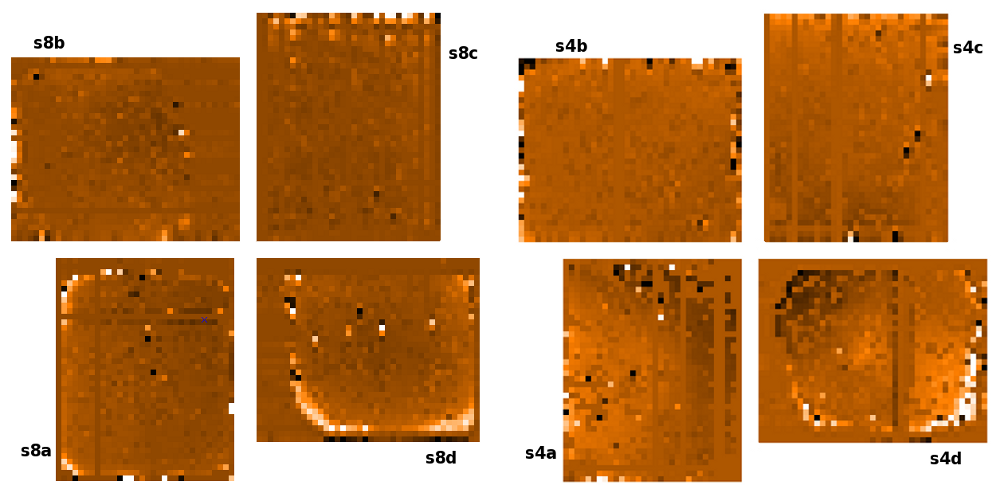
\includegraphics[width=0.8\linewidth]{sc21_arrays}
\label{fig:arrays}
\caption[The physical layout of the arrays at each wavelength]{
  \small The layout of the arrays at 850$\mu$m (left) and
  450$\mu$m (right). The labels denote the name assigned to each
  sub-array. Raw data files are generated separately for each sub-array
  and must be co-added. This figure was made by running
 \wcsmosaic\ on a raw sub-scan from each sub-array.
}
\end{center}
\end{figure}

\section{\xlabel{obs_modes}Observing modes}
\label{sec:mmodes}

Two observing modes are offered for SCUBA-2---\textsc{daisy} and
\textsc{pong}. As the bulk of \mbox{SCUBA-2} observing involves
large area mapping, both observing modes are scan patterns. Your
choice depends on the size of the area you wish to map, where you
would like your integration time concentrated and the degree of
extended emission you wish to recover.


\begin{aligndesc}

\item[\textbf{PONG}] A \textsc{pong} map is the scan strategy for
  covering a large area. The default options allow for three
  sizes---900\,arcsec, 1800\,arcsec and 3600\,arcsec. A single
  \textsc{pong} map is a square of these dimensions and the telescope
  fills in the square by bouncing off the edge of the area. To ensure
  an even sky background it is recommended a minimum of three, but
  preferably more than five, \textsc{pong} maps are included in a
  single observation with a rotation introduced between each one. In
  this way a circular pattern is built up, (see the lower right-hand
  panel of \cref{Figure}{fig:scan}{graphic below}), with a diameter
  equal to your requested map size.

  To recover large-scale extended structure you are advised to use
  larger \textsc{pong} maps which scan at a higher rate. This option
  is preferable to tiling multiple smaller maps. Ultimately it is the
  size of the SCUBA-2 field-of-view that determines the sensitivity to
  large-scale structure.

\item[\textbf{DAISY}] \textsc{daisy} maps are the option for
  point-like or compact sources ($<$3~arcmin) by maximising the
  exposure time on the centre of the image. The telescope moves at a
  constant velocity in a `spirograph' pattern that has the advantage
  of keeping the source on the array throughout the observation. This
  is shown in the top panel of \cref{Figure}{fig:scan}{the figure
    below}.

\end{aligndesc}

\subsubsection*{Why these patterns?}

SCUBA-2 removes atmospheric noise in the data-processing
stage (Holland et al. 2013) \cite{s2main}. The power spectrum
of data taken by SCUBA-2 has a $1/f$ noise curve at lower frequencies. To
ensure astronomical signals are far away from this $1/f$ noise, fast
scanning speeds are required.

In order to disentangle source structure from other
slowly varying signals (e.g. extinction, sky noise, $1/f$ noise), the
scan pattern must pass across each region of the map from different
directions and at different times. The scan patterns themselves, along
with the associated parameters (velocity and scan-spacing), have been
designed and optimised to meet both these criteria.

\starfig{sc21_wayne_scan}{[t!]}{width=0.98\linewidth}{fig:scan}{%
  Illustration of the SCUBA-2 observing patterns}{%
  From left: telescope track over a single rotation of the pattern;
  telescope track after multiple rotations of the pattern; resulting
  exposure time map. The scan pattern for your observation can be
  visualised in this way with \topcat\ using the output from
  \jcmtstate.  See \cref{section}{sec:scan}{Displaying scan patterns} for
  more details.  Figure modified from Holland et al. (2013).
}

\chapter{\xlabel{data_files}Handling Raw SCUBA-2 Data}
\label{sec:raw}

This chapter describes a number of procedures visualising and
assessing the quality of raw data files.  These steps need not be part
of your data reduction process and do not concern the iterative
map-maker.

However, there are reasons you may wish to examine your raw data in
greater depth. The most likely motivation is unusual result from the
map-maker such as higher than expected noise, artefacts in your map,
or inconsistent noise across multiple tiles.  This chapter will help
you get to the bottom of many of these issues.

\section{Data acquisition explained}
A normal science observation will follow the following sequence.

\begin{enumerate}\itemsep-0.2em
\item Flat-field
\item Science scans
\item Flat-field
\end{enumerate}

The \param{SEQ\_TYPE} keyword in the FITS header may be used to
identify the nature of each scan (see
\cref{Section}{sec:fitsheader}{Headers and file structure}).  When you
access raw from the \htmladdnormallink{Science
  Archive}{http://www3.cadc-ccda.hia-iha.nrc-cnrc.gc.ca/jcmt/} you
will get all of the files listed above. Later when you reduce your
data using the map-maker you must include all the science files
\emph{and} the first flat-field.  The final flat-field is not
currently used.

Shown below is a list of the raw files for a single sub-array (in this
case s8a) for a short calibration observation. The first and last
scans are the flat-field observations,which occur after the shutter
opens to the sky at the start of the observation and closes at the end
(note the identical file size); all of the scans in between are
science.


\begin{terminalv}
% ls -lh /jcmtdata/raw/scuba2/s8a/20131227/00034
\end{terminalv}

\begin{terminalv}
-rw-r--r-- 1 jcmtarch jcmt 8.0M Dec 27 03:00 s8a20131227_00034_0001.sdf
-rw-r--r-- 1 jcmtarch jcmt  22M Dec 27 03:00 s8a20131227_00034_0002.sdf
-rw-r--r-- 1 jcmtarch jcmt  22M Dec 27 03:01 s8a20131227_00034_0003.sdf
-rw-r--r-- 1 jcmtarch jcmt  22M Dec 27 03:02 s8a20131227_00034_0004.sdf
-rw-r--r-- 1 jcmtarch jcmt  22M Dec 27 03:02 s8a20131227_00034_0005.sdf
-rw-r--r-- 1 jcmtarch jcmt 6.8M Dec 27 03:02 s8a20131227_00034_0006.sdf
-rw-r--r-- 1 jcmtarch jcmt 8.0M Dec 27 03:03 s8a20131227_00034_0007.sdf
\end{terminalv}

The SCUBA-2 data acquisition (DA) system writes out a data file every
30 seconds; each of which contains 22\,MB of data. The only exception
is the final science scan which will usually be smaller (6.8\,MB in
the example above), typically requiring less than 30 seconds of data
to complete the observation.

\textbf{Note:} All of these files are written out eight times, once
for each of the eight sub-arrays.

The main data arrays of each file are cubes, with the first two
dimensions enumerating columns and rows, and the third time slices
(sampled at 200\,Hz).

\subsubsection*{Units}

Raw SCUBA-2 data come in uncalibrated units. The first calibration
step is to scale the raw data to units proportional to picowatts (pW)
by applying the flat-field solution. This step is performed internally
by the map-maker but can be done manually when examining the raw
data---see \cref{Section}{sec:concat}{Concatenate \& apply a
  flat-field}.

The second step is to scale the data by the flux conversion factor
(FCF) to give units of janskys. Unless you are running the
\textsc{Orac-dr} pipeline, this must be done manually with the
instructions given in \cref{Section}{sec:cmult}{Flux conversion
  factors}.


\section{\xlabel{concat}Concatenate \& apply a flat-field}
\label{sec:concat}

Since SCUBA-2 data for a given sub-array are broken into multiple
30-second scans by the data acquisition (DA) system, it is useful to
concatenate the data into a single file. The \smurf\ task \concat\ can
be used for this operation. The example below combines all of the
files associated with Observation 8 for the s8a array into a single
file called \file{s8a20120725\_0008\_con}.

\begin{terminalv}
% sc2concat s8a20120725_0008\*.sdf s8a20120725_0008_con
\end{terminalv}

\task{sc2concat} will automatically filter out any dark or flat-field
observations, so that the concatenated file contains only the science
data. Be careful when concatenating a very long observation since the
output file may be too large to reasonably handle. Fifteen-minute
chunks (30 files) should be sufficient.

\task{sc2concat} applies the flat-field by default (although it can be
disabled using the \param{noflat} option on the command-line).

The flat-field can also be applied manually using the \flatfield\
command.

\begin{terminalv}
% flatfield 's8a20120701_0008*.sdf' '*_flat'
\end{terminalv}
Here, the output will be a flat-fielded version of each science scan
in Observation 8; the file names will be the original input
names with \_flat appended to them.

As a rule of thumb, you should apply the flat-field to your data
before examining it.


\begin{tip}
You do not need to apply the flat-field prior to reducing your
data with the map-maker.
\end{tip}

\section{\xlabel{header}Headers and file structure}
\label{sec:fitsheader}

There are two \Kappa\ tasks which are extremely useful for examining
your data: \fitslist\ and \ndftrace, which can be used to view the
FITS headers and dimensions of the data.


\begin{aligndesc}
\item[\textbf{\task{fitslist}:}] This lists the FITS header
  information for any file (raw or reduced). This extensive list
  includes dates \& times, source name, scan type, pattern and
  velocity, size of the map, exposure time, start and end elevation,
  opacity, and the temperature of the instrument. An example is given
  below:
\begin{terminalv}
% fitslist s8a20120720_00030_000\*.sdf | grep SEQ_TYPE
\end{terminalv}

If you already know the name of the parameter you want to view you can
use the \fitsval\ command instead, e.g.%\\
\begin{terminalv}
% fitsval file.sdf TAU225ST
\end{terminalv}

\item[\textbf{\task{ndftrace}:}] \task{ndftrace} displays the
  attributes of the data structure. This will tell you the units of
  the data, pixel bounds, dimensions, world coordinate bounds and
  attributes, and axis assignations.
\begin{terminalv}
% ndftrace file.sdf fullframe
\end{terminalv}

\end{aligndesc}


Full details of these commands can be found in the
\xref{\textsc{Kappa} manual}{sun95}{}.

\begin{figure}[ht!]
\begin{center}
\begin{fmpage}{0.95\linewidth}
\textbf{Topcat Example}
\minipageclear
\vspace{0.5cm}

\begin{minipage}[c]{0.6\linewidth}

\begin{terminalv}
% topcat -f tst 20120720_30.tst
\end{terminalv}
\end{minipage}
\hspace{0.3cm}
\begin{minipage}[c]{0.32\linewidth}
Load the tst file generated by \task{jcmtstate2cat} into \topcat.
\end{minipage}
\minipageclear

\vspace{0.5cm}

\begin{minipage}[c]{0.6\linewidth}
\begin{center}
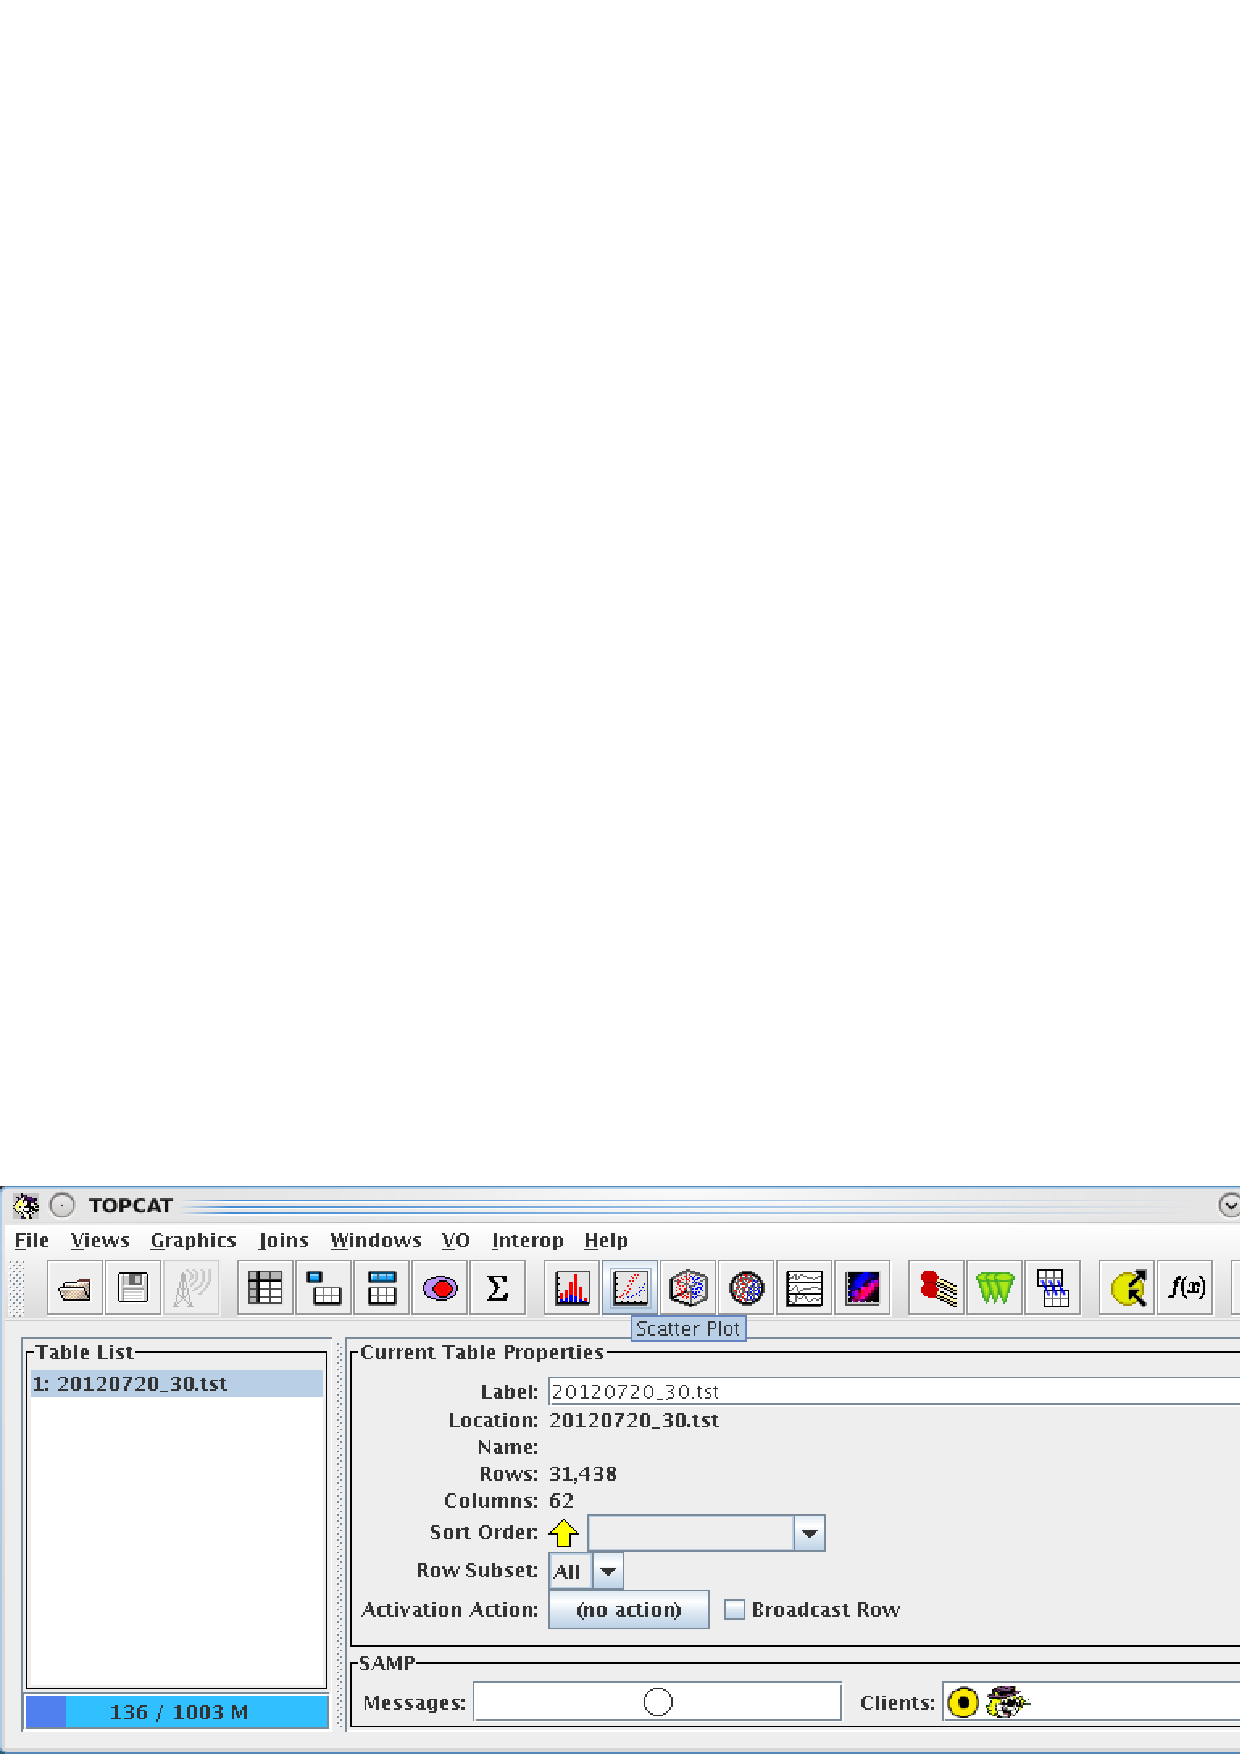
\includegraphics[width=0.95\textwidth]{sc21_topcat1}
\end{center}
\end{minipage}
\hspace{0.3cm}
\begin{minipage}[c]{0.32\linewidth}
In \topcat\ select the scatter plot option
from the menu bar across the top of the window.
\end{minipage}
\minipageclear
\vspace{0.5cm}

\begin{minipage}[c]{0.6\linewidth}
\begin{center}
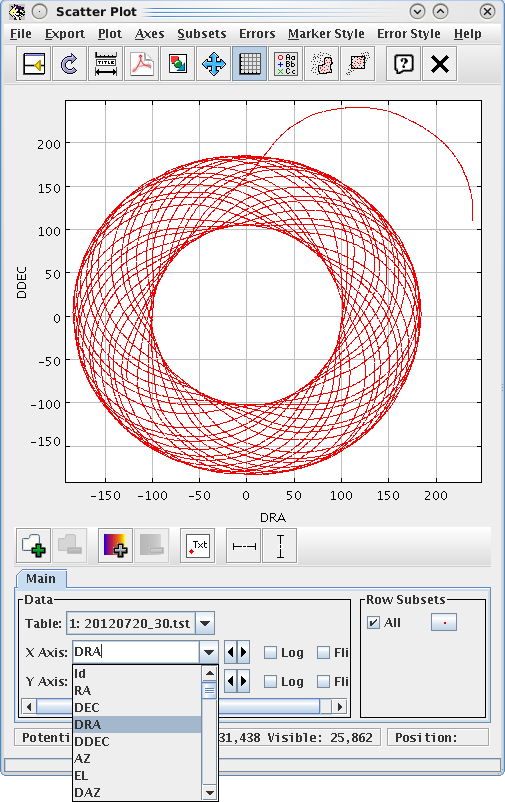
\includegraphics[width=0.75\textwidth]{sc21_topcat2}
\end{center}
\vspace{0.2cm}
\end{minipage}
\hspace{0.3cm}
\begin{minipage}[c]{0.32\linewidth}
With the scatter plot displayed you can adjust the $X$-axis and
$Y$-axis values to DRA and DDEC respectively to display the scan pattern.
If you are interested in seeing how any of the variables change over time,
select the the $X$ Axis to be either Id or RTS\_NUM.
\end{minipage}
\minipageclear

\end{fmpage}
\end{center}
\caption[Displaying the scan pattern with \topcat] { \small \topcat\
  example demonstrating how to display the scan pattern for an
  observation.  }
\label{fig:topcat}
\end{figure}


\section{\xlabel{scan_pat}Displaying scan patterns}
\label{sec:scan}

The movement of the telescope throughout a scan (as well as other
state information) is stored in the \texttt{MORE.SMURF.JCMTSTATE}
extension of a data file. The \smurf\ task \jcmtstate\ converts this
information into a simple ASCII tab-separated table.

\begin{terminalv}
% jcmtstate2cat s8a20120701_00008_*.sdf > state.tst
\end{terminalv}

Multiple files can be supplied to the command using standard shell
wild cards. If you have already concatenated your data you can simply
input the single concatenated file. It may be useful to view the scan
pattern for your observation, particularly for maps taken at high
elevations, to ensure the pattern completed successfully.


\begin{tip}
  Follow the \task{jcmtstate} command with \texttt{-h} to find out
  more information.
\end{tip}


This catalogue can be loaded into \topcat\ for plotting, making sure
to specify the TST format during loading.

\begin{terminalv}
% topcat -f tst state.tst
\end{terminalv}

Example of scan patterns displayed with \topcat\ can be seen in
\cref{Figure}{fig:scan}{telescope tracks}. Detailed instructions on
how to display the scan pattern for your observation are given in
\cref{Figure}{fig:topcat}{box below}.  All of the time-varying header
values are available for plotting. Other values include the azimuth
and elevation offsets (DAZ \& DEL), the WVM and 225\,GHz opacity
values, and the instrument temperatures (e.g.  SC2\_FPUTEMP gives the
temperature of the focal plane).

Due to extreme accelerations at ``turn-around'' points of a scan
pattern (especially for \textsc{pong}s), the telescope finds it hard
to follow the proscribed scan patterns at high elevations. To mitigate
this we try to avoid observing any sources above 70$^\circ$ elevation.
If the \fitslist\ keywords \param{ELSTART} and \param{ELEND}
indicate that your map was taken at high elevation you may consider
checking the success of the scan pattern. If you find your observation
has failed to follow the demanded scan pattern don't worry, the data are
likely to still be useful. This is especially true for \textsc{daisy}
maps where the high exposure-time central region is usually
unaffected.

\section{\xlabel{display_cube}Displaying time-series data}
\label{sec:gaiacube}

Use the \starlink\ application \textsc{Gaia} to visualise the
bolometer time-series data (or indeed \emph{any} SCUBA-2 data
file). This is initiated simply typing \texttt{gaia} into a terminal.

\begin{terminalv}
% gaia s8a20120725_00058_con.sdf
\end{terminalv}

Loading a file in \textsc{Gaia} produces two windows. The main window
(see \cref{Figure}{fig:gaia_main}{upper graphic}) shows a map of
bolometer values at a given point in time. The time slice displayed
may be changed by scrolling through the time axis. This is done in the
second window entitled \gaiathing{Display image sections of a
  cube}. The \gaiathing{Index of plane} slider towards the top of this
window may be moved to display different time slices in the main
window.

\starfig{sc21_gaia1}{[b]}{width=\linewidth}{fig:gaia_main}{
  Raw data displayed in the main \gaia\ window}{
  Initial \gaia\ windows displayed upon loading a data cube.
  The main window in the left shows a map of bolometer values at a fixed
  sample in time. You may have to zoom in multiple times by clicking the
  \gaiathing{Z} icon. On the right-hand side, the
  \gaiathing{Display image sections of a cube}
  dialogue enables you to navigate the time axis.
}

A third window will appear when you click on a bolometer---the
\gaiathing{Spectral plot} (see \cref{Figure}{fig:gaia_spec}{lower graphic}).
This shows an automatically scaled plot of the raw time stream of data for
that given bolometer. It will be overridden when you click on a different
bolometer.

\starfig{sc21_gaia2}{[t]}{width=0.8\linewidth}{fig:gaia_spec}{ \gaia\
  spectral plot window}{ The \gaiathing{Spectral plot} window displays
  the time-varying signal. This window appears automatically when a
  bolometer is clicked in the main window.  The vertical red line
  indicates the time slice that is currently selected in the
  \gaiathing{Display image sections of a cube} dialogue---this can be
  dragged across the spectrum to scroll through the time-slices.  }

A second way to scroll through the time axis is to click and drag the
vertical red bar on the \gaiathing{Spectral plot} window. As you do
so, the array shown in the main window will automatically update.

To highlight small variations between bolometers you will need to
change the auto cut and (depending on your preference) the colour
scheme---both are controlled by buttons on the sidebar.

See the \xref{\textsc{Gaia} manual}{sun214}{} for full
details.\footnote{\url{http://docs.jach.hawaii.edu/star/sun214.htx/sun214.html}}


\section{\xlabel{regrid_map}Regridding data into a map}
\label{sec:regrid}

Any raw time-series data can be quickly regridded into sky frame
coordinates using the \smurf\ \makemap\ task in rebin mode. This
involves no processing of the data. The following command produces a
map from the raw concatenated data; unlike the iterative mode of
\task{makemap} described in the next chapter, no configuration file is
required.

\begin{terminalv}
% makemap s8a20120725_00058_con.sdf crl2688_sky method=rebin
\end{terminalv}

The output map here is called \file{crl2688\_sky.sdf} and is shown in
\cref{Figure}{fig:regrid}{the figure below}.  The pixel scale is left
at the default values of 2\,arcsec on a side at 450$\mu$m and
4\,arcsec at 850$\mu$m (although this can be changed using the
\texttt{pixsize=}$x$ option on the command-line, where $x$ is in
arcsec).

\starfig{sc21_crl2688_regrid}{[b!]}{width=0.65\linewidth}{fig:regrid}{
  The regridded map of CRL~2688 displayed with \gaia.}{ The regridded
  map of CRL~2688 with the s8a sub-array displayed with \gaia.  }

\begin{tip}
  If you do not include \param{method=rebin}, the map-maker will will
  default to \param{method=iterate}.
\end{tip}


\section{\xlabel{clean}Notes on cleaning your data}
\label{sec:clean}

Cleaning raw data is an essential first step towards making a quality
final map. The map-maker performs all of these cleaning steps during
the pre-processing stage. The commands for manually cleaning your data
are given in \cref{Appendix}{app:clean}{Cleaning the raw data}.  You
can also check out the SMURF SRO
Cookbook{\footnote{\url{http://www.starlink.ac.uk/docs/sc19.htx/sc19.html}}}
which goes into great depth on the data cleaning options.


\section{\xlabel{calcnoise}Checking the array performance}
\label{sec:calcnoise}

The on-sky performance of the array can be assessed using the \smurf\
command \calcnoise. Rather than give an absolute measure,
\task{calcnoise} should be used as an indicator of array performance
and stability.  \task{calcnoise} cleans the data then calculates the
white noise on the array (between 2 and 10\,Hz by default).
\begin{terminalv}
% calcnoise s8a20110720_00030\*.sdf s8a_noise power=!
\end{terminalv}
It will prompt for a configuration file to describe the cleaning
steps. The default is the supplied \file{dimmconfig\_calcnoise.lis}.
Two noise measurements are reported in the terminal: the `Effective
noise' and the `Effective NEP'.

An output file is created for each sub-array with the NEP map stored
in the \texttt{.MORE.SMURF.NEP} extension.

If you have a bright source in the field this will contaminate the
signal. In this case you should examine the \model{NOI} model from the
map-maker instead---see \cref{Section}{sec:models}{The individual
  models} for a description and \cref{Section}{sec:export}{Exporting
  individual models} for details on how to examine it.

\chapter{\xlabel{dimm}The Dynamic Iterative Map-Maker Explained}
\label{sec:dimm}

The Dynamic Iterative Map-Maker, hereafter just referred to as the
map-maker is the tool you will use to produce SCUBA-2 maps. It
performs all pre-processing steps to clean the data, followed by
iteratively solving for multiple signal components and regridding to
produce a final science map.

This chapter describes how the map-maker produces a science images
from raw SCUBA-2 data. It is essential reading to gain an
understanding of what has happened to produce your reduced image,
especially if you wish to modify the default map-maker parameters.
\color{red} If you prefer to jump straight in to the data reduction go
to \cref{Chapter}{sec:maps}{Reducing Your Data}.\color{black}


\section{\xlabel{dimm_theory}How it works}

The map-maker works by individually modelling the various
contributions that make up the signal recorded by each bolometer. It
models and then subtracts all the sources of signal in order of
decreasing magnitude, ultimately leaving just the astronomical signal
plus noise. A list of the modelled components can be seen in
\cref{Table}{tab:mods}{tabulated} and a description found in
\cref{Section}{sec:models}{The individual models}.

\textbf{The map-maker requires a configuration file to accompany each
  reduction.} This file instructs the map-maker on the pre-processing
steps, which components to iteratively model, the parameters to use
when doing so, and the stopping (or convergence) criteria.  There is a
single generic default configuration file called
\file{dimmconfig.lis}.  Its configuration parameters are tabulated in
\cref{Appendix}{app:dimm}{an appendix}.

Often, the default configuration file will not give optimal results
for your particular observation. For this reason, specialised
configuration files have been developed which are tailored to
different science goals, be they detecting faint galaxies or mapping
large molecular clouds. A description of these specialised
configuration files can be found \cref{in Section}{sec:config}{here}
with listings \cref{in Appendix}{app:special}{this appendix}.


\section{The reduction step-by-step}

\textbf{This description applies to the default configuration file ---
  \file{dimmconfig.lis}.}

\cref{Figure}{fig:dimm}{The graphic below} shows the flow chart of the
map-making process for \file{dimmconfig.lis}. It is divided into two
sections: the pre-processing stage where the data are cleaned, then
the iterative stage where the different models are subtracted, a sky
map created and the convergence checked.



\begin{enumdesc}
\item[Initial cleaning and downsampling]

  The first task of the map-maker is to down-sample the data. The raw
  time-series data are re-sampled at a rate that matches the requested
  pixel size, the equivalent to applying a low-pass filter.
  Down-sampling saves time and memory usage when running the
  map-maker.  The raw data are then concatenated and have the
  flat-field (from the bracketing fast flat scans) applied to
  calibrate the bolometers. A number of cleaning steps are then run: a
  polynomial baseline is subtracted from each bolometer; spikes and DC
  steps are removed; and any resulting gaps in the time-series are
  filled in.

\item[Iterative steps]

  Next comes the iterative stage. First to be modelled and removed are
  \model{COM} and \model{GAI}, which work together to calculate the
  average signal template of all the bolometers, and then fit/remove
  the templates from each bolometer. The next model (\model{EXT})
  applies a multiplicative extinction correction to the
  data. Following this, a Fourier transform is applied to the data and
  the \model{FLT} model is removed in the frequency domain.
  \model{FLT} applies a high-pass filter to the data, above
  frequencies that correspond to angular scales of 600\,arcsec and
  300\,arcsec at 450$\mu$m and 850$\mu$m, respectively.


  The first step in creating the \model{AST} model involves regridding
  the data to produce an estimation of the final science map.  Since
  many samples typically contribute to the estimate of the signal in a
  given pixel, the noise is greatly reduced compared with the
  time-series data. This map is then projected back into the time
  series and the \model{AST} model removed. The \model{NOI} model then
  measures the noise in the residual signals for each bolometer to
  establish weights for the data as they are placed into the map in
  subsequent iterations.


\item[Checking convergence]

  Convergence is checked against the parameters detailed in the
  configuration file. Convergence is achieved either when the
  requested number of iterations has been completed, or when the
  noise-based convergence criterion specified in the configuration
  file is reached. If more iterations are required or (in the latter
  case) the residual noise has not converged then \model{GAI},
  \model{EXT}, \model{FLT} and \model{COM} models are all undone and
  the time-series is reconstructed. The sequence is then rerun only
  this time without \model{AST} complicating the model fitting.
\end{enumdesc}


\starfig{sc21_flow_dimm_blue}{}{width=0.78\linewidth}{fig:dimm}{
  Flowchart of the map-maker}{ A flow chart illustrating the dynamic
  iterative map-maker. Note that for each iteration the \model{AST}
  model is subtracted from the time-series leaving only those
  contributions to be fitted and removed.  }

For full details of the map-maker see \textbf{Chapin et al. (2013)}
\cite{mapmaker}.

\setlength{\extrarowheight}{3pt}
\begin{table}
\centering
\begin{tabular}{c|l}
\hline
\textbf{Model} &\hspace{0.2cm} \textbf{Description} \\
\hline
\model{COM}&\hspace{0.2cm} Common-mode signal\\
\model{GAI}&\hspace{0.2cm} Common-mode scaled to each bolometer---the gain\\
\model{EXT}&\hspace{0.2cm} Extinction correction\\
\model{FLT}&\hspace{0.2cm} Fourier transform filter\\
\model{AST}&\hspace{0.2cm} Map estimate of astronomical signal\\
\model{NOI}&\hspace{0.2cm} Noise estimation\\
\hline
\end{tabular}
\label{tab:mods}
\caption{\small Table adopted from Chapin et al. (2013). A detailed
explanation of each model is given in \cref{Section}{sec:models}{The individual models}.}
\end{table}

\raggedbottom
\section{\xlabel{models}The individual models}
\label{sec:models}

The particular sequence of the models evaluated (and removed) by the
map-maker during the iterative stage is indicated by the
\texttt{modelorder} parameter in the configuration file. These models
are modular however, so their order may be changed. The default model
order in \file{dimmconfig.lis} is given below.


\begin{terminalv}
modelorder = (com,gai,ext,flt,ast,noi)
\end{terminalv}


The only recipe not following this model order is the one tailored for
blank field maps which does not include a \model{FLT} model in the
iterative stage (see \cref{Section}{sec:config}{Specialised
  configuration files}).

Below is an introduction to each model. More complete descriptions of
the models and all the associated caveats can be found in Chapin et
al.  (2013) \cite{mapmaker}.

\begin{longtable}{c p{0.8\textwidth}}
  \hline
  \textbf{MODEL} & \multicolumn{1}{c}{\textbf{DESCRIPTION}}\\
  \hline
  \endhead
  \ifpdf
  \hline
  \endfoot
\fi
  COM& The \model{COM} model removes the common-mode signal
  (the signal that is common to all bolometers), the dominant
  contributor to this signal being the sky noise. It determines this
  by simply averaging over all bolometers for each time slice.
  Bolometers are flagged as bad, (and thus omitted from the final
  map), if they do not resemble the \model{COM} model seen by the
  majority of the other bolometers.

  Extended emission on a scale larger than the array footprint on the
  sky will contribute a signal indistinguishable from a common-mode
  signal. This puts an upper limit on the spatial scale of
  astronomical emission that can be recovered.\\
  \hline
GAI& \model{GAI} model works with \model{COM} in removing the
  common-mode signal. \model{GAI} is used to scale the \model{COM}
  model that has been subtracted and is described by a gain and an
  offset to scale all the bolometers to the same level. This will
  allow the bolometers to share a common calibration further down the
  line.\\
\hline
EXT& \model{EXT} applies the extinction correction. This is a
  time-varying scaling factor that is derived from the JCMT
  water-vapour radiometer. As it deals with 30-second chunks of data,
  this accounts for varying conditions over a long observation. For
  more details see \cref{Appendix}{app:cal}{SCUBA-2 data
    calibration}.\\
\hline
FLT& The \model{FLT} model acts on the Fourier transform of the
  bolometer data. High-pass (only allows \textit{higher} frequencies
  to pass) and low-pass (only allows \textit{lower} frequencies to
  pass) filters can be specified. These cut-off frequencies can either
  be be specified by you directly or as an angular spatial scale
  (which is subsequently) converted into a frequency dependent on the
  speed at which the telescope is moving). The most important role of
  this model is to apply a high-pass filter in order to remove the
  $1/f$ noise. Note that extended emission varies slowly over the
  array; it therefore appears at low frequencies and complicates the
  choice of a high-pass filter. A further discussion of this matter is
  given in \cref{Section}{sec:bright_ex}{Extended galactic sources}.\\
\hline
AST& The \model{AST} model is generated in conjunction with a
  science map. Hence, the position of \model{AST} in the model order
  indicates at what stage the astronomical image should be
  estimated. When the \model{AST} model is called, the first step is
  regridding the raw time-series data, (using nearest-neighbour
  sampling), to produce an estimate of the final map. Following this,
  the map is projected back into the time domain and removed (as the
  \model{AST} model).\\
\hline
NOI& \model{NOI} should come last in the model order and
  calculates the RMS noise in each bolometer.  \model{NOI} is
  determined by running \calcnoise\ (see
  \cref{Section}{sec:calcnoise}{Checking the array performance}) on
  the residual signal (the \model{RES} model, see
  \cref{Section}{sec:export}{Exporting individual models}).  Unlike
  the other models, \model{NOI} is not a subtraction or a correction
  but if specified, is used (from the second iteration onwards) to
  weight the bolometers in the map
  estimate.\\
\hline
\end{longtable}





\section{\xlabel{convergence}Stopping criteria}
\label{sec:converge}

The map-maker will stop processing either when the requested number of
iterations has been completed \textbf{OR} when the convergence
criterion specified in the configuration file is reached.


\textbf{Option 1: Fixed number of iterations}

Specifying the number of iterations in the configuration file is done
via the \param{numiter} parameter. This is shown below for
\file{dimmconfig.lis}.

\begin{terminalv}
numiter = -5
\end{terminalv}

A positive value for \param{numiter} means that the requested number
of iterations will be executed. A negative value, as in the example
above, indicates that no more than this number of iterations should be
performed, \emph{but} that it may stop at fewer if convergence
(according to the noise criterion below) has been achieved.

\textbf{Option 2: Convergence parameter}

The convergence criterion is set by the \texttt{maptol} parameter.

When running the map-maker, \texttt{maptol} gives the average
normalised change in the value of map pixels
between subsequent iterations. Convergence is reached when the  mean
change across all pixels is less than the parameter \param{maptol}.
It has units of the noise
in the map, thus \texttt{maptol}$=$0.05 means a change of
$<$0.05\,$\sigma$. This option has the advantage of directly assessing
the noise in the resulting map.

Typically the normalized change in pixel values between iterations
drops rapidly to begin with and then flattens out, decreasing
increasingly slowly.  Be aware that setting \texttt{maptol} to much
lower than 0.05 will dramatically increase the length of time to
produce the final map and possibly never achieve convergence.

The best way of checking the progress of convergence while running the
map-maker is to use the \param{itermap} option by setting the parameter
\param{itermap~=~1} (see \cref{Section}{sec:tweak}{Tweaking the
configuration file}).

\begin{figure}
\begin{center}
  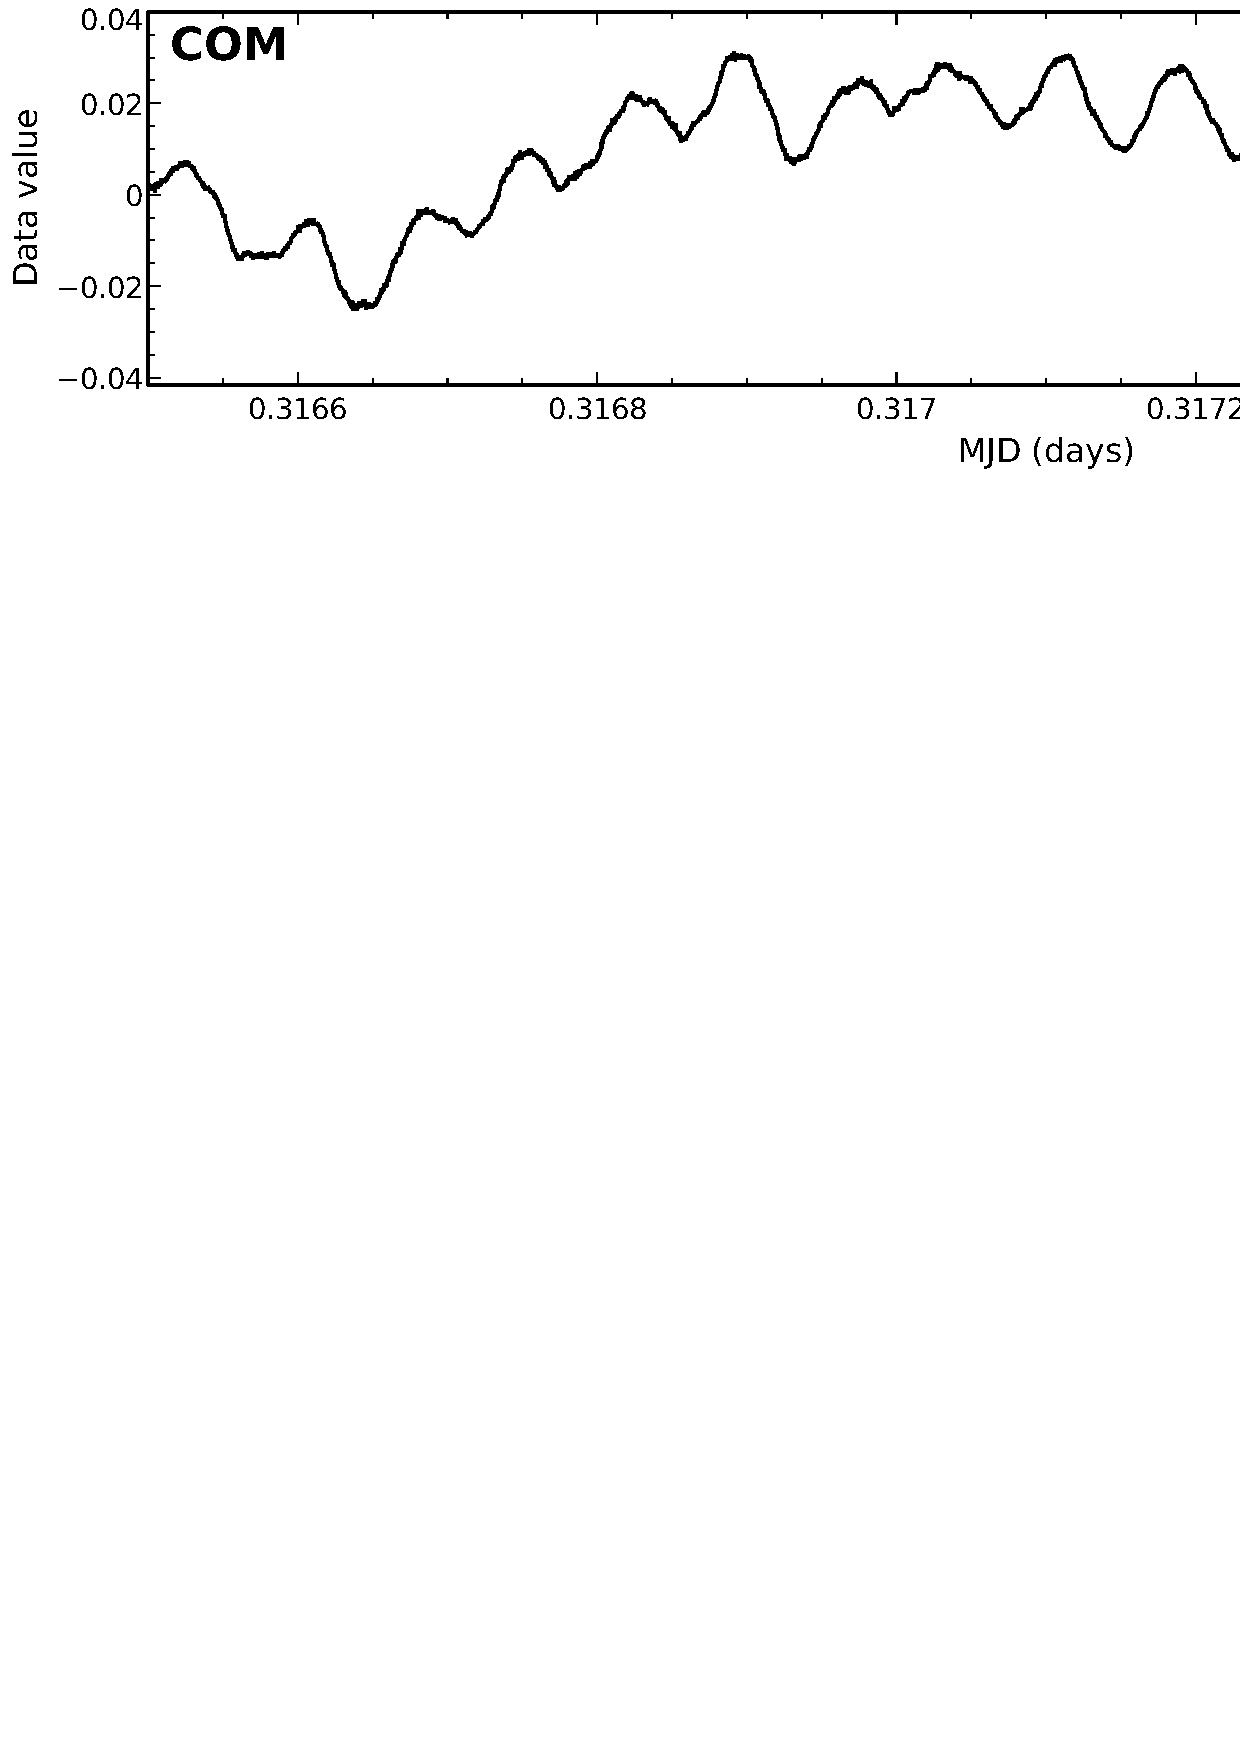
\includegraphics[width=\linewidth]{sc21_com} \\
  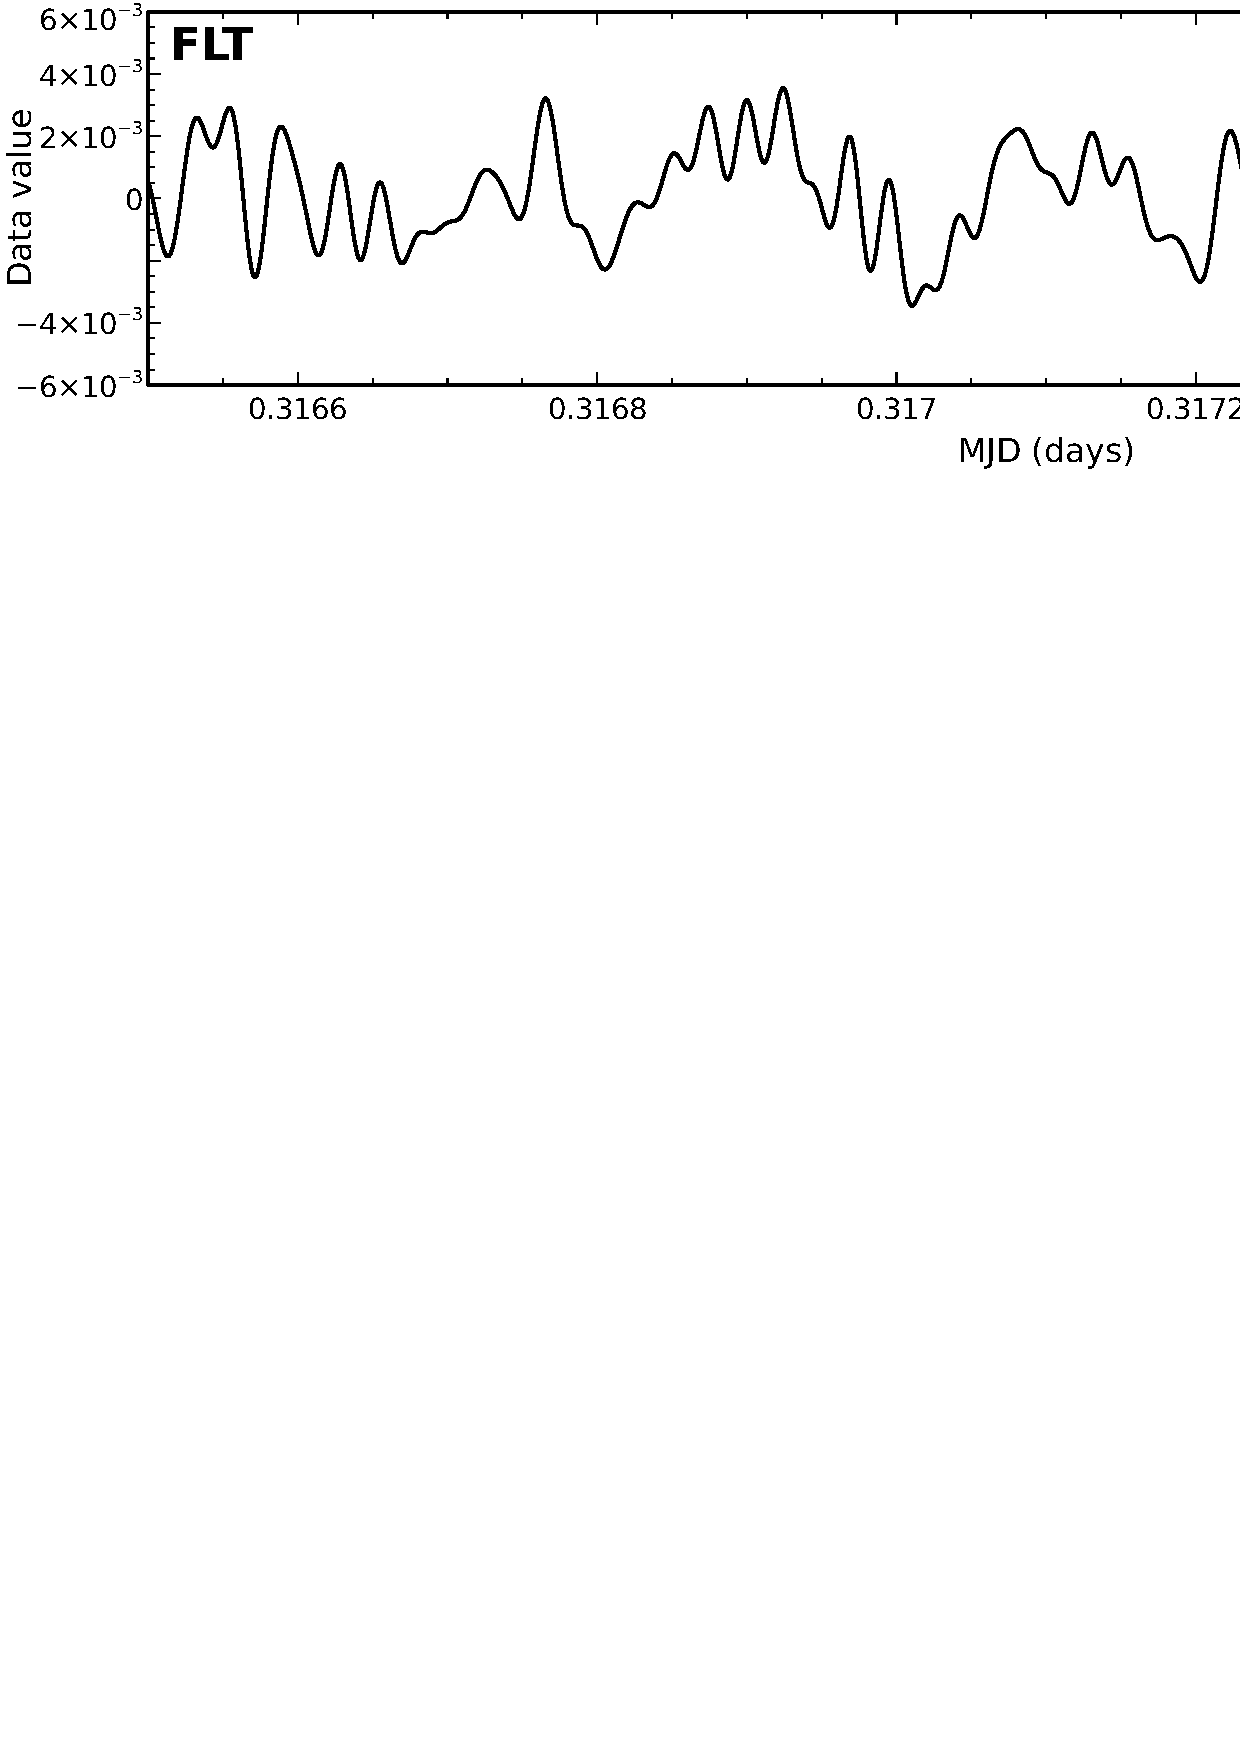
\includegraphics[width=\linewidth]{sc21_flt} \\
  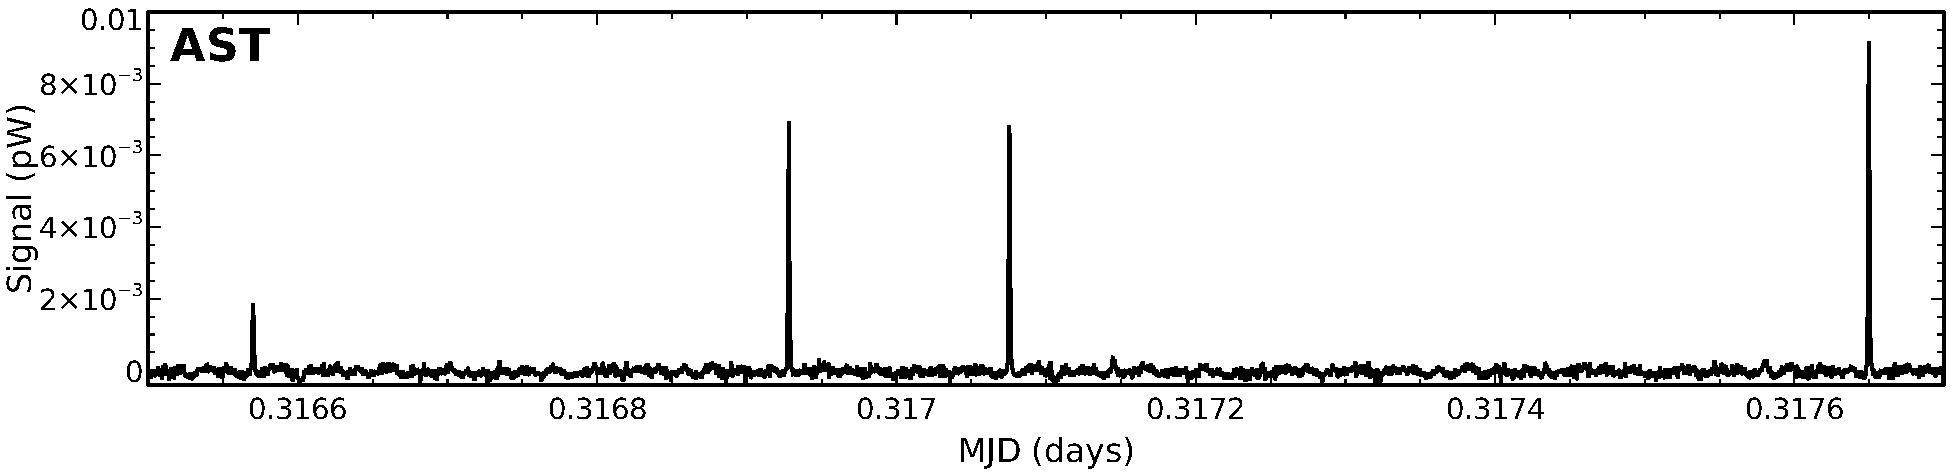
\includegraphics[width=\linewidth]{sc21_ast} \\
  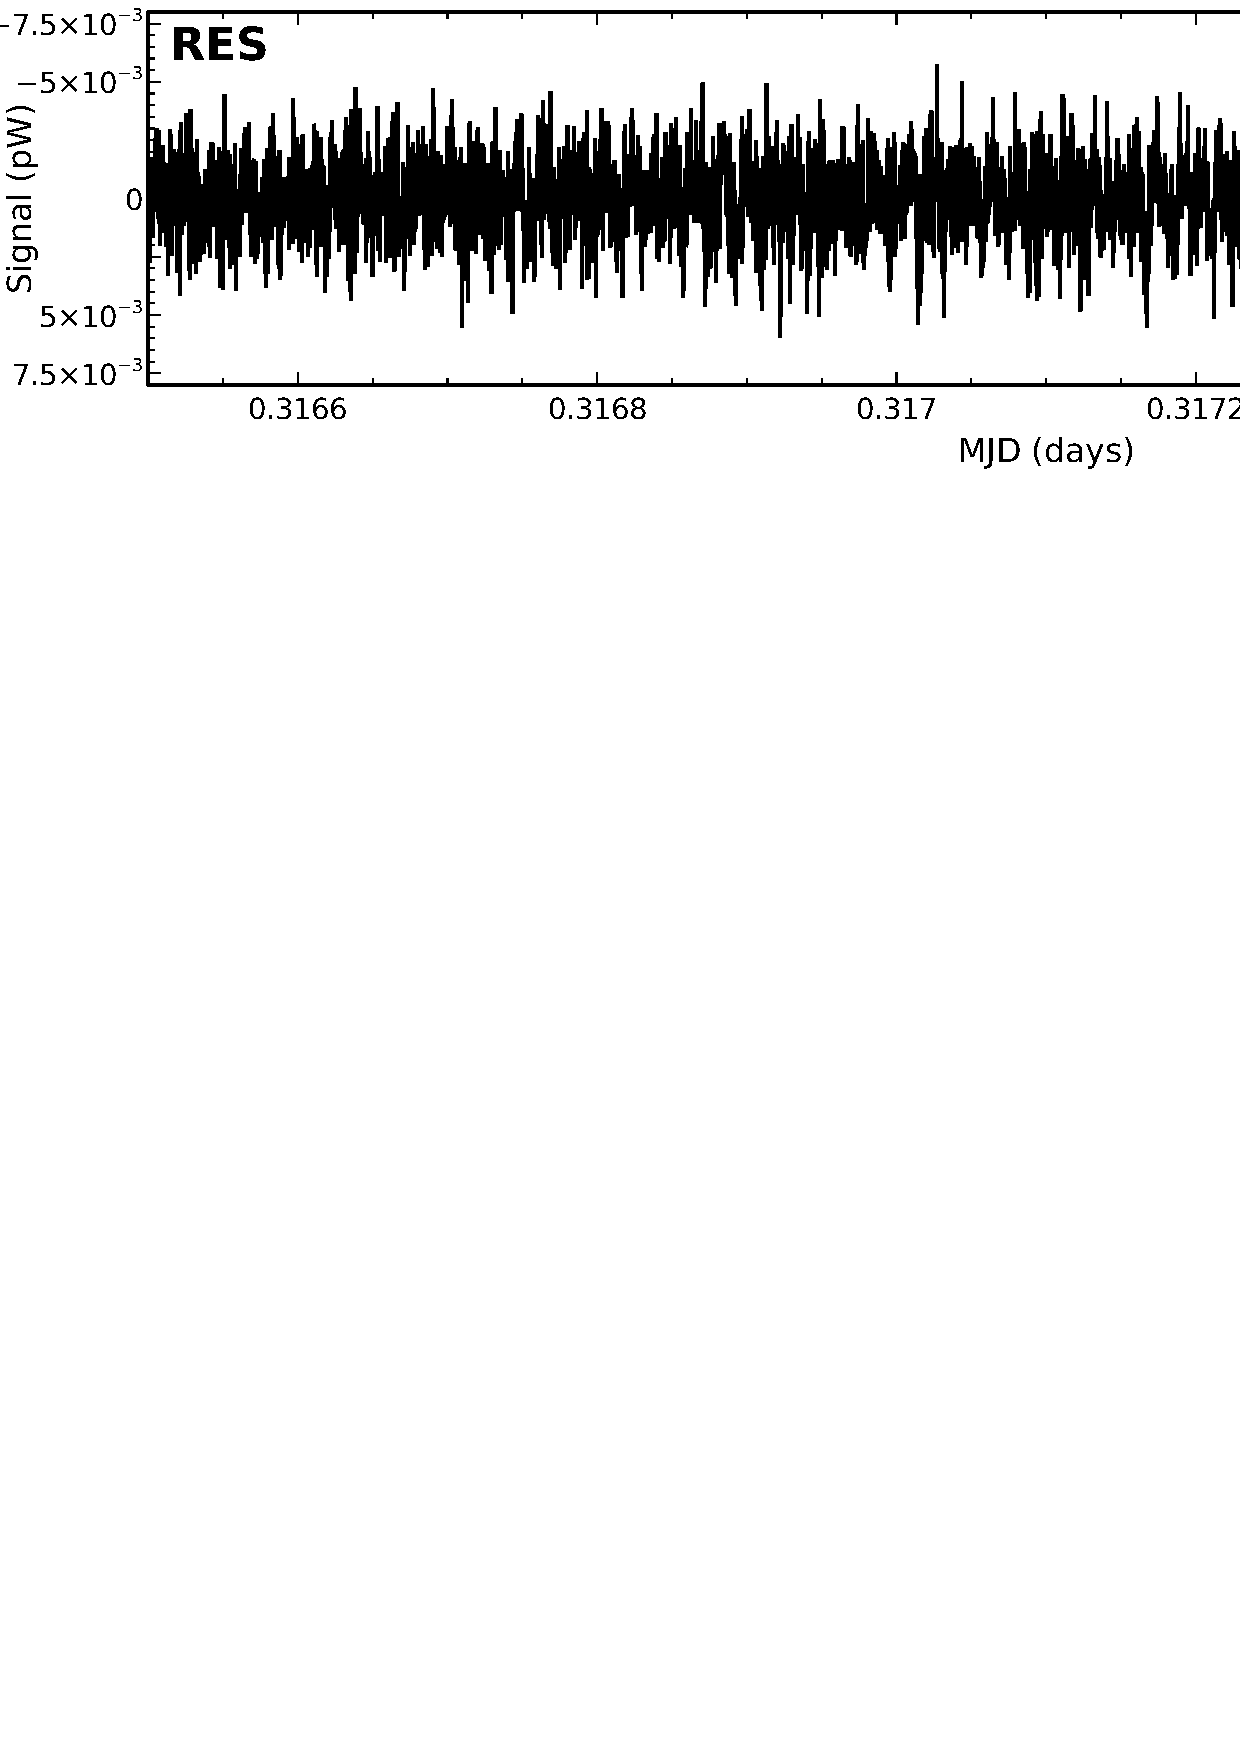
\includegraphics[width=\linewidth]{sc21_res} \\
\end{center}
\caption[Iterative models in the time domain]{\small Time-domain
components of the iterative models. These show the solution for the
same single bolometer for part of an observation of CRL~2688. From top
to bottom: the \model{COM} model containing signal common to all
bolometers, the \model{FLT} model containing residual low-frequency
noise missed by \model{COM}, the \model{AST} model with the signal
showing as a positive spike when this bolometer passes over the
source, and the \model{RES} model looking (as expected) like white
noise.}
\label{fig:itercomp}
\end{figure}


\section{\xlabel{export}Exporting individual models}
\label{sec:export}

By default, the final values of these fitted models are \emph{not}
written out. However, this can be changed by setting
\texttt{exportndf} in the configuration file to the list of models
that you wish to view.
%\vspace{0cm}

\begin{terminalv}
exportndf = (com,gai,ast,flt,res,noi,qua)
\end{terminalv}

In addition to the models listed in \cref{Section}{sec:models}{The
individual models}, you request \model{RES} in order to export the
residual model. \model{RES} is the residual signal remaining after
the other models have been removed. By contrast, the \model{NOI}
model is the noise in \model{RES}, as determined by running
\model{RES} through \calcnoise\ (see
\cref{Section}{sec:calcnoise}{Checking the array performance}). If
\model{NOI} is exported, it can be viewed as the VARIANCE component
of the \model{RES} model; thus, export of \model{RES} is implied if
\model{NOI} is specified.


The \texttt{exportndf} parameter will write out the requested models
as NDF files with names based on the first input file that went into
the maps for each sub-array. This is first suffixed by \texttt{con},
indicating that several data files may have been concatenated
together. The three-letter code for each model is then appended to the
filename (such as \file{s8a20120720\_00030\_0003\_con\_com.sdf},
\file{s8a20120720\_00030\_0003\_con\_flt.sdf},
\file{s8a20120720\_00030\_0003\_con\_res.sdf})\footnote{The filename
shows the third sub-scan of Observation 30 since this is the first science
file that is encountered (see \cref{Chapter}{sec:raw}{Handling Raw
SCUBA-2 Data}).~} The variance and quality for the data are stored as
the VARIANCE and QUALITY components within the residual file NDF.

\begin{tip}
  You can examine any of these model components as you would the final
  map.
\end{tip}

Examples of the time traces for a single bolometer from these output
models is shown in \cref{Figure}{fig:itercomp}{time-domain
components}. These traces cover a subset of an observation of the
secondary calibrator CRL~2688. You can clearly see the dominance of the
\model{COM} model which is removed first. The \model{FLT} model
stores the data removed by the high-pass filter. In the \model{AST}
model, CRL~2688 is clearly seen as positive spikes which appear when
the bolometer passes over the source. Finally, the residual signal
stored in \model{RES} is flat, indicating that most of the signal has
been successfully accounted for by the other model components.


\section{\xlabel{config}Specialised configuration files}
\label{sec:config}
The default configuration file \file{dimmconfig.lis} is intended to
provide a reasonably good map for all types of observations. However,
compromises have been made to reach that balance.

Whilst \file{dimmconfig.lis} is always a good recipe to start with
you will want to follow this up with a specialised recipe that will suit
your observation. A few specialised configuration files are supplied with
\smurf\ and can be found in \file{\$STARLINK\_DIR/share/smurf/}.

The specialised files are all based on \file{dimmconfig.lis}. This
is illustrated by \cref{Figure}{fig:configtree}{figure below} where
the parameters in \file{dimmconfig\_bright\_compact.lis} override
any identical ones in the hidden file \file{dimmconfig\_bright.lis} which in turn
override the values in \file{dimmconfig.lis}. The hierarchical
structure means the parameters at the top of the tree (or first
encountered) override any other instance of them.

\starfig{sc21_dimmcongitree}{[t]}{width=\linewidth}{fig:configtree}{
  Hierarchy of the configuration files}{
  Hierarchy of the configuration files.
}

Below is a description of each of the specialised configuration files.
The tables following each description list the parameters set for each
recipe. A verbatim copy of these files can be found in
\cref{Appendix}{app:special}{Specialised configuration files}.

\subsection{dimmconfig\_blank\_field.lis}

This configuration is tuned for blank field surveys for which the goal
is to detect extremely low signal-to-noise point sources.

Iteratively applying a high-pass filter (\model{FLT}) can result in
convergence problems when there is little or no signal in the
map. Instead, a single, harsher high-pass filter is applied as a
pre-processing step (corresponding to 200-arcsec scales at both
450\,$\mu$m and 850\,$\mu$m). There are also more conservative cuts to
remove noisy/problematic bolometers. Only 4 (positive) iterations are
requested as there is no signal to confuse to models.

The option \texttt{com.perarray}~=~1 requires the \model{COM} model to
be fit to each sub-array independently. This improves the overall fit
but with the loss of any structure on scales larger than a single
sub-array---not an issue for blank fields.

\cref{Figure}{fig:bfcompare}{The images below} shows the sharp
contrast in the output map between reducing data with the default
configuration file and using \file{dimmconfig\_blank\_field.lis}.

Blank-field maps commonly have a matched filter applied to aid source
detection (see \cref{Section}{sec:mf}{Point-source detection}),
however this is not applied by the map-maker.

\begin{figure}[t!]
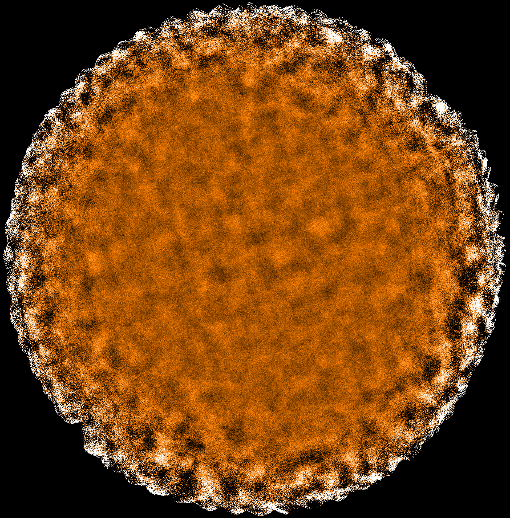
\includegraphics[width=0.47\linewidth]{sc21_cosmo1-def}
\hspace{3mm}
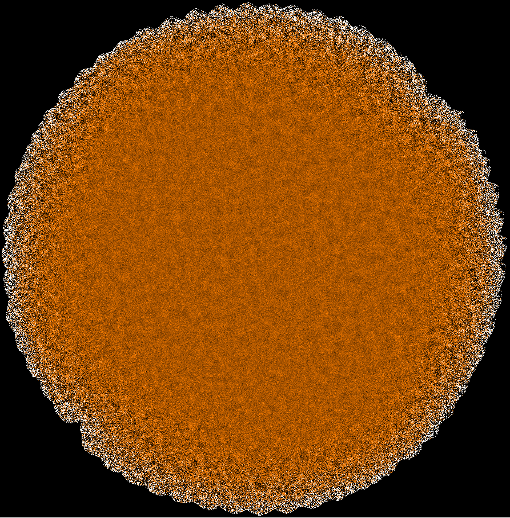
\includegraphics[width=0.47\linewidth]{sc21_cosmo1-bf}
\caption[Example map reduced with \file{dimmconfig\_blank\_field.lis}]{
    Maps of a deep cosmology field reduced with \textbf{(left)}
    \file{dimmconfig.lis} and \textbf{(right)}
    \file{dimmconfig\_blank\_field.lis} \label{fig:bfcompare}}.
\end{figure}



% The tildes around the equal sign are to ensure HTML table field is
% not wrapped after the parameter name.
\renewcommand*\arraystretch{0.95}
\begin{table}[h!]
\centering
\begin{tabular}{|p{6.5cm}p{7.0cm}|}
\hline
\multicolumn{2}{|l|}{\file{dimmconfig\_blank\_field.lis}}\\
\hline
\param{numiter~=~4}&\param{flt\_edge\_largescale~=~200}\\
\param{spikethresh~=~10}&\param{model order~=~(com,ext,ast,noi)}\\
\param{com.perarray~=~1}&\\
\hline
\end{tabular}
\end{table}




\subsection{dimmconfig\_bright\_compact.lis}

This configuration is aimed at reducing maps of bright, compact
sources that are isolated at the centre of the map (i.e. calibrators). It references
\file{dimmconfig\_bright.lis}, and thus the parameters from both `bright'
recipes override the default values in \file{dimmconfig.lis}.

The addition of \param{ast.zero\_circle} and
\param{ast.zero\_notlast} parameters are used to constrain the map to
zero beyond a radius of 1\,arcmin for all but the final iteration.
This strategy helps with map convergence significantly, and can
provide good maps of bright sources, even in cases where scan patterns
failed to complete in full.

\param{com.perarray} is set to 1 indicating that a \model{COM} model
should be fit separately for each sub-array. This is not advised for
extended sources as signal on scales larger than a single sub-array is
lost, but is fine for a compact central source. Likewise, the filtering
is tighter. The S/N threshold for DC steps (\param{dcthresh}) is relaxed from
25 in the default file to 100 to avoid problems associated with bright sources.

% The tildes around the equal sign are to ensure HTML table field is
% not wrapped after the parameter name.
\latex{\renewcommand*\arraystretch{0.95}}
\begin{table}[h!]
\centering
\begin{tabular}{|p{6.5cm}p{7.0cm}|}
\hline
\multicolumn{2}{|l|}{\file{dimmconfig\_bright\_compact.lis}}\\
\hline
\param{numiter = -40}&\param{flt.filt\_edge\_largescale~=~200}\\
\param{com.perarray~=~1}&\param{flt.zero\_circle~=~(0.016666)}\\
 \param{ast.zero\_circle~=~(0.0166666666)}&\\
\hline
\multicolumn{2}{|l|}{\param{dimmconfig\_bright.lis}}\\
\hline
\param{noisecliphigh~=~10.0} & \param{dcthresh~=~100}\\
\param{com.corr\_tol~=~7}& \param{com.gain\_tol~=~7}\\
\param{com.gain\_abstol~=~5}& \\
\hline
\end{tabular}
\end{table}


\subsection{dimmconfig\_bright\_extended.lis}

\begin{figure}[t!]
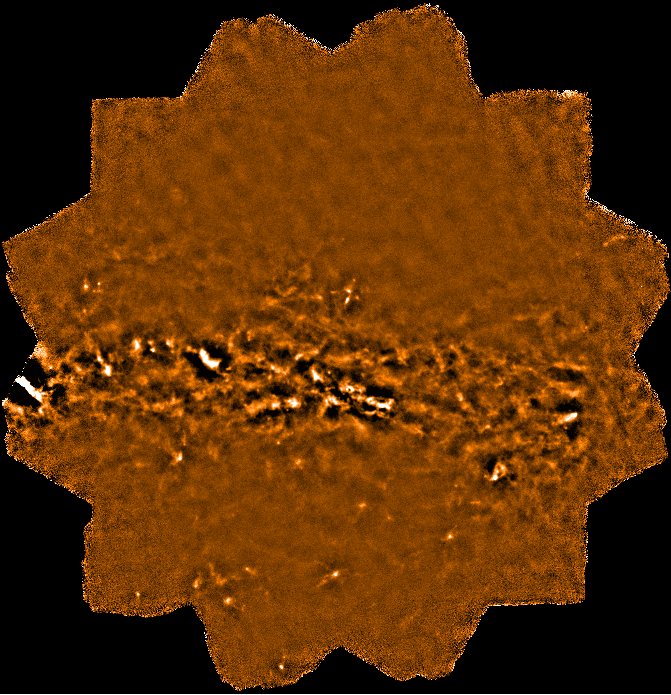
\includegraphics[width=0.47\linewidth]{sc21_gal_def}
\hspace{3mm}
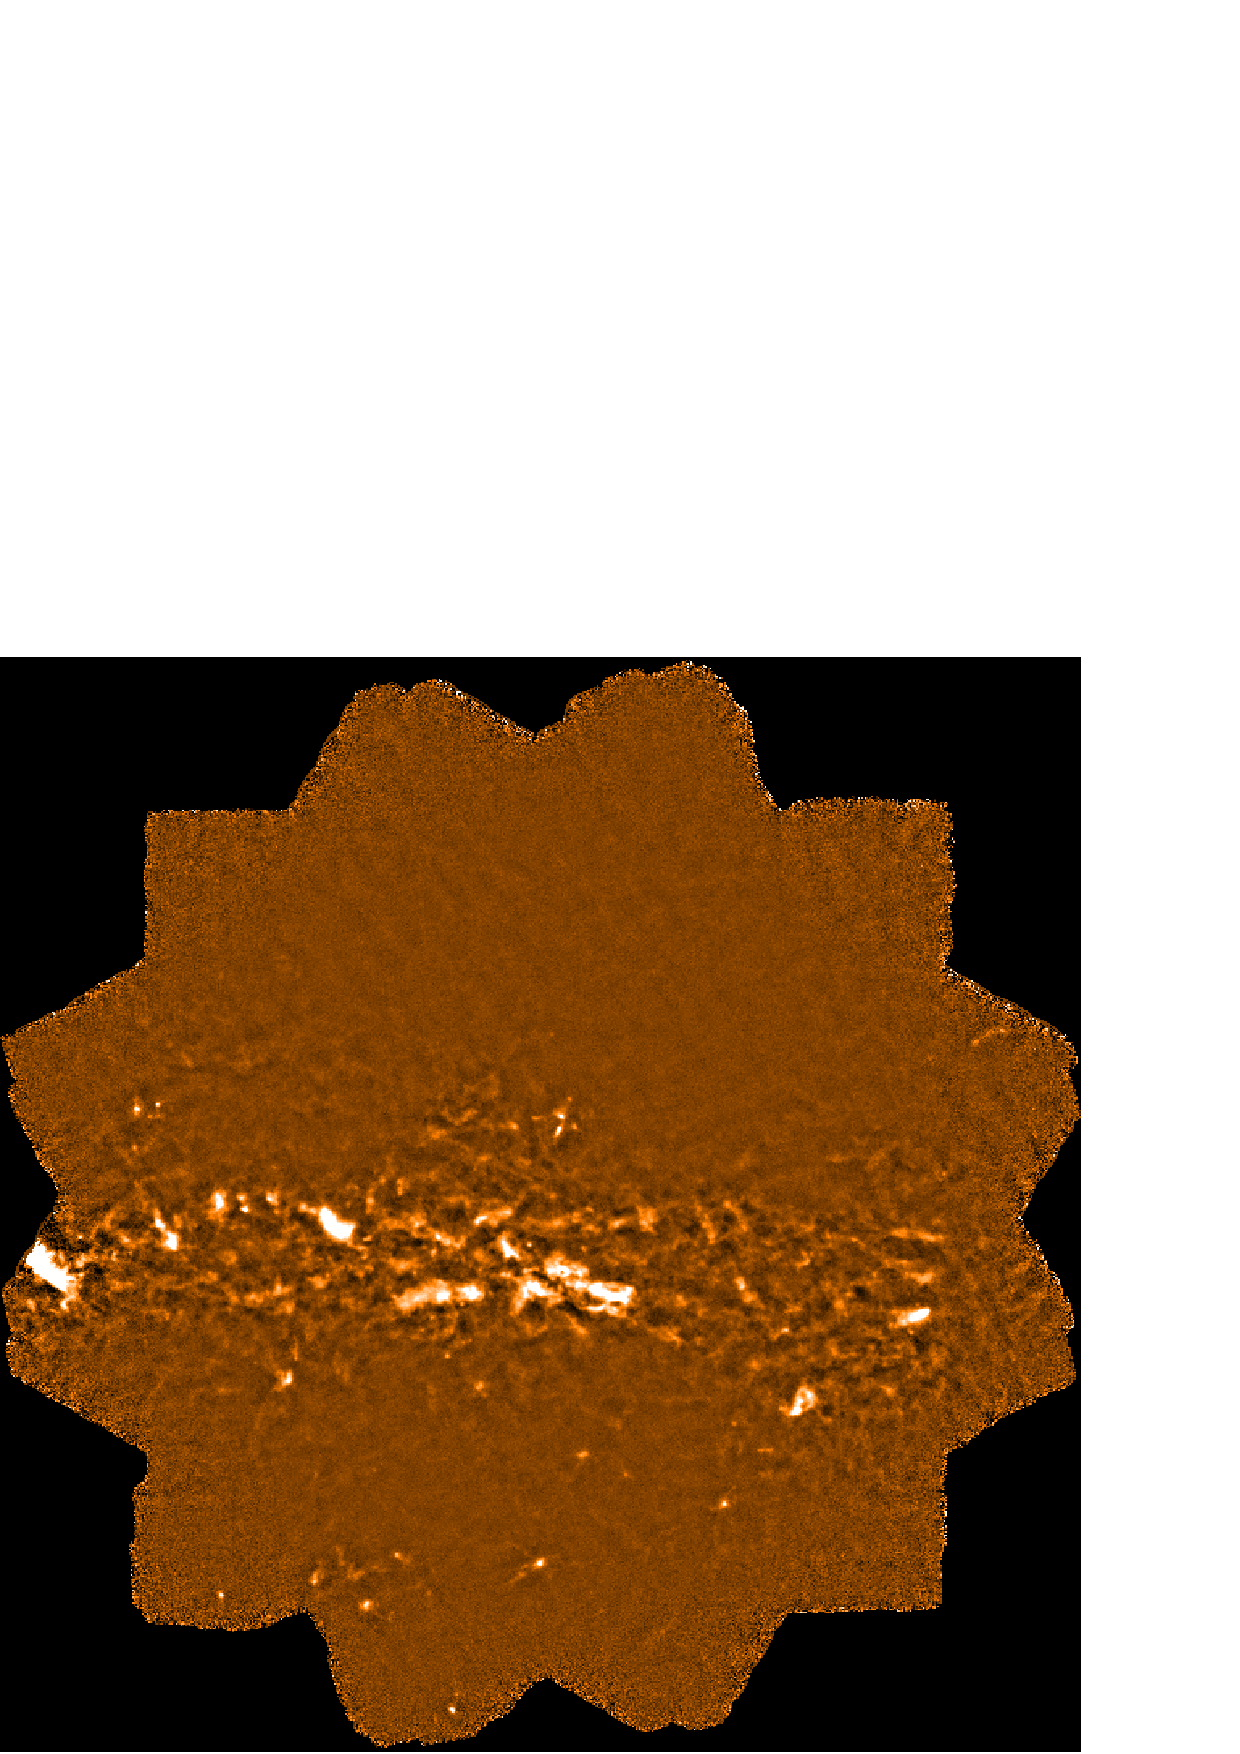
\includegraphics[width=0.47\linewidth]{sc21_gal_brex}
\caption[Example map reduced with
  \file{dimmconfig\_bright\_extended.lis}]
 {A region towards the Galactic Centre reduced with \textbf{(left)}
   \file{dimmconfig.lis} and \textbf{(right)}
   \file{dimmconfig\_bright\_extended.lis}.\label{fig:becompare}}
\end{figure}

This configuration is for reducing maps that do not fall into the
other two categories. The emission is usually extended to some degree
and contains some bright regions. Here \param{ast.zero\_snr} is used
to constrain the \model{AST} model to zero wherever the S/N is lower
than 5$\sigma$.  Everywhere the signal is below this threshold, the
map is set to zero for all but the final iteration. \param{numiter}
has been raised to \texttt{-40}, as more iterations are required to
maximise the sensitivity to large dynamic signal ranges in the map.

Recovering both faint extended structure and bright sources in the
same field poses an extra challenge. Strategies for this are explored
in \cref{Chapter}{sec:tweak}{Tailoring Your Reduction}.

\cref{Figure}{fig:becompare}{The images below} shows a comparison
between maps reduced with the default configuration file and using
\file{dimmconfig\_bright\_extended.lis}; the most noticeable
difference is the improvement in the bowling around strong sources.

\latex{\renewcommand*\arraystretch{1}}
\begin{table}[h!]
\centering
\begin{tabular}{|p{6.5cm}p{6.5cm}|}
\hline
\multicolumn{2}{|l|}{\file{dimmconfig\_bright\_extended.lis}}\\
\hline
\param{numiter~=~-40}&\param{flt.filt\_edge\_largescale~=~480}\\
\param{ast.zero\_snr~=~3}&\param{ast.zero\_snrlo~=~2}\\
\param{ast.skip~=~5}&\param{flt.zero\_snr~=~5}\\
\param{flt.zero\_snrlo~=~3}& \\
\hline
\end{tabular}
\end{table}


\section{\xlabel{problem}Solving configuration-file problems}
\label{sec:problem}

Two trouble-shooting configuration files are available to supplement your
configuration file.
\begin{itemize}[noitemsep]
\item \file{dimmconfig\_fix\_convergence} to help your map converge.
\item \file{dimmconfig\_fix\_blobs} to remove large blooms or blobs of spurious
emission in your map.
\end{itemize}
By default these recipes do not point to any existing configuration file. To use
these recipes in addition to  \file{dimmconfig\_bright\_extended.lis} you should
create a parameter file containing the following lines.

\begin{terminalv}
^/star/share/smurf/dimmconfig_bright_extended.lis
^/star/share/smurf/dimmconfig_fix_blobs.lis
\end{terminalv}

This reads a complete set of configuration parameter from the
\file{dimmconfig\_bright\_extended.lis} file, and then assigns new values for just
those parameters defined in \file{dimmconfig\_fix\_blobs.lis}. These values override
the values specified in \file{dimmconfig\_bright\_extended.lis}.

The parameters in these recipes are discussed further
\cref{Chapter}{sec:tweak}{Tailoring Your Reduction}.



\chapter{\xlabel{maps}Reducing Your Data}
\label{sec:maps}

This chapter describes how to run the map-maker and what to look out
for during processing. We also discuss reducing your data using the
\oracdr\ science pipeline and why you might want to chose this option.

As discussed in \cref{Chapter}{sec:dimm}{The
Dynamic Iterative Map-Maker}, all of the settings for the map-maker
are stored in configuration files. In this chapter we use
the default configuration file, \file{dimmconfig.lis} to reduce CRL~2688,
one of SCUBA-2's secondary calibrators. For an
overview of the specialised configuration files available see
\cref{Section}{sec:config}{this section}.

\section{\xlabel{running_dimm}Running the iterative map-maker}
\label{sec:running}

When running the map-maker, you can call any of the provided
configuration files directly from the Starlink path (e.g.
\file{\^{}\$STARLINK\_DIR/share/smurf/dimmconfig.lis}). Alternatively,
a local copy can be made and edited. Advice on which parameters to
edit can be found in \cref{Section}{sec:tweak}{Tweaking the
configuration file}.

\begin{tip}
  An up-caret (\,\texttt{\^{}}\,) is required any time you are reading
  in a group text file in \starlink. For the map-maker this includes
  the configuration file (a group of parameters) and a list of your
  input files (e.g. \texttt{in=\^{}\,myrawfiles.txt}).
\end{tip}


The default pixel sizes are:
\begin{itemize}
\item 2\,arcsec at 450$\mu$m
\item 4\,arcsec at 850$\mu$m
\end{itemize}

These can be changed by adding the \texttt{pixsize=}$x$ to the
command string\footnote{The default sizes are defined as one quarter
of the Airy disk rounded up to the nearest half arcsecond.}, where $x$
is your desired pixel size in arcsecs. We advise that you do not
increase the pixel size at this stage as it will compromise model
fitting---instead regrid your map as a post-processing step.

% Other ADAM parameter available with \makemap\ include ref, maxmem
% and msg\_filter. Some of these appear in the example below but see
% \cref{Appendix}{app:adam}{MAKEMAP ADAM Parameters} for
% descriptions. A complete list of all ADAM parameters can be found in
% \smurfsun.

\begin{tip}
  Map-maker not finding your raw files from a path? Check you have
  double quotes around your `in' option and are not using
  \texttt{*sdf}---use either \texttt{*.sdf} or just \texttt{*}.
\end{tip}



\begin{terminalv}
% makemap in="/jcmtdata/raw/scuba2/s8*/20120720/00030/*.sdf" out=850_crl2688 \
  config=^$STARLINK_DIR/share/smurf/dimmconfig.lis

Out of 32 input files, 4 were darks, 8 were fast flats and 20 were science
Processing data from instrument 'SCUBA-2' for object 'CRL2688' from the
following observation  :
  20120720 #30 scan  /shutter

MAKEMAP: Map-maker will use no more than 68401 MiB of memory

Projection parameters used:
CRPIX1 = 0
CRPIX2 = 0
CRVAL1 = 315.578333333333 ( RA = 21:02:18.800 )
CRVAL2 = 36.6938055555556 ( Dec = 36:41:37.70 )
CDELT1 = -0.00111111111111111 ( -4 arcsec )
CDELT2 = 0.00111111111111111 ( 4 arcsec )
CROTA2 = 0

Output map pixel bounds: ( -132:122, -126:129 )

Output map WCS bounds:
Right ascension: 21:01:38.318 -> 21:03:03.280
Declination: 36:33:07.19 -> 36:50:11.70

smf_iteratemap: will down-sample data to match angular scale of 4 arcsec
smf_iteratemap: Iterate to convergence (max 5)
smf_iteratemap: stop when change in chi^2 < 0.001
smf_iteratemap: provided data are in 1 continuous chunks, the largest of which
has 5957 samples (153.729 s)
smf_iteratemap: map-making requires 1376 MiB (map=3 MiB model calc=1372 MiB)
smf_iteratemap: Continuous chunk 1 / 1 =========
smf_calc_smoothedwvm: 0.977444 s to calculate unsmoothed WVM tau values
smf_iteratemap: Iteration 1 / 5 ---------------
--- Size of the entire data array ------------------------------------------
bolos  : 5120
tslices: bnd:0(0.0 min), map:5957(2.6 min), tot:5957(2.6 min)
Total samples: 30499840
--- Quality flagging statistics --------------------------------------------
 BADDA:   10972794 (35.98%),        1842 bolos
BADBOL:   11818688 (38.75%),        1984 bolos
DCJUMP:      38809 ( 0.13%),
  STAT:      71680 ( 0.24%),          14 tslices
 NOISE:     810152 ( 2.66%),         136 bolos
Total samples available for map:   18634826, 61.10% of max (3128.22 bolos)
smf_iteratemap: Calculate time-stream model components
smf_iteratemap: Rebin residual to estimate MAP
smf_iteratemap: Calculate ast
--- Quality flagging statistics --------------------------------------------
 BADDA:   10972794 (35.98%),        1842 bolos  ,change          0 (+0.00%)
BADBOL:   11925914 (39.10%),        2002 bolos  ,change     107226 (+0.91%)
DCJUMP:      38809 ( 0.13%),                    ,change          0 (+0.00%)
  STAT:      71680 ( 0.24%),          14 tslices,change          0 (+0.00%)
   COM:     323165 ( 1.06%),                    ,change     323165 (+0.00%)
 NOISE:     810152 ( 2.66%),         136 bolos  ,change          0 (+0.00%)
Total samples available for map:   18312771, 60.04% of max (3074.16 bolos)
     Change from last report:    -322055, -1.73% of previous
smf_iteratemap: Will calculate chi^2 next iteration
smf_iteratemap: *** NORMALIZED MAP CHANGE: 0.874979 (mean) 73.7106 (max)
smf_iteratemap: Iteration 2 / 5 ---------------
smf_iteratemap: Calculate time-stream model components
smf_iteratemap: Rebin residual to estimate MAP
smf_iteratemap: Calculate ast
--- Quality flagging statistics --------------------------------------------
 BADDA:   10972794 (35.98%),        1842 bolos  ,change          0 (+0.00%)
BADBOL:   11949742 (39.18%),        2006 bolos  ,change      23828 (+0.20%)
 SPIKE:         34 ( 0.00%),                    ,change         34 (+0.00%)
DCJUMP:      38809 ( 0.13%),                    ,change          0 (+0.00%)
  STAT:      71680 ( 0.24%),          14 tslices,change          0 (+0.00%)
   COM:     357816 ( 1.17%),                    ,change      34651 (+10.72%)
 NOISE:     810152 ( 2.66%),         136 bolos  ,change          0 (+0.00%)
Total samples available for map:   18278374, 59.93% of max (3068.39 bolos)
     Change from last report:     -34397, -0.19% of previous
smf_iteratemap: *** CHISQUARED = 0.983228126551834
smf_iteratemap: *** NORMALIZED MAP CHANGE: 1.29181 (mean) 15.0552 (max)
smf_iteratemap: Iteration 3 / 5 ---------------
.....
.....
.....
smf_iteratemap: Iteration 5 / 5 ---------------
smf_iteratemap: Calculate time-stream model components
smf_iteratemap: Rebin residual to estimate MAP
smf_iteratemap: Calculate ast
--- Quality flagging statistics --------------------------------------------
 BADDA:   10972794 (35.98%),        1842 bolos  ,change          0 (+0.00%)
BADBOL:   11949742 (39.18%),        2006 bolos  ,change          0 (+0.00%)
 SPIKE:         34 ( 0.00%),                    ,change          0 (+0.00%)
DCJUMP:      38809 ( 0.13%),                    ,change          0 (+0.00%)
  STAT:      71680 ( 0.24%),          14 tslices,change          0 (+0.00%)
   COM:     362902 ( 1.19%),                    ,change          0 (+0.00%)
 NOISE:     810152 ( 2.66%),         136 bolos  ,change          0 (+0.00%)
Total samples available for map:   18273302, 59.91% of max (3067.53 bolos)
     Change from last report:          0, +0.00% of previous
smf_iteratemap: *** CHISQUARED = 0.952708604771402
smf_iteratemap: *** change: -0.000109049487216351
smf_iteratemap: *** NORMALIZED MAP CHANGE: 0.107427 (mean) 2.96138 (max)
smf_iteratemap: ****** Completed in 5 iterations
smf_iteratemap: ****** Solution CONVERGED
Total samples available from all chunks: 18273302 (3067.53 bolos)
%%%%\end{}
\end{terminalv}



\section{\xlabel{look_for}What to look out for}
\flushbottom

Once the map-maker has completed you can open your output map using
\gaia\ (see \cref{Figure}{fig:itermap}{this example}). The excerpt in
\cref{Section}{sec:running}{Running the iterative map-maker} shows the
output written to the terminal as you run the map-maker. There are a
number of clues in this output that indicate the status of the
reduction.

\starfig{sc21_crl2688}{[t!]}{width=0.7\linewidth}{fig:itermap}{
  CRL~2688 produced with \makemap}{
  Map of CRL~2688 produced with the \smurf\ task \makemap\ using the
  iterative algorithm with default parameters.
}


\begin{description}
\item[The number of input files] The first to note is the number of
  input files; it is worth checking this matches your expected
  number. Also summarised are the source name, UT date and scan
  number.

\item[Map dimension] Next the basic dimensions of the data being
  processed are listed near the start of the first iteration. The
  example above has 4\,arcsec pixels---the default at 850$\mu$m.


\item[Chunking] The map-maker then determines if the raw data should
  be split and processed in more than one chunk. In this map the data
  are reduced in one continuous piece: \param{Continuous chunk 1 /
    1}. Chunking is where the map-maker processes sub-sections of the
  time-series data independently and should be avoided if
  possible---see the text box below.
\end{description}


\subsubsection*{Quality statistics}

At the beginning of the reduction, the main purpose of QUALITY
flagging is to indicate how many bolometers are being used. In the
example above you can see that from a total of 5120 bolometers, 1842
were turned off during data acquisition (\texttt{BADDA}). In addition,
136 bolometers exceeded the acceptable noise threshold
(\texttt{NOISE}), while tiny fractions of the data were flagged
because the telescope was moving too slowly (\texttt{STAT}) or the
sample are adjacent to a step that was removed (\texttt{DCJUMP}).

The total number of bad bolometers (\texttt{BADBOL}) is 1984.
Accounting for these, and the small numbers of additionally flagged
samples, 3128.22 effective bolometers are available after initial
cleaning\footnote{The fractional number is due to time-slices being
removed during cleaning. The number of bolometers is then
reconstructed from the number of remaining time-slices.}.


\begin{sltextbox}{Data Chunking}
  \label{box:chunk}
  Chunking occurs when there is insufficient computer memory available
  for the map-maker or when there is a gap in the time-series data
  (e.g.  from a missing sub-scan). In these cases, the map-maker
  divides up the time-series data and reduces each sub-portion
  independently, before re-combining all the outputs at a later
  stage. Ideally you want your data reduced in a single chunk, however
  this can be unfeasible for large maps.

  The more data the map-maker processes at once, the better chance it
  has of determining the difference between sky signal and background
  noise.

  In \textsc{daisy} mode chunking is less of a concern as the entire
  map area is covered many times in the space of a single observation.

  For \textsc{pong} maps chunking is a bigger concern, with the
  maximum number of chunks that can be tolerated dependent on the
  number of map rotations. For example, a 40-minute \textsc{pong} map
  with eight rotations may get divided into three or four
  chunks. Although not ideal, this will mean that each point is still
  covered by two or three passes. Fewer passes than this however and
  the map-maker become less effective.
\end{sltextbox}

After each subsequent iteration a new `Quality' report is produced,
indicating how the flags have changed. An important flag that appears
in the `Quality' report following the first iteration is \model{COM}:
the DIMM rejects bolometers (or portions of their time series) if they
differ significantly from the common-mode (average) of the remaining
bolometers.

You may note that compared with the initial report, the total number
of samples with good `Quality' (\texttt{Total samples available for
  map}) has dropped from 18634826 to 18273302 (about a 2 per cent
decrease) as additional samples were flagged in each iteration.

Be aware that some large reductions may take many iterations to reach
convergence and you may find significantly fewer bolometers remaining
resulting in higher noise than expected.

\subsubsection*{Convergence}

The convergence criteria \param{maptol} is updated for each
iteration. The convergence can be checked from the line reporting\\*
\hspace*{0.5cm} \texttt{smf\_iteratemap: *** NORMALIZED MAP CHANGE:
  0.10559 (mean) 2.81081 (max)}

The number to look out for is the mean value. This will have to drop
below your required \param{maptol} for convergence to be achieved.

The default configuration file used in this example executes a maximum
of five iterations, but stops sooner if the change in \param{maptol}
drops below 0.05 (i.e. \param{numiter~=$-$5}). In this example it
stops after five iterations.



\begin{tip}
  You can interrupt the processing at any stage with a single
  \texttt{Ctrl-C}. The map-maker will complete the iteration then
  write out a final science map. Entering \texttt{Ctrl-C} twice will
  kill the process immediately.\widowpenalty=100000
\end{tip}

\section{\xlabel{sciencepl}Using the science pipeline}

You can also reduce your data using the \oracdr\ science pipeline on a
local computer. There are advantages to running the map-maker using
the pipeline. You can feed the pipeline observations of multiple
sources rather than feed in a single source at a time. The pipeline
will recognise the different sources and make a separate map for each,
whereas the map-maker would make a single large map that would include
all your sources (no matter how widely spaced!).

Another useful feature is that the pipeline will generate a log files
to record various useful quantities. The standard log files from
reducing science data are:

\begin{itemize}
\item \file{log.noise}---noise in the map for each observation and the co-add
(calculated from the median of the error array), and
\item \file{log.nefd}---NEFD calculated for each observation and for
the co-added map(s).
\end{itemize}
The pipeline will produce calibrated maps; by default these are
calibrated using the standard FCFs, although you can specify your
own if you wish.

Running the science pipeline is very straightforward and can be as
simple as the example below. Here a list is made of all your raw data,
the pipeline is then initiated, finally the reduction is started with
instructions to loop through all data listed in the supplied file and
the filename in question is given.

\begin{terminalv}
% ls s8*.sdf > myfiles.lis
% oracdr_scuba2_850
% oracdr -loop file -files myfiles.lis
\end{terminalv}

\textbf{For a more in-depth discussion on running the pipeline and a
  discussion of the various outputs see \cref{Chapter}{sec:pipe}{The
    SCUBA-2 Pipeline} or \pipelinesun.}



\chapter{\xlabel{postprocess}Post-processing Reduction Steps}
\label{sec:postprocess}

\section{\xlabel{apply_fcf}Flux conversion factors}
\label{sec:cmult}

When your data comes out of the map-maker it is in units of picowatts
(pW). A flux conversion factor, or FCF, needs to be applied to scale
your data from units of pW to janskys (Jy). For more information on
calibrating SCUBA-2 data see Dempsey et al. (2013) \cite{dempsey12}.


Below are our default FCFs.
\vspace{0.5cm}
\renewcommand*\arraystretch{1.2}

\begin{table}[h!]
\centering
\begin{tabular}{|c|c|c|c|}
\hline
\multicolumn{2}{|c|}{\textbf{APERTURE}}  &
\multicolumn{2}{c|}{\textbf{PEAK}}      \\
\hline
\multicolumn{2}{|c|}{\fcfa\ (Jy/pW/arcsec$^2$) }  &
\multicolumn{2}{c|}{\fcfb\ (Jy/pW/beam)}      \\
\hline
\hspace{0.4cm} 450\,$\mu$m \hspace{0.3cm} & 850\,$\mu$m & \hspace{0.4cm} 450\,$\mu$m \hspace{0.3cm}& 850\,$\mu$m \\
\hline
4.71 $\pm$ 0.5& 2.34 $\pm$ 0.08& 491 $\pm$ 67& 537 $\pm$ 24 \\
\hline
\end{tabular}
\end{table}
\renewcommand*\arraystretch{1.0}
\vspace{0.5cm}

\begin{sltextbox}{IMPORTANT NOTES:}
  \begin{itemize}
  \item The standard FCF to be applied depends on the reduction date
    for your data. For data that have been \emph{reduced prior} to
    July 2012 you should see \cref{Appendix}{app:fcfs}{FCFs by
      reduction date} for alternative FCFs.

  \item Due to a glitch in the WVM, data reduced between 2012
    September 19, and 2013 January 18 must be re-reduced using a
    recent version of Starlink (Hikianalia or later), or should have
    an FCF derived from a calibrator reduced at the same time (and not
    our standard FCF) applied to it.
  \end{itemize}
\end{sltextbox}


\subsection{Aperture flux}

To get the flux density of extended sources with aperture photometry
you should apply the \fcfa.  You can then sum the emission in an
aperture. \fcfa\ was determined using a 60-arcsec diameter
aperture. If your aperture differs from this you should scale your
flux accordingly---the scaling factor can be read off the curve of
growth (see \cref{Appendix}{app:cog}{this appendix}). This graph gives
the ratio of aperture flux to total flux for a range of aperture
diameters.

\fcfa\ is determined using 1-arcsec pixels. For different pixel sizes
you will also need to multiply by the pixelsize squared.

\subsection{Peak flux}

If you want to read off the peak flux from your map, you should apply
the \fcfb\ (also known as the peak FCF).  When you open your map in
\gaia\ the value of the brightest pixel will be the peak flux of your
source. (If your source is point-like, the peak value in the map is
the total flux density). Applying \fcfb\ will result in a map with
units of Jy/beam. For point-like or compact sources smaller than the
beam (with a Gaussian profile), this peak value will be the flux
density of your source.

\subsection{Determining your own FCF}

Calibration observations are taken at various points throughout the
night and we recommend you compare the FCF calculated from your
nearest calibrator to the standard FCF. You can use this FCF to scale
the the standard value accordingly. You should chose the calibrator
nearest in time to your science observations, unless the weather has
changed significantly.

\begin{enumerate}
\item Reduce the calibrator with the map-maker using
  \file{dimmconfig\_bright\_compact.lis} as the configuration file.

\item Determine the FCF value by passing the output map to the
  \picard\ recipe
  \xref{\drrecipe{SCUBA2\_CHECK\_CAL}}{sun265}{SCUBA2_CHECK_CAL}.
\begin{terminalv}
% picard SCUBA2_CHECK_CAL 850calibrator.sdf
\end{terminalv}
This will produce a log file (\file{log.checkcal}) which records the
both \fcfb\ and \fcfa. Check that these values closely approximate the
standard FCF values given above.

\item Re-reduce the calibrator using the map-maker with the
  \emph{same} configuration file you used for your science
  observations.

\item Again determine the FCF using \drrecipe{SCUBA2\_CHECK\_CAL}.

\item Apply this FCF to your reduced science data using \cmult---see
  the next section. Remember to apply the pixel size squared factor if
  using \fcfa.
\end{enumerate}

\subsection{Applying the FCF}

You can apply the FCF using the \picard\ recipe
\xref{\drrecipe{CALIBRATE\_SCUBA2\_DATA}}{sun265}{CALIBRATE\_SCUBA2\_DATA}.
By default this will multiply your map by 1000$\times$\fcfb, obtained
from the start of \cref{Section}{sec:cmult}{Flux conversion
  factors}. This produces a calibrated map with units of mJy/beam.

You can supply a parameter file if you wish to use a different value
for the FCF or use \fcfa. The recipe will write out the calibrated
file with an \file{\_cal} suffix and will change the units in the map
header.

\begin{terminalv}
% picard CALIBRATE_SCUBA2_DATA  mapinpW.sdf
\end{terminalv}
Note that the recipe will also take account of the pixel size when
applying \fcfa.


\section{\xlabel{crop}Cropping your map}
\label{sec:crop}

The nature of the scan patterns results in SCUBA-2 maps significantly
larger than the requested size. The high noise towards the outer edges
is a consequence of the scanning pattern. Although this excess data
are down-weighted during reduction by the map-maker, you may wish to
remove it before either combining maps (see
\cref{Section}{sec:coadd}{Co-adding multiple maps}) or publishing your
map.

You can crop your map to the map-size set in the data header or to any
requested size of box or circle using the \picard\ recipe
\xref{\drrecipe{CROP\_SCUBA2\_IMAGES}}{sun265}{CROP\_SCUBA2\_IMAGES}.
The centre of the cropping area will always be the centre of your map.
\begin{terminalv}
% picard -recpars mypar.lis CROP_SCUBA2_IMAGES map_cal.sdf
\end{terminalv}
The example above includes a parameter file specifying the radius of
the circle to be extracted (in arcsecs).  The format for the parameter
file is shown below.
\begin{terminalv}
[CROP_SCUBA2_IMAGES]
MAP_RADIUS = 1800.0
CROP_METHOD = circle
\end{terminalv}


If this parameter file is omitted it will default to a box of sides
equal to the map size in the header (as requested in the MSB). The
output from \drrecipe{CROP\_SCUBA2\_IMAGES} is a file with the suffix
\file{\_crop}. Full details of this recipe can be found in the
\htmladdnormallinkfoot{\textsc{Picard}
  website}{http://www.oracdr.org/oracdr/PICARD}

\begin{tip}
  The default crop shape will be a square. Avoid losing good data by
  specifying a circle using the parameter file.
\end{tip}

\section{\xlabel{coadd}Co-adding multiple maps}
\label{sec:coadd}

You may have multiple maps of the same source which you would like to
co-add. \picard\ has a recipe called
\xref{\drrecipe{MOSAIC\_JCMT\_IMAGES}}{sun265}{MOSAIC_JCMT_IMAGES}
that co-adds maps while correctly dealing with the exposure time and
weights NDF extensions. The images are combined using inverse-variance
weighting and the output variance is derived from the input variances.
\begin{terminalv}
% picard -recpars mypar.lis MOSAIC_JCMT_IMAGES 850map*_cal_crop.sdf
\end{terminalv}
This creates a single output file based on the name of the last file
in the list, and with a suffix \file{\_mos}.

There are a number of options associated with
\drrecipe{MOSAIC\_JCMT\_IMAGES} (see the \textsc{Picard} manual for a full
description). However, the main one is choosing between \wcsmosaic\
(default) and the \ccdpack\ option \makemos\ for the combination
method. For more information on \task{makemos} and advice on choosing the
best method see \xref{\textbf{SUN/139}}{sun139}{}.

The example parameter file below chooses \task{makemos} using a 3-$\sigma$
clipping threshold.

\begin{terminalv}
[MOSAIC_JCMT_IMAGES]
MOSAIC_TASK = makemos
MAKEMOS_METHOD = sigmas
MAKEMOS_SIGMAS = 3
\end{terminalv}

Currently there is no advantage in terms of data quality to reducing
all observations simultaneously or separately. However, the latter
does allow the option of assessing the individual maps before co-adding.

\begin{tip}
  The list of files can be the output from \texttt{cat}. Remember
  to include the back quotes.  For example, \texttt{\% picard
    MOSAIC\_JCMT\_IMAGES \`{}cat myfiles.txt\`{}}.
\end{tip}


\subsection{Registering maps}

You can register a series of SCUBA-2 maps to a common reference
position using the \picard\ recipe
\xref{\drrecipe{SCUBA2\_REGISTER\_IMAGES}}{sun265}{SCUBA2\_REGISTER\_IMAGES}.
This is only possible if a there is a common, known source that is
present in \textit{all} of the input maps. This should be done before
combining your maps.
\begin{terminalv}
% picard -recpars myparams.ini SCUBA2_REGISTER_IMAGES `cat listoffiles.txt`
\end{terminalv}

Here the parameter file contains the equatorial position of the
reference source as in the example below. See \picardsun\ for more
details.
\begin{center}
\begin{terminalv}
[SCUBA2_REGISTER_IMAGES]
REGISTER_IMAGES = 1
REGISTER_X  = HH:MM:SS.S
REGISTER_Y  = DD:MM:SS.S
\end{terminalv}
\end{center}

\param{REGISTER\_X} and \param{REGISTER\_Y} may also be galactic
longitude and latitude respectively, both measured in decimal
degrees.

\section{\xlabel{noise}Sensitivity}

\subsection{Getting the noise}
\label{sec:checkrms}

You can use the \picard\ recipe \drrecipe{SCUBA2\_CHECK\_RMS} get the
noise. This recipe estimates the RMS from both the map, the NEP, and
the RMS predicted by the Integration Time Calculator. It then writes out
a series of results in a log file called \file{log.checkrms}. The
parameters written to this file are listed in
\cref{Appendix}{app:checkrmsparams}{SCUBA2_CHECK_RMS}.

\begin{terminalv}
% picard SCUBA2_CHECK_RMS map.sdf
\end{terminalv}
If you have not yet applied an FCF, this recipe will apply the
appropriate default FCF before estimating the noise.


\textbf{Note:} \drrecipe{SCUBA2\_CHECK\_RMS} can only be run on single
observations. To get the map noise from a co-add you should perform the steps below.


\subsubsection*{Steps for getting your map noise}
After applying any necessary FCF, \drrecipe{SCUBA2\_CHECK\_RMS} simply
executes the following steps to get the map noise.

\begin{enumerate}
\item Crops the map to remove the noisy edges.
\begin{terminalv}
% picard CROP_JCMT_IMAGES map_cal.sdf
\end{terminalv}
\item Runs the \Kappa\ command \stats\ to extract the median value from
the error array.
\begin{terminalv}
% stats map_cal_crop comp=err order
\end{terminalv}
\end{enumerate}

\begin{tip}
  Use the error array to avoid contamination of the noise distribution
  from bright sources.
\end{tip}


\subsection{Map statistics}

The \Kappa\ commands \histat\ and \stats\ are very similar and both
return a range of statistics describing any NDF. In addition to the
main data array they can be passed the error (\param{comp=err}), variance
(\param{comp=var}) or quality (\param{comp=qua}) arrays (if available).

The reported statistics include the pixel maximum and minimum,
standard deviation, number of pixels used and omitted, along with
pixel mode, and mean.  If you supply the \param{order} keyword,
the median is also shown.
\begin{terminalv}
% stats comp=err map_cal_crop order
\end{terminalv}

\textbf{Note:} the standard deviation of the data array will give a
similar result to the mean/median of the error array except with
additional contamination from sources.



\subsection{Viewing the noise histogram}

You can view a histogram of the error array with the
\textsc{Kappa} command \histogram. Again \param{comp=err} must be
specified.

\begin{terminalv}
% histogram map_cal_crop comp=err numbin=200 style="color=white"
\end{terminalv}
The output is shown in the \cref{Figure}{fig:noihisto}{the plot below}.
For more information on the options for \histogram\ see
\kappasun.

\starfig{sc21_noihist}{}{width=0.7\linewidth}{fig:noihisto}{
  The error array viewed with \textsc{Kappa} command \task{histogram}.}{
  The error array viewed with \textsc{Kappa} command \task{histogram}.
}

\subsection{Examining the error map with GAIA}

It is also useful to view the error map itself. Open your reduced map
in \gaia, then select the \gaiathing{Error} button on the
\gaiathing{Select NDF in container file} window---see
\cref{Figure}{fig:noigaia}{the figure below}. You will need to adjust
the scaling to view the error map properly.

To assess the noise using \gaia, go to the toolbar on the main window
and click on \gaiathing{Image-Analysis$\Rightarrow$Image
regions}. Next select the region shape you would like to check and
draw it on your map by clicking and dragging the mouse. Click the
\gaiathing{Stats selected} button in the \gaiathing{Image regions}
window to get a report of the statistics in the selected region.

\begin{tip}
  You can write out the error array of your map into a new NDF using
  the \textsc{Kappa} command \ndfcopy. For example, \texttt{\% ndfcopy
    map comp=err map\_err}
\end{tip}



\starfig{sc21_noigaia6}{[h!]}{width=\linewidth}{fig:noigaia}{
  The error map viewed with \gaia}{
  The error array displayed with \gaia. After clicking the
  \gaiathing{Error} button (circled in red) you will have to rescale your map.
}


\section{\xlabel{regridding}Regridding your data}
\label{sec:regriddata}

To change the pixel size use the \Kappa\ command \compave. The
following example increases the pixel size from 4\,arcsec to 8\,arcsec
by using a compression factor of 2.

\begin{terminalv}
% compave map map_regrid 2
\end{terminalv}

\begin{tip}
  Remember you can use \ndftrace\ if you are unsure of the pixel size.
\end{tip}


% they find that smaller pixels produce higher peak values (due to the
% smaller pixels producing less smoothing that larger pixels), and
% also converge faster (due to each pixel needing to be consistent
% with fewer bolometers). The average noise per pixel is higher for
% smaller pixels (as expected), and this means that the SNR level used
% for masking needs to be adjusted to get the same mask produced using
% larger pixels.

\section{\xlabel{maskshow}Displaying masks}
\label{sec:maskshow}

Both \file{dimmconfig\_bright\_compact.lis} and
\file{dimmconfig\_bright\_extended.lis} configuration files use
masking. You can see where any masks were applied by viewing the
QUALITY component in \gaia.

First open your map in \textsc{Gaia}. Select the top level NDF from
list in the pop-up window then click the \gaiathing{Quality}
button. You will need to rescale the map to bring out the masks--see
\cref{Figure}{fig:qualdisp}{below}.

\starfig{sc21_qualitygaia}{[t!]}{width=0.9\hsize}{fig:qualdisp}{
   Display of the mask made by the map-maker}{
   Using \gaia\ to display the mask applied by the map-maker. Select the
   QUALITY component of your map.
}


Each value in the QUALITY component of an NDF contains eight ``on/off''
flags used to indicate a specific binary property of the pixel. The
first three of these flags indicate whether a pixel is inside or outside a
specific mask (1=\model{AST}, 2=\model{FLT} or 3=\model{COM}).

There are four potential values for the common combination of
\model{AST} and \model{FLT} masks:

0 = pixel is inside both \model{FLT} and \model{AST} mask (i.e. is a source pixel)\\
1 = pixel is inside \model{AST} mask but not \model{FLT} mask\\
2 = pixel is inside \model{FLT} mask but not \model{AST} mask\\
3 = pixel is inside neither mask (i.e. is a background pixel)


The maximum quality value increases from 3 to 7 if \model{COM} masking
is also included.

You can see which bit is used for each mask with \showqual.
\begin{terminalv}
% showqual map count
\end{terminalv}

As an example, you can set bad all pixel outside the \model{FLT} mask
by doing:
\begin{terminalv}
% setbb map 2
\end{terminalv}


\subsubsection{Contouring a mask over your map}
If you would like to plot a mask over your map you will need to copy
out the QUALITY component of the data to a separate file using
\task{ndfcopy}.
\begin{terminalv}
% ndfcopy comp=qua map map_mask
\end{terminalv}
Then open your map in \gaia\ and contour the mask NDF on top.
Select \gaiathing{Contouring...} from the \gaiathing{Image-Analysis}
menu, and supply the name of the mask NDF either by entering its name in
the \gaiathing{Other image:} box, or selecting with
\gaiathing{Choose file...} file browser. See
\cref{Figure}{fig:maskdisp}{the figure below}.

For more information on the use of masks by \makemap\ and the
parameters that affect them see \cref{Chapter}{sec:tweak}{Tailoring
your Reduction}.

\starfig{sc21_dispmask3}{[hb!]}{width=0.95\linewidth}{fig:maskdisp}{
   Contours of an \model{AST} mask overlaid on a map}{
   Using \gaia\ to display your map with the \model{AST} mask used by
   the map-maker contoured on top.
}


\section{\xlabel{match_filter}Point-source extraction: the matched filter}
\label{sec:mf}

This effectively fits a single Gaussian point spread function (PSF),
centered over every pixel in the map, and applies a background
suppression filter to remove any residual large-scale noise.

Cosmology maps usually contain very faint sources that often need
extra help extracting. The \picard\ recipe
\xref{\drrecipe{SCUBA2\_MATCHED\_FILTER}}{sun265}{SCUBA2_MATCHED_FILTER}
can be used to improve point-source detectability.

The matched filter works by smoothing the map and PSF with a broad
Gaussian, and then subtracting from the originals. The images are then
convolved with the modified PSF. The output map should be used
primarily for source detection only. Although the output is normalised
to preserve peak flux density, the accuracy of this depends on how
closely the real PSF matches the telescope beam size. In the case of
nearby sources, each ends up contributing flux to both peaks.

\begin{terminalv}
% picard -recpars mypar.lis SCUBA2_MATCHED_FILTER 850_map_cal_crop.sdf
\end{terminalv}

As in the example parameter file below we have requested the
background should be estimated by first smoothing the map and PSF with
a 15-arcsec Gaussian.

\begin{terminalv}

[SCUBA2_MATCHED_FILTER]
SMOOTH_FWHM = 15

\end{terminalv}

This is a fairly common technique used throughout the extra-galactic
sub-millimetre community to identify potential sources. A full
description of the matched filter principle is given in
\cref{Appendix}{app:mf}{SCUBA-2 matched filter}, while the
\textsc{Picard} manual gives full details of all the available
parameters.

\section{\xlabel{clumps}Clump finding}
\label{sec:clumps}
\label{sec:clumpfind}

The \cupid\ application \findclumps\ can be used to generate a clump
catalogue. It identifies clumps of emission in one-, two- or
three-dimensional NDFs. The user can select from the clump-finding
algorithms FellWalker, Gaussclumps, ClumpFind or Reinhold and must
supply a configuration file specific to each method. See the
\xref{\textsc{Cupid} manual}{sun255}{} for descriptions of the various
algorithms.

The result is returned as a catalogue in a text file and as a NDF
pixel mask showing the clump boundaries.

\begin{terminalv}
% findclumps in=S2map.sdf out=clumpmap.sdf outcat=clumps.FIT logfile=clumps.log \
  config=^config.dat method=fellwalker rms=25 shape=polygon
\end{terminalv}

The shape option allows \findclumps\ to create an
\htmladdnormallink{STC-S}{http://ivoa.net/documents/STC-S/index.html}
description (polygonal or elliptical) for each clump. These are added
as extra columns to the output catalogue.

\begin{aligndesc}
\item[Polygon] Each polygon will have, at most, 15 vertices. For
  two-dimensional data the polygon is a fit to the clump's outer
  boundary (the region containing all good data values). For
  three-dimensional data the spatial footprint of each clump is
  determined by rejecting the least significant 10\% of spatial
  pixels, where "significance" is measured by the number of spectral
  channels that contribute to the spatial pixel. The polygon is then a
  fit to the outer boundary of the remaining spatial pixels.

\item[Ellipse] All data values in the clump are projected onto the
  spatial plane and "size" of the collapsed clump at four different
  position angles---all separated by 45$^\circ$---is found. The
  ellipse that generates the same sizes at the four position angles is
  then found and used as the clump shape.
\end{aligndesc}

\starfig{sc21_plotstcshapes}{[ht!]}{width=1.0\linewidth}{fig:stcshapes}{
  Overlaying a clump catalogue in \gaia.}{
  STC shapes displayed over the input map with \gaia. To overlay your clumps
  in this way display your map with \textsc{Gaia}. Under the \gaiathing{Image-Analysis}
  menu select \gaiathing{Positions...} followed by \gaiathing{Import CUPID
  catalogue...} In the pop-up window select the \file{.FIT} file
  generated by \findclumps\ and ensure the \gaiathing{STC shape} box is
  checked before importing.
}


\section{\xlabel{provenance}Map provenance \& configuration parameters}
\label{sec:prov}

You may want to check a reduced file to determine which raw files went
into it and what configuration parameters were used with the
map-maker. There are a number of useful \Kappa\ commands to help you
with this:

\begin{description}
\item[Map provenance]
  \provshow\ will list all the NDFs that were used in the creation of
  your map, while \hislist\ will show a truncated list of input files
  but will list every configuration parameter used by the map-maker.
  This includes all the hidden default values as well as those
  specified in your supplied configuration file. These commands are
  executed like this:
\begin{terminalv}
% provshow 850map
% hislist 850map
\end{terminalv}

The output of \task{provshow} can be very long.  If you merely want to
know what were the original file, the ones with no parents, select the
root ancestors.

\begin{terminalv}
% provshow 850map show=roots
\end{terminalv}


\item[Map-maker parameters]
The task \configmeld\ will identify what configuration parameters were
used by the map-maker when your data were reduced. \task{configmeld}
requires a visual-differences tool to be installed on your machine;
those currently recognised are
\htmladdnormallinkfoot{\texttt{meld}}{http://meldmerge.org/}
\htmladdnormallink{\texttt{opendiff}}{http://developer.apple.com/},
\htmladdnormallink{\texttt{diffmerge}}{http://www.sourcegear.com/diffmerge},
\htmladdnormallink{\texttt{kdiff3}}{http://kdiff3.sourceforge.net},
\htmladdnormallink{\texttt{tkdiff}}{http://sourceforge.net/projects/tkdiff}, and
\htmladdnormallink{\texttt{diffuse}}{http://diffuse.sourceforge.net},
and are searched for in that order. It will compare the
configuration parameters for two reduced maps or configuration files
(which can be mixed and matched). The follow example illustrates two
ways to run it.

\begin{terminalv}
% configmeld 850map1.sdf 850map2.sdf
% configmeld 850map1.sdf ^mydimmconfig2.lis
\end{terminalv}
Another useful command is the \Kappa\ command \configecho.
This is very versatile and will display the name and value of one or
all configuration parameters either from a configuration file or from
the history of an NDF.

The first example below will return the value of \param{numiter} from
the map \file{850map.sdf}. The second example will display the values of all
the parameters in \file{850map.sdf} and will prefix them with a `+' if they
differ from the the values given in \file{dimmconfig.lis}.

\begin{terminalv}
% configecho name=numiter config=! ndf=850map.sdf
% configecho name=! config=^dimmconfig.lis ndf=850map.sdf
\end{terminalv}
\end{description}

\chapter{\xlabel{tweak}Tailoring Your Reduction}
\label{sec:tweak}


\section{Adding and amending parameters}
The default configuration file \file{dimmconfig.lis} contains all of
the parameters that most users would wish to play with.

\textbf{You can create your own personalised configuration file from
scratch or copy one of the provided ones to your local directory and
edit it.}

The first line of each specialised configuration file is always a path
to the recipe upon which it is built. These paths all lead to
recipes in the \starlink\ tree which cannot be edited. If you are
creating your own file from scratch, make sure to include this
reference to an existing configuration file on the first line.
Remember any parameters appearing your configuration file
automatically override their values in the default file (see
\cref{Figure}{fig:configtree}{this figure}).

You can also add or amend parameters by listing them directly on the
command line. They are appended to the configuration filename as a
comma separated list as shown in the example below. Be sure to include
all the necessary quotation marks.

\begin{terminalv}
% makemap in='s8*.sdf' out=850map method=iterate \
config='"^dimmconfig.lis,numiter=20,exportndf=(flt,noi),itermap=1"'
\end{terminalv}

\textbf{What parameters can be changed?}\\*
Any of the parameters listed in \file{dimmconfig.lis} can be
changed. For comprehensive list of the parameters in
\file{dimmconfig.lis} see \cref{Appendix}{app:dimm}{an appendix}.

The map-maker uses other parameters beyond those described in the
configuration files. These can be found in the default makemap file,
\file{smurf\_makemap.def}. This file lives in your \file{\$SMURF\_DIR}
directory or online at the \starlink\ \htmladdnormallinkfoot{github
  repository}{https://github.com/Starlink/starlink/blob/master/applications/smurf/defaults/smurf\_makemap.def}
However, we do not advise users to alter any of these default
parameters.

\begin{tip}
  If you wish to disable an active parameter in the default file, set
  it as \param{<undef>} in your personalised file.
\end{tip}


\textbf{Note:} any parameter can be made wavelength dependent by
adding the prefix \param{450.} or \param{850.}, e.g.
\param{flt\_edge\_largescale} applies to both 450\,$\mu$m and
850\,$\mu$m whilst \param{450.flt\_edge\_largescale} applies to
450\,$\mu$m only. Be aware that if both are specified, unqualified
values (no prefix) take priority over qualified values.

\section{\xlabel{inter}Writing out models \& intermediate maps}


\textbf{itermaps}\\
Setting the parameter \param{itermap~=~1} writes out an astronomical
map after each iteration. Setting \param{itermap~=~2} adds the QUALITY
component.  These can be visually inspected with

\begin{terminalv}
% gaia 850map.more.smurf.itermaps
\end{terminalv}
to help determine an appropriate number of iterations. This is useful
when a fixed number of iterations have been requested (i.e. a positive
value for \param{numiter}) and the map solution diverges before
they have completed.
\newline\newline
\textbf{shortmaps}\\
If the parameter \param{shortmaps} is non-zero, a map is made from
every group of adjacent timeslices (as specified by the parameter).
These are stored as an NDF extension and can be viewed \gaia.

\begin{figure}[ht!]
\begin{center}
\begin{fmpage}{0.95\linewidth}
\vspace{0.2cm}
\hspace{2mm}
\textbf{Viewing ITERMAPs}
\minipageclear
\vspace{0.5cm}

\begin{minipage}[c]{0.65\linewidth}

\begin{terminalv}
% stackframes map.more.smurf.itermaps \
sort=false map_itermaps
\end{terminalv}
\end{minipage}
\hspace{0.3cm}
\begin{minipage}[c]{0.29\linewidth}
Stack the individual itermaps into a single cube.
\end{minipage}
\minipageclear

\vspace{0.5cm}

\begin{minipage}[c]{0.65\linewidth}
\centering
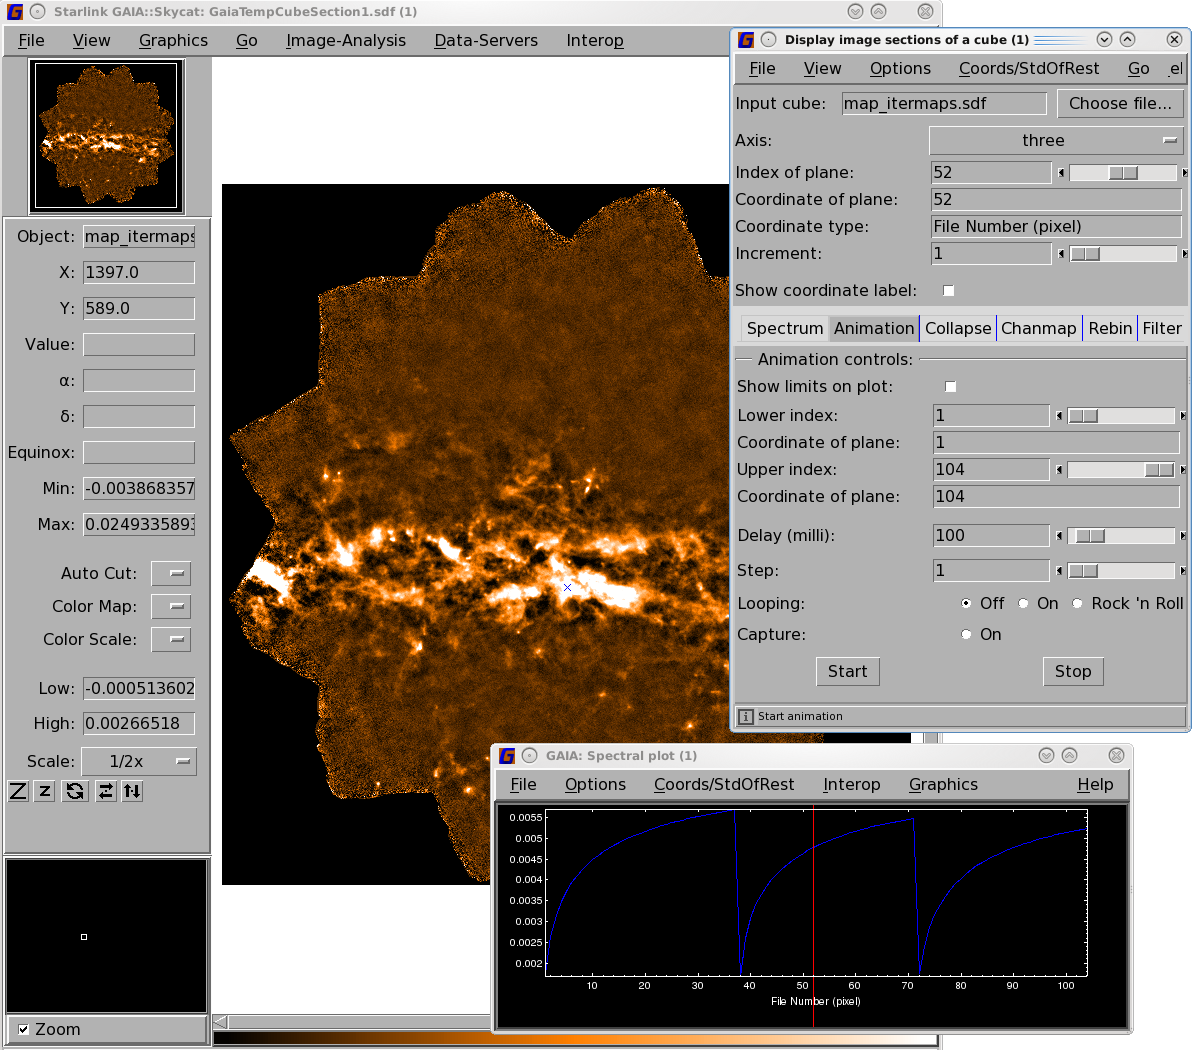
\includegraphics[width=0.95\textwidth]{sc21_itermaps_anim}
\end{minipage}
\hspace{0.3cm}
\begin{minipage}[c]{0.29\linewidth}
The output map \file{map\_itermaps} can be opened with \gaia. The data used
in this example is the Galactic map reduced in
\cref{Section}{sec:bright_ex}{\file{dimmconfig\_bright\_extended.lis}}. The
Spectral plot window shows the value for a single pixel and the three
chunks are easily identified. You can select the \gaiathing{Animation} tab
in the \gaiathing{Display image sections} window and click
\gaiathing{Start} to loop through the itermaps for each iteration.  The
`movie' will appear in the main \gaia\ window.
\end{minipage}
\minipageclear

\vspace{0.7cm}

\begin{minipage}[c]{0.65\linewidth}
\centering
\hspace{0.5mm}
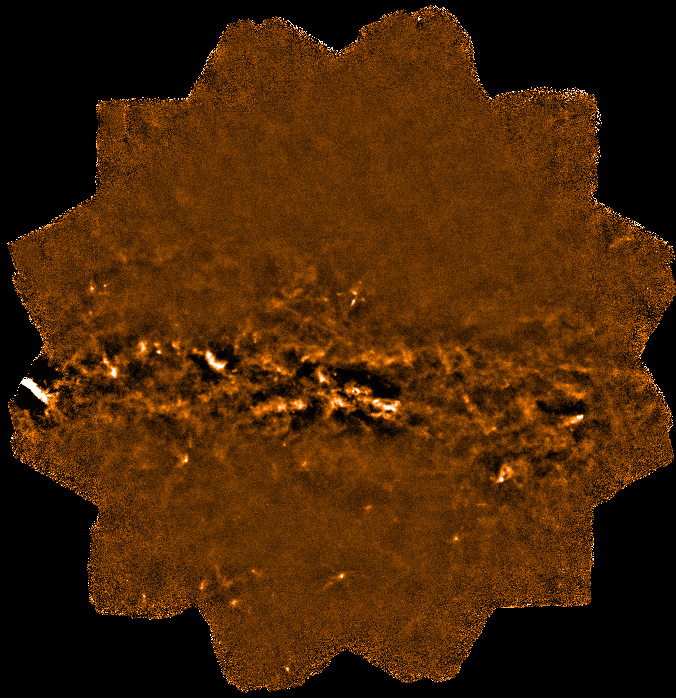
\includegraphics[width=3cm, ]{sc21_iter1}
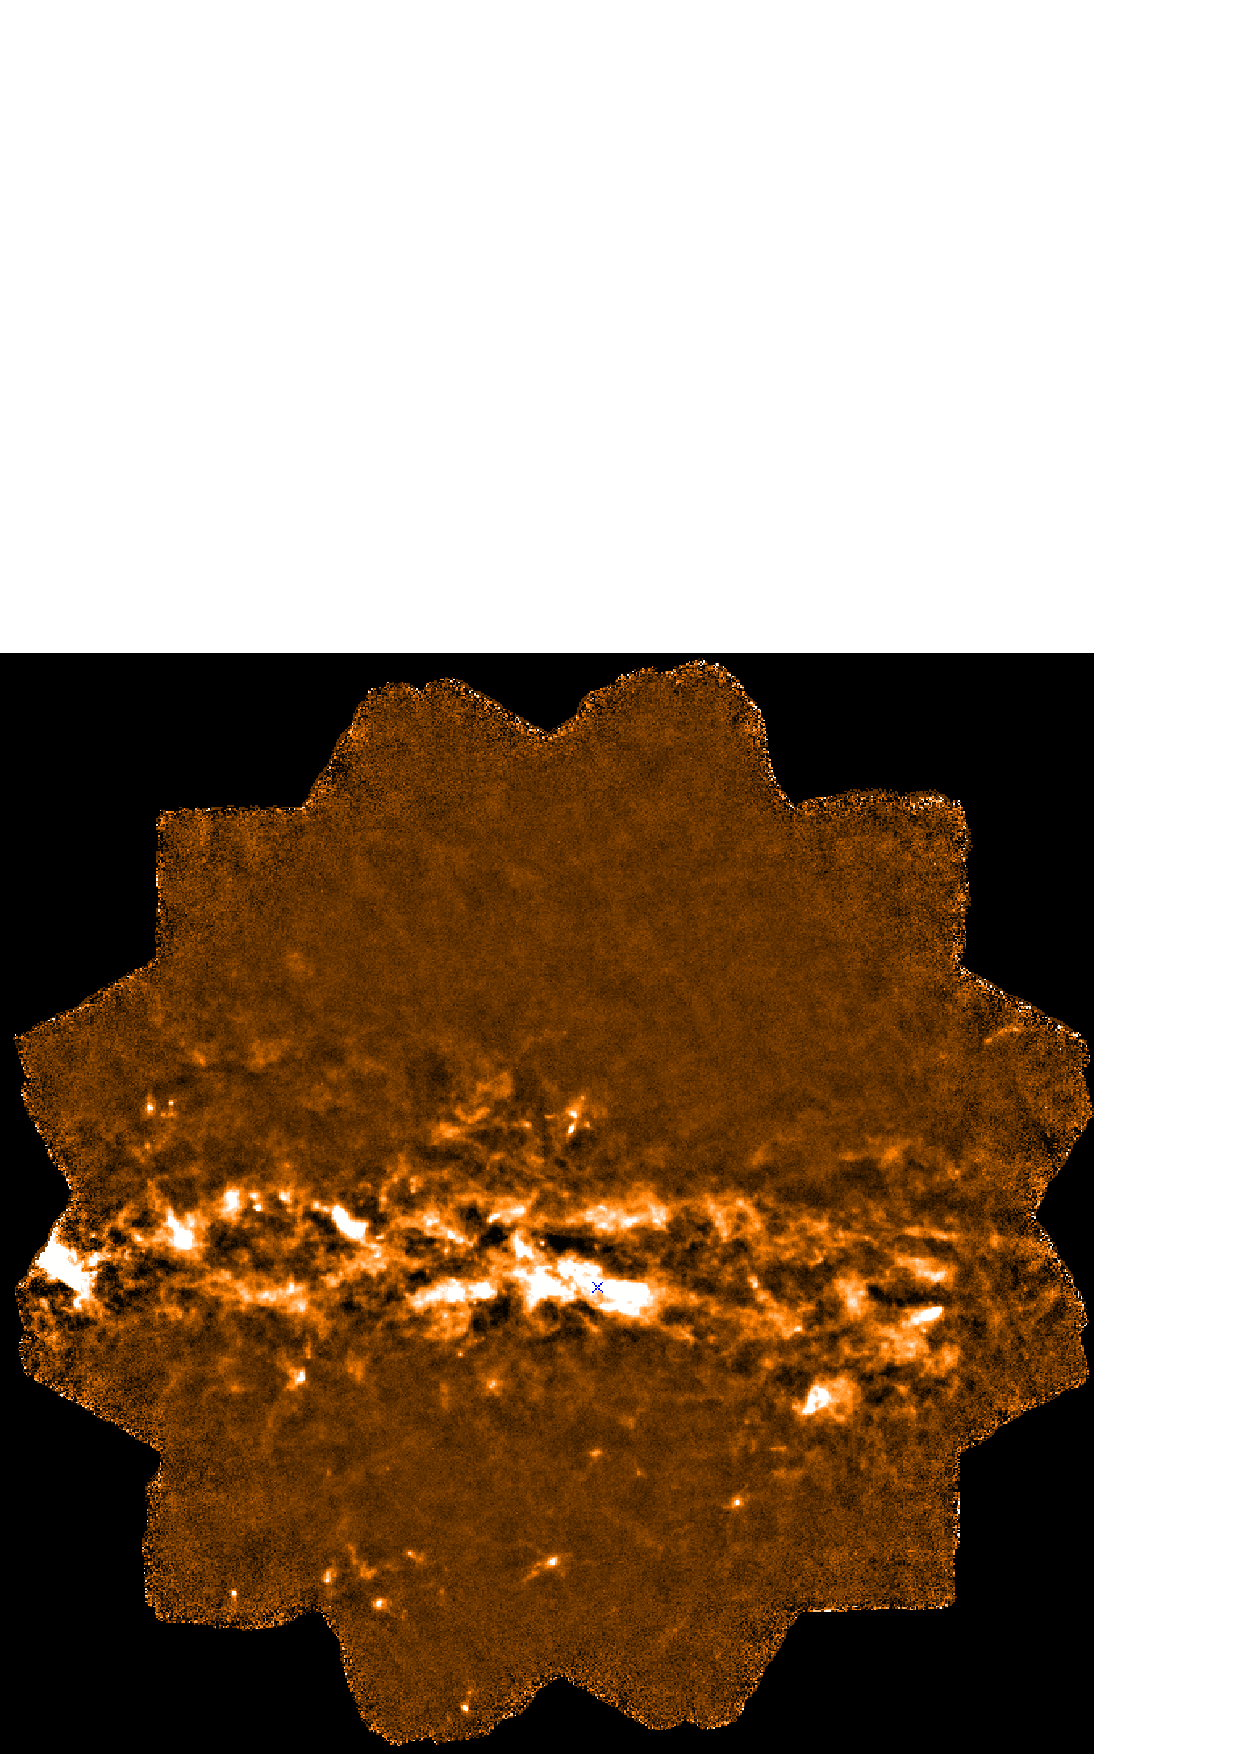
\includegraphics[width=3cm, ]{sc21_iter2}
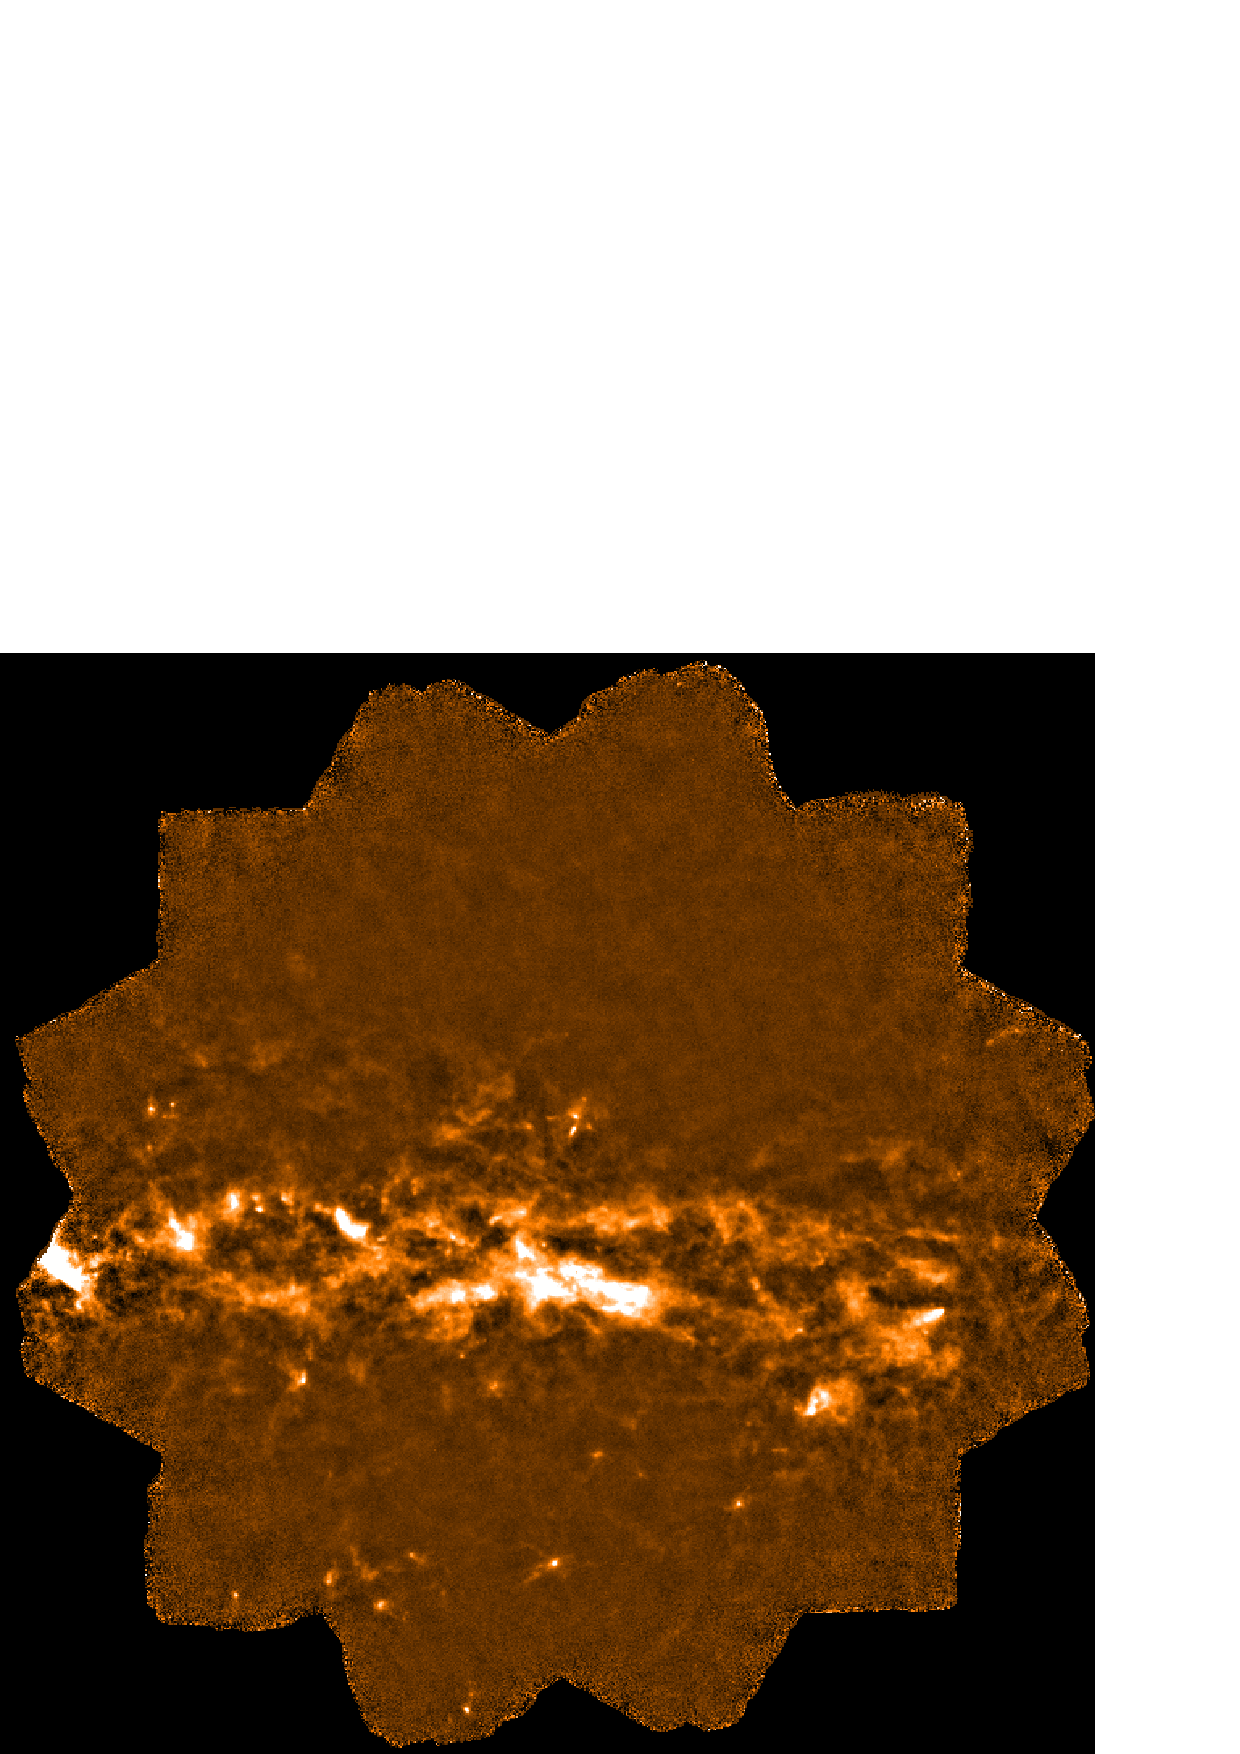
\includegraphics[width=3cm, ]{sc21_iter31}
\vspace{0.2cm}
\end{minipage}
\hspace{0.3cm}
\begin{minipage}[c]{0.29\linewidth}
These windows show the itermaps map at 1, 10, and 30 iterations. A
specific iteration can be selected using the \gaiathing{Index of plane}
slider on the \gaiathing{Display image sections} window.
\vspace{0.2cm}
\end{minipage}
\minipageclear
\end{fmpage}
\end{center}
\caption[View maps for each iteration]{
  \small Example using the \smurf\ command \stackframes\ and
  \gaia\ to view the `itermap' for each iteration.
}
\label{fig:stack}
\end{figure}


\begin{terminalv}
% gaia 850map.more.smurf.shortmaps
\end{terminalv}

You can view the shortmaps and itermaps more
conveniently by stacking them into a single cube using the \smurf\
command \stackframes. This cube can then be viewed as a
`movie' with \gaia, using the animation option to loop through the
itermaps. See \cref{Figure}{fig:stack}{the box above} for instructions.
\newline\newline
\textbf{exportmodel}\\
This parameter has been discussed in
\cref{Section}{sec:export}{Exporting individual models} and allowed
you to see the model that was fit for each component specified by the
\param{modelorder} parameter.

\section{\xlabel{filt}Large-scale filtering}
\label{sec:filt}

Some of the most important parameters to experiment with are the
filtering options. By default the low-pass filter is applied once
during the pre-processing stage and is turned off for the iterative
steps. The high-pass filter is only specified during the iterative
steps and its selected value is crucial for maps containing extended
emission.

The maximum spatial scale of structure that can be recovered by the
map-maker is determined by the scanning speed and frequency cut
applied to the data:

\begin{equation}
\frac{\textrm{speed}[\prime\prime / \textrm{s}]}{\textrm{frequency
    cut}[\textrm{Hz}]}=\textrm{scale size}[\prime\prime]
\end{equation}

The filtering options set in \file{dimmconfig.lis} are:

\param{450.flt.filt\_edge\_largescale~=~600} \\
\param{850.flt.filt\_edge\_largescale~=~300}.

To make your life easier, these parameters allow you to specify the
filter limits in terms of spatial scale in arcsecs---in this case
300\,arcsec at 850\,$\mu$m and 600\,arcsec at 450\,$\mu$m. For example,
at 850\,$\mu$m, recovering scales of 300\,arcsec at a scan speed of
600\,arcsec/sec (default for a 1 degree \textsc{pong}) corresponds to
a frequency of 2\,Hz.

Choosing a high-pass filter is especially important for the recovery
of extended emission. The \file{dimmconfig\_bright\_extended.lis}
recipe sets \param{flt.filt\_edge\_largescale~=~480} (i.e. both 450
and 850\,$\mu$m). Be aware that increasing filtering scales decreases
the flatness of your background. A compromise must be made between
extended structure and the flatness of your map. See
\cref{Figure}{fig:fltcompare}{the figure below} for an illustration of
the effect of \param{flt.filt\_edge\_largescale} on your map.

The scanning speeds are fixed for a given observing mode; you can find
out the speed at which your data were taken from the
\texttt{SCAN\_VEL} keyword in the FITS header (see
\cref{Section}{sec:fitsheader}{Headers and file structure}).

%\pagebreak[4]
\textbf{Flattening the background}\\*
There is an option to reduce the noise in your background introduced by
setting a high value for the large-scale filter. The parameter
\param{FLT.FILT\_EDGE\_LARGESCALE\_LAST} filters the regions outside
your \model{AST} mask on a shorter scale for the last iteration only,
thereby producing a much flatter background.

Note that the variances stored in the final map are from the penultimate
iteration to avoid having artificially reduced values.


\begin{figure}
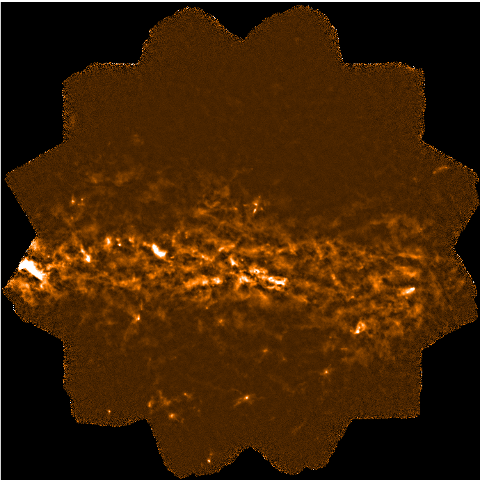
\includegraphics[width=0.46\linewidth]{sc21_brex_19}
\hspace{7mm}
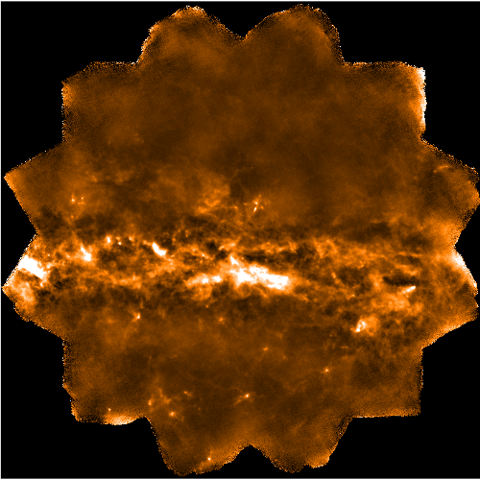
\includegraphics[width=0.46\linewidth]{sc21_brex_18}
\caption[Illustrating the effects of high-pass filtering]{
  Highlighting the effects of high-pass filtering on your map.
  \textbf{(Left)} Map made with \param{850.flt.filt\_edge\_largescale~=~300}.
  \textbf{(Right)} Map made with \param{850.flt.filt\_edge\_largescale~=~1000}.
  All other configuration parameters remain the same.\label{fig:fltcompare}
}
\end{figure}


\section{\xlabel{fitcom}Fitting COM for each sub-array}
\label{sec:fitcom}

A useful option to improve the flatness of your maps is to fit the
\model{COM} model independently for each sub-array. This is
particularly effective if you find you have one sub-array noisier than
the others.

This comes with the warning however that you will lose information on
any scales larger than the area covered by a single sub-array. It is
therefore not recommended if you have very large-scale extended
structure.

To initialise this option set \param{com.perarray~=~1}.


\section{\xlabel{noibox}Flagging bad data}
\label{sec:noibox}

It is possible to down-weight data that have higher noise by setting
the parameter \param{noi.box\_size}. If this is set (i.e. non-zero),
then the length of time over which the noise is determined can be
specified in time samples (positive values) or seconds (negative
values). By default this is set to zero and the whole time stream is
used giving a single variance for each bolometer. This variance is
used to weight the data for subsequent iterations, hence more finely
estimated noise levels are preferable.

The parameter \param{noi.box\_size} helps remove `scuffs' or other
noise artefacts you might see in your error map due to a sub-array (or
arrays) temporarily jumping to a higher noise state. The default file
has \param{noi.box\_size = - 15} (i.e. half a sub-scan). As the
value tends to $-$1 (one second) we find some of the source signal being
down-weighted. Higher than this $-$15 value and the map-maker becomes
less sensitive to the higher noise states.

Other parameters you may want to try include \param{flagfast} and
\param{flagslow}. You may find that setting \param{flagfast} to less
than the default of 1000\,arcsec/sec will help reduce the effect of any
`smearing' of sources (and of noise) in maps, while setting
\param{flagslow} greater than the default of 300\,arcsec/sec helps to
flatten the edges of maps. To determine reasonable values for your
 dataset you should do \jcmtstate\ and view the scan speed using
\topcat. See \cref{Section}{sec:scan}{Displaying scan patterns} for
details.


\section{\xlabel{mask}Masking options}
\label{sec:mask}

The \model{AST}, \model{FLT} and \model{COM} models each have a
number of masking options. The ones common to each model are listed
below.  Replace the \param{xxx} with the relevant model name.

\begin{table}[h!]
\begin{tabular}{p{3.5cm}p{10.5cm}}
\param{xxx.zero\_circle}  & Defines a circular mask of a specified radius.
                            Used for compact sources.\\
\param{xxx.zero\_lowhits} & Defines a mask by the number of data samples
                            in a pixel. This means that spurious
			    regions of emission at the edges of the
			    map, where exposure time is low, are not
			    included in the mask.\\
\param{xxx.zero\_snr}     & Creates a mask after each iteration based on
                            the S/N in each pixel.\\
\param{xxx.zero\_snrlo}   & Allows the mask created by \param{xxx.zero\_snr}
                            to expand down to a specified S/N.\\
\param{xxx.zero\_union}   & Controls how the masks are combined. For instance,
                            if two masks are defined, one from lowhits and one
                            from the signal-to-noise.\\
\param{xxx.zero\_freeze}  & Prevents the masking from changing after a
                            specified number of iterations.\\
\end{tabular}
\end{table}


Masking comes with different restrictions and sensitivities depending on the
model in question.

\begin{description}
\item[AST mask]
\model{AST} masking is always used where emission is expected. The map
is constrained to zero at all points outside the masked region and the
\model{AST} model is estimated based only on data inside the mask.

\item[FLT mask]
\model{FLT} masking is used to omit bright sources from the estimate
of the low-frequency background subtracted from the residuals on each
iteration. This can help prevent ringing in the final map. S/N based
\model{FLT} masking cannot be used on the first iteration and
\model{FLT} masking should be used sparingly to aid convergence (it
is limited to the first two iterations by default with
\param{flt.zero\_niter~=~2}).

\item[COM mask]
\model{COM} masking is used to omit very bright sources from the
estimate of the common-mode signal, this can prevent sources being
rejected due to their dissimilarity to the common-mode. S/N based
\model{COM} masking cannot be used on the first iteration and the
mask should always be small.

\item[Signal-to-noise masking]
Masking based on the signal-to-noise ratio is used for both the \model{AST}
and \model{FLT} models for extended emission. The recipe
\file{dimmconfig\_bright\_extended.lis} sets \param{ast.zero\_snr}
to 5 and \param{ast.zero\_snr} to 3. Setting \param{ast.zero\_snr}
too low can cause noise spikes to be interpreted as signal so
\param{ast.zero\_snrlo} is used which allows the mask to only grow it
it includes pixels with the specified S/N. This typically improves the
resulting map so it is worth experimenting with. Note that \model{AST}
masking is not applied on the final iteration to allow data outside
the mask to remain in the final map.

The bright-extended recipe also sets \param{ast.skip} to 5. This
means the \model{AST} model is not determined at all for the first
five iterations. This used in conjunction with \model{FLT} masking
which is performed in these \model{AST}-free iterations.

\item[External masking]
An alternative to S/N masking is to supply an external mask using the
\param{REF} parameter. Setting the parameter
\param{ast.zero\_snr\_fwhm} allows you to automate this step for a
specific case. Here, the map-maker is run once, then the mask
generated by \param{ast.zero\_snr} is smoothed by a Gaussian (of
`FWHM' arcsecs) and the map-maker is re-run with this smoothed mask
supplied as an external mask. You can supply your own external mask
however by following the instructions in the next section.

\item[Combining masks]
Multiple masks are combined according to the \param{xxx.zero\_union}
parameter. If this parameter is true (i.e. non-zero) then the two masks
will be combined to act as one large mask (the union of the individual
masks). Hence a pixel will be flagged/masked if it falls within either
mask (rather than being required to fall in both). The alternative is
a false (i.e. zero) value; this means that only pixels that fall into
both masks independently will be flagged/masked. In this case only the
intersection of the masks is considered the final masked area.

For example, if you find an S/N mask allow bright regions to develop
towards the edges of your map, you can force these to zero by using
the intersection of the S/N mask with a lowhits mask.

\item[Freezing masks]
The \param{ast.zero\_snr} parameters stop the masks from growing
(or changing) indefinitely. After the first few iterations the mask
have essentially reached their maximum scale but a few edge pixels
oscillate in and out of the masks. This results in a significant enough
change in the \param{maptol} that convergence is never achieved. The
final maps however are essentially identical.
\end{description}

\section{\xlabel{maskbe}Supplying an external mask}
\label{sec:maskbe}

As an S/N mask is redetermined after each iteration it changes with the map
 which can sometimes cause convergence problems. The mask
will also depend on the amount of data going into the map and the
pixel size. A fixed externally supplied mask  can get around these problems.

The sequence below is a summary of the procedure for generating and
supplying an external mask. In this example the mask is generated from
the map produced by an initial run through the map-maker.
Alternatively maps from other observatories can be used.

These steps are followed in the example in
\cref{Section}{sec:bright_ex}{Extended galactic sources}.

\begin{aligndesc}
\item[Step~1] Generate a map covering your region. This may be by
  simply running the map-maker on your data as shown below.
\begin{terminalv}
% makemap in='s8*.sdf' out=850map method=iterate \
config='"^dimmconfig_bright_extended.lis"'
\end{terminalv}
The alternative is to access a map from a different dataset or even a
different telescope, e.g. a map downloaded from the Herschel Science
Archive. For instructions on converting from FITS to NDF see
\cref{Appendix}{app:fits}{Convert format from FITS to NDF}.\\

\item[Step 2] Make a signal-to-noise map using the \Kappa\ command
  \makesnr.
\begin{terminalv}
% makesnr 850map 850map_snr
\end{terminalv}

\item[Step 3] This S/N map is thresholded to set everything below
  3$\sigma$ to 0 and everything above to 1.
\begin{terminalv}
% thresh 850map_snr 850map_mask thrlo=3 newlo=0 thrhi=3 newhi=1
\end{terminalv}
This generates a mask which has an unrealistic hard 3$\sigma$
cut-off. Step 4 is performed to smooth the the edges of your mask.

\item[Step 4] The thresholded map is smoothed with a Gaussian filter
  of FWHM of 5 pixels (=\,20\,arcsec). Then it is again thresholded,
  this time keeping everything above 5\,\% of the 0 level as the mask
  and setting the rest to \texttt{bad}.
\begin{terminalv}
% gausmooth 850map_mask 850map_mask_sm fwhm=5
% thresh 850map_mask_sm 850map_mask_zm thrlo=0.05 newlo=bad \
  thrhi=0.05 newhi=1
\end{terminalv}

\item[Step 5] Finally the map is re-made with this mask supplied as an
  external file. Notice that the extra parameters required to pick up
  this external mask are being appended to the configuration file on
  the command line rather than editing the file itself.
\begin{terminalv}
% makemap in='s8*.sdf' out=850map_zm method=iterate \
  config='"^dimmconfig_bright_extended.lis,ast.zero_mask=1,\
  ast.zero_snr=0"' ref=850map_mask_zm
\end{terminalv}

\end{aligndesc}

\section{\xlabel{skyloop}Skyloop}
\label{sec:skyloop}

\starfig{sc21_skyloop}{}{width=0.55\linewidth}{fig:skyloop}{
  Illustration of the \task{skyloop} approach}{
  Illustration of the \task{skyloop} approach
  to map-making compared with the standard map-maker.
}

Traditionally, the map-maker divides a non-contiguous sequence of time
series data into chunks. It processes each chuck independently
before co-adding them as a final step in the the reduction---see
\cref{Figure}{fig:skyloop}{the figure below}.

This means for each chunk the map-maker has to start from scratch
determining the \model{AST} model and the benefit of long integration
times spent building up the signal is lost. Recipes which use
signal-to-noise masks especially suffer from this approach as the
signal-to-noise in each individual chunk can remain low and fainter
extended structure is not recovered.

This new \skyloop\ command runs \makemap\ multiple times
performing just a single iteration on each occasion. It starts by
performing a single iteration of \task{makemap} from which a final
co-added map is generated. This map is then supplied as an initial
estimate of the sky for the next loop through \task{makemap}. On
this next iteration, the initial sky estimate is subtracted from the
cleaned time-series data and the \model{COM}, \model{GAI},
\model{FLT}, \model{EXT} models are subtracted. This produces a new
model of the sky (from the current iteration) to which the sky
estimate (from the previous iteration) is then added. In this way the
signal from all of the chunks is built up over the iterations and is
all included in the final map estimate when convergence is reached.




Be aware that \task{skyloop} uses a lot of disk space. Setting
environment variable \envvar{STAR\_TEMP} to a suitable location
before you start will prevent \task{skyloop} from crashing
if you run out of temporary storage space.
\begin{terminalv}
% setenv STAR_TEMP .
\end{terminalv}
\task{skyloop} can then called in the same way as \makemap, with
 a configuration file specified on the command line.
\begin{terminalv}
% skyloop in=^myfiles.lis out=map_skyloop config=^dimmconfig_bright_extended.lis \
LOGFILE=skyloop.log ILEVEL=ATASK GLEVEL=debug
\end{terminalv}

\section{Troubleshooting}
Two troubleshooting configuration files are provided which target specific
problems during reduction.

\begin{itemize}

\item \file{dimmconfig\_fix\_blobs.lis}\\
The parameters in this file are designed to prevent smooth blobs of bright
emission appearing in the final map. These parameters are explained below.

\begin{itemize}[nolistsep]
\item \param{flt.filt\_order~=~4} to set a 4th-order Butterworth
  filter for the \model{FLT} model.

  \item \param{flt.ring\_box1~=~0.5} uses a filter to identify and flag
  time-samples that are ringing after the \model{FLT} model. This only starts
  after the \param{ast.skip} iterations (in bright\_extended) have completed.
  \item \param{com.sig\_limit~=~5} flags time slices where the
  \model{COM} model is very different from the average for each
  sub-array. This should only be used when \param{flt.filt\_order} is set. If
  it is set too stringently it can throw out a lot of data so modify with
  caution. We would not recommend lower than $\sim$2.
\end{itemize}
\end{itemize}

\begin{itemize}
\item \file{dimmconfig\_fix\_convergence.lis}\\
The parameters in this file are designed to help a map which will not
converge within a reasonable number of iterations. The parameters are
listed below.
\begin{itemize}[nolistsep]
\item \param{com.freeze\_flags~=~10} stops flags generated by the \model{COM}
model determination from changing after the first ten iterations.
\item \param{ast.zero\_freeze~=~10}
\item \param{flt.zero\_freeze~=~10}
\item \param{com.zero\_freeze~=~10}
\end{itemize}
These \param{xxx.zero\_freeze} parameters stop the respective masks
growing after ten iterations. By this stage they have essentially reached
their final shape and it is only a few pixels around the edge of the masks
which oscillate in and out and prevent convergence.
\end{itemize}

These recipes can either be called directly by an external configuration
file---see \cref{Section}{sec:problem}{Solving configuration-file problems}
or the parameters can be included (and edited) in your personalised
configuration file.

\begin{table}[b]
\begin{center}
\begin{tabular}{|p{5cm}|p{10.5cm}|}
\hline
\textbf{PROBLEM} & \textbf{POSSIBLE SOLUTION}\\
\hline
I have blobs in my map that look like big thumbprints. & Try using
\file{dimmconfig\_fix\_blobs.lis} in addition to your current configuration
file.  Note that this sets \param{com.sig\_limit~=~5} which is somewhat
conservative. You can experiment by lowering this, but we would not recommend
lower than $\sim$2 before you lose too many samples.

In addition, check you are not using \param{flt.notfirst~=~1} as this
can make blobs worse.\\
\hline
I want to recover more extended structure. & There is a trade off
between extended emission and noise in your map. If you are willing to
accept more low frequency noise you can increase the filter scale with
\param{flt.filt\_edge\_largescale}. The default is 480\,arcsec but you
could try 600\,arcsec. To cosmetically reduce the increased background
noise you can set \param{flt.filt\_edge\_largescale\_last~=~200}. This
sets the background filtering to 200\,arcsec for the final iteration
only, though you can go as low as you want with it. \\
\hline
I want a flatter background.  & Try \param{com.perarray~=~1}, although
be aware this will lose structure on scales larger than a sub-array. In
conjunction with \param{com.perarray~=~1} you can also use the
\param{ast.skip~=~8} parameter. This makes a map without subtracting an
\param{AST} model for the first eight iterations. If you are chasing
extended emission see the point above. For a more uniform background set
\param{flt.filt\_edge\_largescale\_last} to a small value to get harsh
filtering on your final iteration.\\
\hline
I have linear striations in my map making my background look
scratchy.& Try setting \param{com.corr\_abstol~=~0.8} [default=0.2].
This rejects more bolometers with deviant common-mode signals.
However, as more bolometers are removed there are fewer data available
for your final map, resulting in higher noise.\\
\hline
My map will not converge.& Try including \file{dimmconfig\_fix\_convergence.lis}
n addition to your configuration file. These parameters are to stop the
masks from changing after ten iterations.\\
\hline
\end{tabular}
\end{center}
\end{table}






\chapter{\xlabel{Examples}Examples of Different Reductions}
\label{sec:eg}

\section{\xlabel{Cosmology}Deep point-source maps}
\label{sec:cosmology}

The science goal of many extra-galactic SCUBA-2 observations is to
detect unresolved point sources. In the examples below we work through the
reduction of just such an extra-galactic field, A1835.

Most extra-galactic objects are on average only slightly brighter than
the confusion limit---the fluctuations of the background sky
brightness due to multiple super-imposed, unresolved sources within
the telescope beam, below which individual sources cannot be detected.
It is likely that any sources in the map will be at best, only a few
standard deviations brighter than the noise in the map (caused by a
combination of instrumental noise and source confusion).

\subsection{Example 1 -- The simple reduction}
The basic reduction method for maps like these follow two main
steps---running the data through the map-maker using the
\file{dimmconfig\_blank\_field.lis} recipe (see
\cref{Section}{sec:config}{Specialised configuration files}). Then
applying the \picard\ \drrecipe{SCUBA2\_MATCHED\_FILTER} recipe (see
\cref{Section}{sec:mf}{Point-source extraction}).
\\ \\
\textbf{Step 1: Run the map-maker}\\
In this example the raw data are stored locally in a directory called
\file{data}. We have three observations (\#13, \#18, \#21) of the field
which we will reduced independently.

\begin{terminalv}
% makemap data/s8*00013_00\*.sdf cosmo1 method=iterate \
config=^$STARLINK_DIR/share/smurf/dimmconfig_blank_field.lis

% makemap data/s8*00018_00\*.sdf cosmo2 method=iterate \
config=^$STARLINK_DIR/share/smurf/dimmconfig_blank_field.lis

% makemap data/s8*00021_00\*.sdf cosmo3 method=iterate \
config=^$STARLINK_DIR/share/smurf/dimmconfig_blank_field.lis

\end{terminalv}

\textbf{Step 2: Combine the maps}\\
These three maps are then combined using the \textsc{Picard} recipe
\xref{\drrecipe{MOSAIC\_JCMT\_IMAGES}}{sun265}{MOSAIC_JCMT_IMAGES}. In
this case we accept the default of \wcsmosaic\ mosaicking and
nearest-neighbour pixel spreading and so do not supply a parameter
file.
\begin{terminalv}
% picard MOSAIC_JCMT_IMAGES cosmo*.sdf
\end{terminalv}
The output map, \file{cosmo3\_mos.sdf} (named for the last input file
appended by \_mos), is shown in the left-hand panel of
\cref{Figure}{fig:cosmomap}{the figure below}. The advantage of using the
\textsc{Picard} recipe over standalone \Kappa\ commands is that the exposure
time is also propagated correctly to the output mosaic (it is stored
in the \texttt{MORE.SMURF.EXP\_TIME} extension).
\\

\begin{figure}
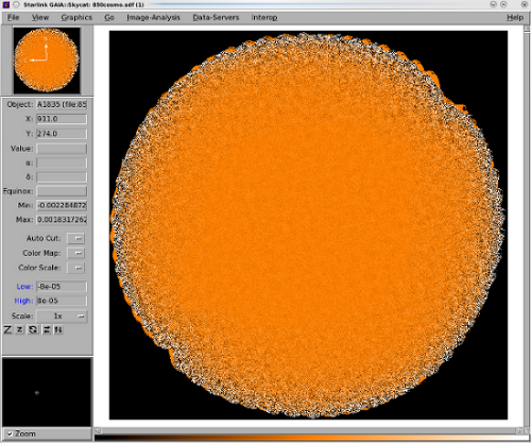
\includegraphics[width=0.48\linewidth]{sc21_850cosmo_bf}
\hspace{2mm}
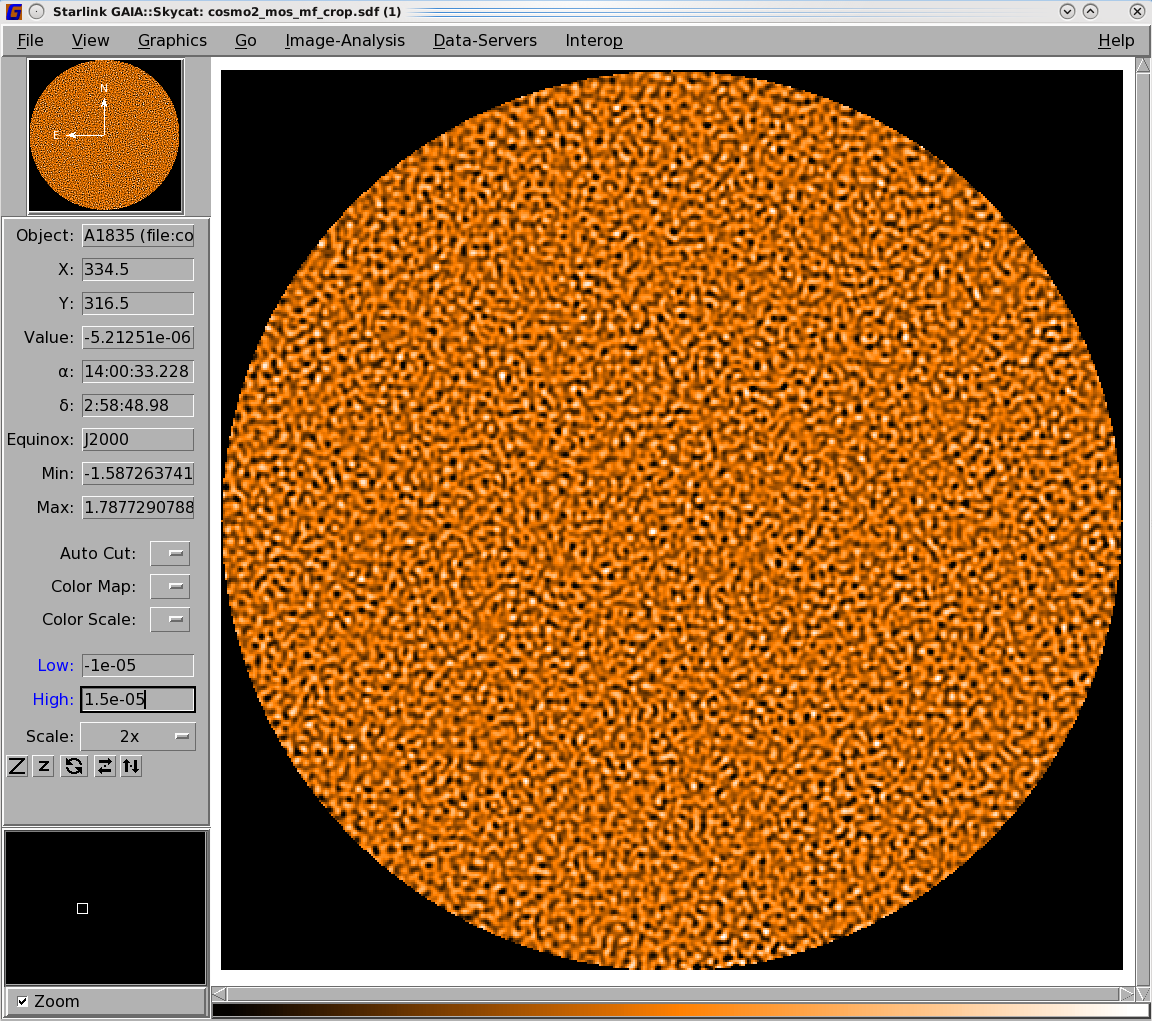
\includegraphics[width=0.48\linewidth]{sc21_850cosmo_mf_crop}
\caption[Cosmology field with the matched filter applied]{
  Reduced \textsc{pong} maps of cosmology field A1835. \textbf{Left:}
  Map reduced with \file{dimmconfig\_blank\_field.lis}.
  \textbf{Right:} Map on the left after the matched filter has been
  applied and it has been cropped.\label{fig:cosmomap}
}
\end{figure}

\textbf{Step 3: Apply the matched filter}\\
In order to optimally find sources that are the size of the telescope
beam, we apply the matched filter recipe, namely
\xref{\drrecipe{SCUBA2\_MATCHED\_FILTER}}{sun265}{SCUBA2_MATCHED_FILTER}.
We create a simple parameter file called \file{smooth.ini}:

\begin{terminalv}
[SCUBA2_MATCHED_FILTER]
SMOOTH_FWHM = 15
\end{terminalv}
where \param{SMOOTH\_FWHM~=~15} indicates that the background should be
estimated by first smoothing the map and PSF with a 15-arcsec FWHM
Gaussian. Next, the recipe is executed as follows:
%
\begin{terminalv}
% picard -recpars smooth.ini SCUBA2_MATCHED_FILTER cosmo2_mos.sdf
\end{terminalv}
%
The output of this operation is a smoothed image called
\file{cosmo3\_mos\_mf.sdf} and a cropped version is shown in the
right-hand panel of \cref{Figure}{fig:cosmomap}{figure above}. You can immediately
see the contrast to the left-hand panel which is the output from the
map-maker. A number of signal peaks now emerge as possible sources.
\\ \\
\textbf{Step 4: Crop the map}\\
Next we shall crop the map to remove the noisy edges,
in this case to a 900-arcsec radius circle. The output file will be named
\file{cosmo2\_mos\_mf\_crop.sdf}.
\begin{terminalv}
% picard CROP_JCMT_IMAGES cosmo3_mos_mf.sdf

\end{terminalv}

\starfig{sc21_850cosmo_mf_crop_snr}{}{width=0.6\linewidth}{fig:snrmask}{
  S/N map of a cosmology field}{
  Signal-to-noise map made using the \Kappa\ command \makesnr.
  The map has been scaled from 0 to $+$3.
}

\textbf{Step 5: Make an S/N map}\\
Finally, we need to find sources. The filtered map contains a
VARIANCE component, so it is easy to produce a S/N map using the
\textsc{Kappa} task \makesnr:
\begin{terminalv}
% makesnr cosmo2_mos_mf_crop cosmo2_mos_mf_crop_snr
\end{terminalv}

The resulting map, \file{cosmo2\_mos\_mf\_snr}, is shown in
\cref{Figure}{fig:snrmask}{the signal-to-noise image}. Compared with the
matched filter map the
edges no longer appear as noisy because they have been down-weighted
by the larger noise values where there were less data.
\\ \\
\textbf{Step 6: Identify sources}\\
The basic procedure for identifying sources would be to locate peaks
above some threshold S/N. The S/N image above shows peaks that are
likely to be real sources. For a start, a source appears where
expected at the 0,0 position.

But how can we check if these sources are real?
\begin{itemize}

\item One option is to split your data into mutually exclusive subsets
  and produce independent maps. Are the highest S/N peaks detected in each of
  them?
\item A second test is to compare the number of \emph{negative} peaks above
  a given S/N with the number of \emph{positive} peaks.
\end{itemize}

\subsection{Example 2 -- Advanced pipeline method}
\label{sec:jk}

Although this method is considerably simpler to execute, the products
have undergone more advanced processing than the manual method just
given. The pipeline is particularly recommended for this recipe due to
its extra analysis steps.

\textbf{Step 1: Create input file}\\
Create an file with the names of all the files you wish to process (e.g.
\file{myfiles.lis})
\\ \\
\textbf{Step 2: Run the pipeline}\\
The pipeline must first be initiated for the wavelength you are
working on. In the case below this is 850\,$\mu$m. Note that the date
does not \emph{have} to be specified when initialising the pipeline.
The pipeline is run using the
\xref{\drrecipe{REDUCE\_SCAN\_FAINT\_POINT\_SOURCES\_JACKKNIFE}}{sun264}{REDUCE_SCAN_FAINT_POINT_SOURCES_JACKKNIFE}
recipe; this uses \file{dimmconfig\_blank\_field.lis} as the
configuration file. If you wish to provide an alternative file you
will need to put the name of the new configuration file in a recipe
parameter file.  See \cref{Section}{sec:pipe}{The SCUBA-2 Pipeline}
for details.
\begin{terminalv}
% oracdr_scuba2_850 -cwd YYYYMMDD
% oracdr -loop file -files myfiles.lis -nodisplay \
-log sf FAINT_POINT_SOURCES_JACKKNIFE
\end{terminalv}

You substitute the required date for \texttt{YYYYMMDD}.
The pipeline will write out a large number of files with the following
suffices.

\begin{aligndesc}
\item[\file{sYYYYMMDD*\_fmos}]
The map for each observation

\item[\file{sYYYYMMDD*\_mappsf}] The map for each observation with an
  artificial point source added at the map centre

\item[\file{gsYYYYMMD*\_wmos}] The co-add of all the \file{\_fmos}
  files

\item[\file{gsYYYYMMD*\_whiten}] The whitened version of \file{\_wmos}

\item[\file{gsYYYYMMD*\_cal}] The calibrated version of
  \file{\_whiten}

\item[\file{gsYYYYMMD*\_mf}] The matched-filtered version of
  \file{\_cal}
\end{aligndesc}

\drrecipe{FAINT\_POINT\_SOURCES\_JACKKNIFE} is a recipe designed to
process blank field/extra-galactic data. The recipe uses a
\htmladdnormallink{jack-knife}{http://en.wikipedia.org/wiki/Jackknife_resampling}
method to remove low-spatial frequency noise and generate a matched
filter output map.

The recipe processes each observation twice, a standard reduction
first, then a re-run with a fake point source added to the time
series. This produces a co-added signal map (\file{\_wmos}) and a
coadded PSF map (\file{\_mappsf}).

\begin{tip}
The recipe name \drrecipe{FAINT\_POINT\_SOURCES\_JACKKNIFE} can be used
interchangably with  \drrecipe{REDUCE\_SCAN\_FAINT\_POINT\_SOURCES\_JACKKNIFE}.
\end{tip}


After the map-maker has completed, the recipe will call
\xref{\drrecipe{SCUBA2\_JACKKNIFE}}{sun265}{SCUBA2_JACKKNIFE}. This
routine divides the observations into two groups (odd and even) which
are co-added and then subtracted to create a jack-knife map. This map
contains only noise with no contribution from astronomical signal. The
angular power spectrum of this map is then used to estimate and remove
the residual 1/\emph{f} noise from the signal map and the PSF map;
this is the whitening step. The whitened jack-knife map is run through
\xref{\drrecipe{SCUBA2\_MATCHED\_FILTER}}{sun265}{SCUBA2_MATCHED_FILTER}
using the whitened PSF map as the PSF input. It is this matched filter
map which will be of most interest to users.

See \pipelinesun\ for more information on
\drrecipe{REDUCE\_SCAN\_FAINT\_POINT\_SOURCES\_JACKKNIFE} and all other pipeline
recipes.
\\ \\
\textbf{Step 3: (Optional) Re-run \drrecipe{SCUBA2\_JACKKNIFE}}\\
You may wish to run the \drrecipe{SCUBA2\_JACKKNIFE} step again
independently from the pipeline. If your final map does not look as
expected you might first examine the individual mosaics from the
pipeline (\file{\_fmos}), one of these observations might show visible
artefacts that you wish to exclude from the co-add. The size of the
region in the jack-knife image which is used to do the whitening step
is determined automatically, but the method may fail if the box is too
small.

If you decide to re-run this step you first co-add all the
\file{\_mappsf} files to create a coadded PSF using the \picard\ recipe
\xref{\drrecipe{MOSAIC\_JCMT\_IMAGES}}{sun265}{MOSAIC_JCMT_IMAGES}.
\begin{terminalv}
% picard MOSAIC_JCMT_IMAGES *_mappsf
\end{terminalv}
Next create a parameter file (\file{recpars.lis}) for the jack-knife
recipe (\drrecipe{SCUBA2\_JACKKNIFE}) containing the following lines.
\begin{terminalv}
[SCUBA2_JACKKNIFE]
PSF_MATCHFILTER = <name_of_above_coadded_PSF>.sdf
\end{terminalv}
Another option for this parameter file is \param{WHITEN\_BOX} to set the
size of the region used to calculate the angular power spectrum.
Finally run \drrecipe{SCUBA2\_JACKKNIFE}.
\begin{terminalv}
% picard -log sf -nodisplay -recpars recpars.lis SCUBA2_JACKKNIFE *fmos.sdf
\end{terminalv}
This will create files beginning with \file{pgYYYMMDD}$\ldots$ that
should have the same suffices as above: \file{\_wmos},
\file{\_whiten}, \file{\_cal}, and \file{\_mf}.



\section{\xlabel{Galactic}Extended galactic sources}
\label{sec:bright_ex}

This example is concerned with recovering bright extended emission.
The signal from extended emission varies slowly as seen by the array
passing over it. It thus appears at lower frequencies in the power
spectrum and complicates the high-pass filter selection. Too harsh a
filter will make flat maps but any extended emission will have been
removed in doing so.
\\ \\
\textbf{Step 1: Running the map-maker}
\vspace{0.2cm}\\
We run the map-maker using \file{dimmconfig\_bright\_extended.lis};
we have also specified a couple of overrides on the command
line---\param{maptol}~=~0.04 is slightly more stringent than default and
\param{ast.zero\_snr}~=~3.5 constrains emission everything below
3.5\,$\sigma$ to zero.

In this example we give the map-maker a file containing a list of the
input files (\file{filelist.txt}) and
\file{dimmconfig\_bright\_extended.lis} is in the local directory.

\begin{terminalv}
% makemap in=^filelist.txt 850galactic method=iterate \
config='"^dimmconfig_bright_extended.lis,maptol=0.04,ast.zero_snr=3.5"'
\end{terminalv}
The resulting map is shown in \cref{Figure}{fig:galmakemap}{the figure below}.

\starfig{sc21_gal_11}{[t!]}{width=0.6\linewidth}{fig:galmakemap}{
  Galactic example: initial reduction using \file{dimmconfig\_bright\_extended.lis}}{
  The output from the map-maker using \file{dimmconfig\_bright\_extended.lis}.
}

\textbf{Step 2: Generating an external mask}
\vspace{0.2cm}\\
Next we create an external mask from the output of \makemap. Here we
follow the steps outlined in \cref{Section}{sec:mask}{Masking options}.

\begin{terminalv}
% makesnr 850map 850map_snr
\end{terminalv}

This S/N map is thresholded to set everything below 3\,$\sigma$ to 0 and
everything above to 1.

\begin{terminalv}
% thresh 850map_snr 850map_mask thrlo=3 newlo=0 thrhi=3 newhi=1
\end{terminalv}
The thresholded map is shown in the left-hand panel of
\cref{Figure}{fig:mask}{this figure}. The next step is to smooth this map
by convolving it with a Gaussian of 16\,arcsec. For this we use a factor
of 4 for the FWHM parameter.

\begin{terminalv}
% gausmooth 850map_mask 850map_mask_sm fwhm=4
\end{terminalv}

We threshold the map again to produce our mask. In this case all
values below out threshold are set to `bad'. The the smoothed map now
has values scaled between 0 and 1, we set our threshold at 0.02 to
include more of the emission beyond the 3\,$\sigma$ edge.
\begin{terminalv}
% thresh 850map_mask_sm 850map_mask_zm thrlo=0.02 newlo=bad thrhi=0.02 newhi=1
\end{terminalv}
The final mask is shown in the right-panel of \cref{Figure}{fig:mask}{the figure below}.
Note how it encompasses more emission and has softer edges than the
first threshold map. \\

\begin{figure}[t]
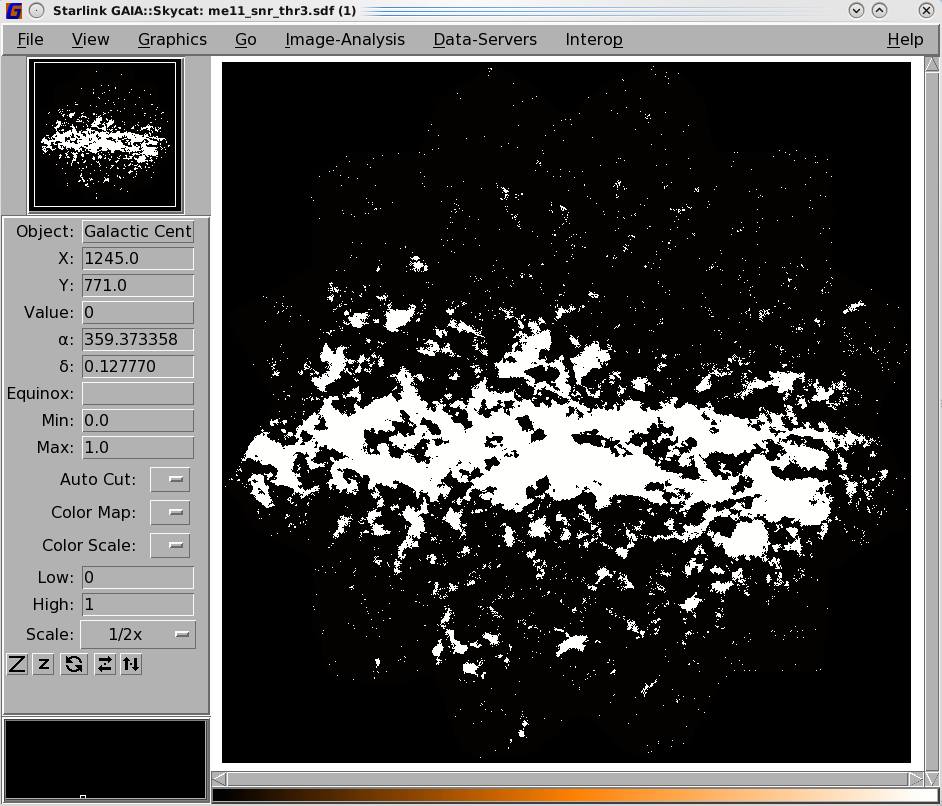
\includegraphics[width=0.475\linewidth]{sc21_gal_mask1}
\hspace{2mm}
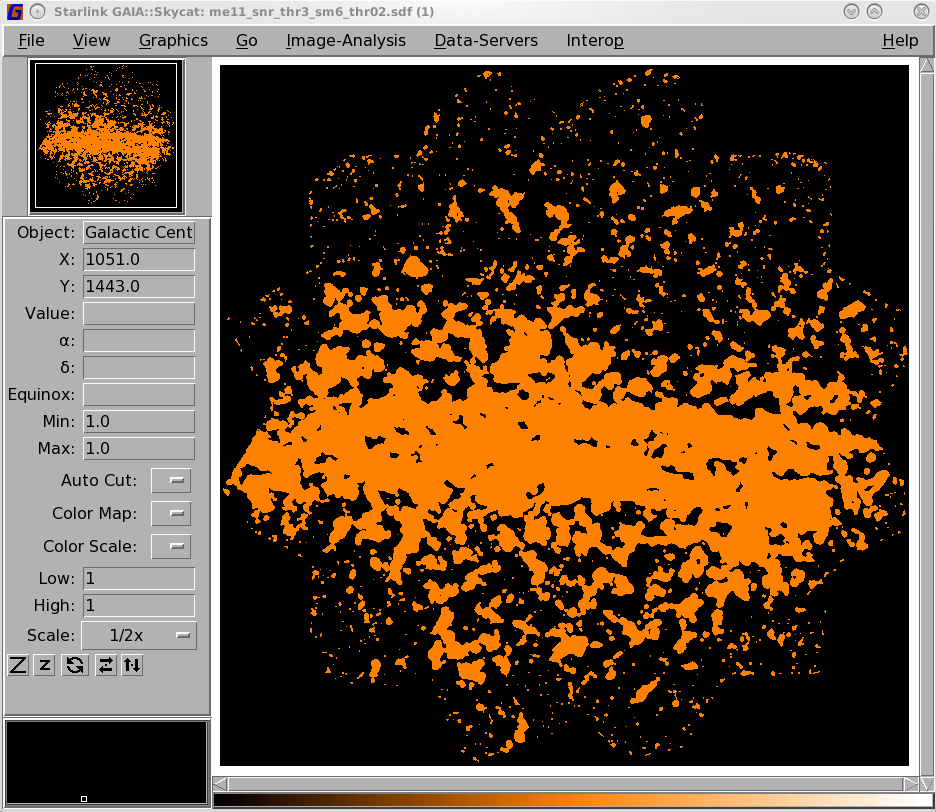
\includegraphics[width=0.475\linewidth]{sc21_gal_mask2}
\caption[Galactic example: thresholded SNR map and smoothed map]{
  \textbf{(Left)} The initial mask created by thresholding 850map\_snr
  to 3$\sigma$. \textbf{(Right)} Second mask made by thresholding the
  smoothed map to 0.02.\label{fig:mask}
}
\end{figure}


\textbf{Step 3: Re-running the map-maker with an external mask supplied}
\vspace{0.2cm}\\
As a last step the map is re-made with this mask supplied as an external
file. For this run we apply the additional parameters in a
personalised configuration file, \file{mydimmconfig.lis}.
\begin{terminalv}
% makemap in=^filelist.txt 850galactic method=iterate \
config=^mydimmconfig.lis ref=850map_mask_zm
\end{terminalv}

The configuration file, \file{mydimmconfig.lis}, has the following
format---note how it is based on
\file{dimmconfig\_bright\_extended.lis}. It has decreased the
convergence parameter to \param{MAPTOL}=0.03 but increased the number
of iterations to compensate as 40 is unlikely to be sufficient.
\begin{terminalv}
^$STARLINK_DIR/share/smurf/dimmconfig_bright_extended.lis
numiter = -100
noisecliphigh = 10.0
maptol = 0.03
ast.zero_mask=1
ast.zero_snr = 0
\end{terminalv}

\textbf{Step 4: Cropping the map}
\vspace{0.2cm}\\
We now crop the map to remove the noisy edges using the \picard\ recipe
\drrecipe{CROP\_JCMT\_IMAGES}. To determine what to trim we can look
at the exposure-time image with \gaia.  See
\cref{Figure}{fig:exptime}{the exposure time image}.

\starfig{sc21_gal_exptime}{[h!]}{width=0.7\linewidth}{fig:exptime}{
  Galactic example: exposure time map}{
  The exposure-time image of the science map from \cref{Figure}{fig:galmakemap}{
  our example map}. You can right-click and drag the mouse
  between two points to measure the distance. Here we see the exposure
  time dropping off sharply at a radius of 30\,arcmin. A non-default
  colour scale has been chosen to illustrate the morphology.
}

The exposure-time map shows a sharp drop off at a radius of 30\,arcmin.
We can thus specify a parameter file like below.
\begin{center}
\begin{terminalv}
[CROP_JCMT_IMAGES]
MAP_RADIUS = 1800
\end{terminalv}
\end{center}

\begin{terminalv}
% picard CROP_JCMT_IMAGES 850galactic.sdf
\end{terminalv}
The final cropped map is shown in \cref{Figure}{fig:crop_map}{this plot}.
Compared with the first map out of the map-maker
(\cref{Figure}{fig:galmakemap}{first map}),
slightly more of the faint extended emission is apparent.

One of the challenges facing this type of reduction is the need to
account for both faint extended structure and very bright sources in
the same map. You may find some degree of bowling remains around the
brightest sources.

There are areas you may wish to experiment with. One is to adjust the
filtering. Another option is to supply an external mask from
a different dataset, e.g. a
\htmladdnormallink{Herschel}{http://herschel.esac.esa.int/} map.
See \cref{Chapter}{sec:tweak}{Tailoring Your Reduction} for further
discussion.

\starfig{sc21_gal12_crop}{[b!]}{width=0.65\hsize}{fig:crop_map}{
  Galactic example: cropped final map}{
  The final cropped, reduced map from the map-maker run with
  an external mask supplied.
}


\clearpage
\chapter{\xlabel{pipeline}The SCUBA-2 Pipeline}
\label{sec:pipe}

\section{\xlabel{pl_overview}Pipeline overview}

SCUBA-2 data reduction pipelines have been developed based on the
existing \oracdr\ pipeline (Cavanagh et al., 2008\cite{oracdr}) used
for ACSIS. There are three distinct pipelines currently utilised by
SCUBA-2: two of these, the quick-look (QL) and summit pipelines, are
run in real time at the JCMT during data acquisition; the third, the science
pipeline, offers a comprehensive reduction, which users can run locally.

\begin{itemize}
\item The QL runs quality assurance checks on the data as it comes in.
For science data it calculates the noise between 2\,Hz and 10\,Hz,
along with the NEP and effective NEP, for each 30-second scan. These
values undergo quality-assurance checks to ensure SCUBA-2 is within
an acceptable operating range.
\item The summit pipeline is designed to provide a quick map of the
data, it does this by running fewer iterations and chunking the data
more. This is a useful guide to observers who wish to check the
quality of their data.
\item The science pipeline is run at CADC. This is normally the next
day once the data have transferred there.  This nightly processing
uses an optimal reduction routine, that includes the map-maker and a
number of post-processing steps (outlined below). Both the raw data
and reduced products are available for download by project members the
following day.
\end{itemize}

The manual for the SCUBA-2 pipeline can be found at \pipelinesun,
while the pipeline software comes as part of the \starlink\ suite.


\section{\xlabel{science_pl}The Science Pipeline}

The science pipeline will automate many of the steps discussed in
\cref{Chapter}{sec:maps}{Reducing Your Data}:
\vspace{-0.3cm}
\begin{itemize}\itemsep-0.3em
\item Run the iterative map-maker.
\item Apply the FCF to calibrate to mJy/beam.
\item Co-add multiple observations of the same object.
\item Apply the matched-filter (blank-field configuration file only)
\item Run a source-finding algorithm.
\end{itemize}

\subsection{\xlabel{pl_output}Pipeline recipes}
\label{sec:recipes}

When MSBs are created, the PI can select a pipeline recipe to assign
to the data. When the data are run through the science pipeline this
recipe is then called by default. This can overridden on the command
line---see \cref{Section}{sec:parameterfile}{Changing the defaults}.
Described below are the five main \oracdr\ science recipes.

\subsection{\xlabel{extsources}\drrecipe{REDUCE\_SCAN}}

\textbf{configuration file: \file{dimmconfig.lis}}

This recipe uses the default configuration file for \makemap, unless
the sources is identified as a calibrator. After all observations have
been processed the data are co-added and calibrated in mJy/beam using
the default FCF. The noise and NEFD properties for the co-add are
calculated and written to log files (\file{log.noise} and
\file{log.nefd} respectively). Finally, the \cupid\ task \findclumps\
is run using the FellWalker algorithm to create a source catalogue.

For calibrators, \file{dimmconfig\_bright\_compact.lis} is used and
FCFs are derived from the map.


\subsection{\xlabel{extsources}\drrecipe{REDUCE\_SCAN\_CHECKRMS}}

\textbf{Configuration file: \file{dimmconfig.lis}}

This recipe is the same as \drrecipe{REDUCE\_SCAN}, but includes extra
performance estimations determined by \drrecipe{SCUBA2\_CHECK\_RMS}
(see \cref{Section}{sec:checkrms}{Getting the noise}). These extra
metrics are written to a log file \file{log.checkrms}. Running
\drrecipe{SCUBA2\_CHECK\_RMS} in the pipeline, rather than as a
standalone \picard\ recipe, allows it to calculate results for
co-added maps.


\subsection{\xlabel{extsources}\drrecipe{REDUCE\_SCAN\_EXTENDED\_SOURCES}}

\textbf{Configuration file: \file{dimmconfig\_bright\_extended.lis}}

This is the recipe for processing extended sources. Multiple
observations are co-added and the output map is calibrated in units of
mJy/arcsec$^2$. This recipe also performs a source-finder routine; the
results are written as a FITS catalogue (with file extension
\file{.FIT}) which can be read as a local catalogue into \gaia.

\subsection{\xlabel{faint}\drrecipe{REDUCE\_SCAN\_FAINT\_POINT\_SOURCES}}

\textbf{Configuration file: \file{dimmconfig\_blank\_field.lis}}

This is the recipe for processing maps containing faint compact
sources. This time the configuration file called by \makemap\ is
\file{dimmconfig\_blank\_field.lis} and the map calibrated in
mJy/beam.  The output map is further processed with a matched filter,
then the S/N is taken to enhance point sources.  A map is written out
at each step.  This recipe also performs a source finder routine; the
results are written as a FITS catalogue (with file extension
\file{.FIT}) which can be read as a local catalogue into \gaia.


\subsection{\xlabel{faintjk}\drrecipe{FAINT\_POINT\_SOURCES\_JACKKNIFE}}

\textbf{Configuration file: \file{dimmconfig\_blank\_field.lis}}

This recipe uses a
\htmladdnormallink{jack-knife}{http://en.wikipedia.org/wiki/Jackknife_resampling}
method to remove residual low-spatial frequency noise and create an
optimal matched-filtered output map. The map-maker is run twice, first
as a standard reduction using \file{dimmconfig\_blank\_field.lis} (and
calibrated in mJy/beam), and the second time with a fake source added
to the time series. This creates a signal map and an effective PSF
map. A jack-knife map is generated from two halves of the dataset and
the maps are `whitened' by the removal of the residual 1/\emph{f}
noise. The whitened signal map is processed with the matched filter
using the whitened PSF map as the PSF input. The data are calibrated
in mJy/beam using a corrected FCF.  See \cref{Section}{sec:jk}{Example
  2 -- Advanced pipeline method} for a more-detailed description of
this recipe and the files produced.

\section{Changing the defaults}
\label{sec:parameterfile}
\subsection{Changing the pipeline recipe}
You can override the recipe set in the header by listing any different
one on the command line when starting \oracdr. For example
\begin{terminalv}
% oracdr -file mylist -loop file -log x REDUCE_SCAN_CHECKRMS
\end{terminalv}

You can find out which recipe is set in the data header via the FITS
header \texttt{RECIPE} keyword in any of your raw files.  For
example both of these options will return the same result:
\begin{terminalv}
% fitsval s8a20120725_00045_0003 RECIPE
% fitslist s8a20120725_00045_0003 | grep RECIPE
\end{terminalv}

\subsection{Changing the configuration file}

Although each recipe calls one of the standard configuration files
you can specify your own. You will need to create a recipe parameter
file. This file will set the parameter \param{MAKEMAP\_CONFIG} to be
your new configuration file. The first line must be the name of the
recipe used in the reduction.

For example, to run the pipeline with \drrecipe{REDUCE\_SCAN\_CHECKRMS} with a
configuration file called \file{myconfig.lis}, the recipe parameter file
(\file{mypars.ini}) will look like this.
\vspace{0.2cm}
\begin{terminalv}
[REDUCE_SCAN_CHECKRMS]
MAKEMAP_CONFIG = myconfig.lis
\end{terminalv}

Then run the pipeline calling the parameter file via the
\texttt{-recpars} option.
\begin{terminalv}
% oracdr -file mylist -loop file -log xf -recpars myparams.ini REDUCE_SCAN_CHECKRMS
\end{terminalv}


\section{\xlabel{running_pl}Running the Science Pipeline}
\label{sec:plsteps}


\begin{aligndesc}
\item[Step~1:]
\textbf{Initialise ORAC-DR}

This is done by:
\begin{terminalv}
% oracdr_scuba2_850 -cwd
\end{terminalv}

\item[Step 2:]
\textbf{Set environment variables}

These ensure the data are read from and written to the right
places. Many are set automatically when the pipeline is initialised
but others must be set manually. Details of the optional variables are
given in \pipelinesun\ but the three main ones are:

\begin{itemize}\itemsep-0.1em
\item \envvar{STARLINK\_DIR} -- Location of your Starlink installation.
\item \envvar{ORAC\_DATA\_IN} -- The location where the data should be read from.
If you are supplying a text file listing the raw data this should be the
location of that file.
\item \envvar{ORAC\_DATA\_OUT} -- The location where the data products should be
written. Also used as the location for a user-specified configuration file.
\end{itemize}

\item[Step 3:]
\textbf{(Optional) Create a personalised configuration file and/or parameter file}

See \cref{Section}{sec:parameterfile}{Changing the defaults} for
details. In this example we find the recipe \drrecipe{REDUCE\_SCAN}
assigned to our data. We are happy with the steps in this recipe but
want to supply a new configuration file and a different set of
clump-finding parameters. To do so we create a parameter file called
\file{mypars.ini} which contains the following text.

\begin{terminalv}
[REDUCE_SCAN]
MAKEMAP_CONFIG = mynewconfig.lis
FINDCLUMPS_CFG = myfellwalkerparams.lis

\end{terminalv}

\item[Step 4:]
\textbf{Run the pipeline}

Run the pipeline using the \texttt{-recpars} option to specify a
parameter file if required.
\begin{terminalv}
% oracdr -files inputlist.txt -loop file  -log xf -recpars mypars.ini
\end{terminalv}
\end{aligndesc}


\section{\xlabel{pl_output}Pipeline output}

The pipeline will produce a group file for each object being
processed. If the pipeline is given data from multiple nights, all
those data will be included in the group co-add using inverse variance
weighting.

The final maps in your output directory will have the suffix
\file{\_reduced}. Maps will be made for individual observations, which
will start with an \file{s} (e.g.
\file{s20140620\_00030\_850\_reduced.sdf}). Group maps, which may
contain co-added observations from a single night, are also produced
which have the prefix \file{gs}
(e.g. \file{gs20140620\_30\_850\_reduced.sdf}).

\textbf{Note:} A group file is \emph{always} created, even if only a
single observation is being processed.

Additionally, PNG images are made of the reduced files at a variety of
resolutions.

\section{\xlabel{cadc}Getting your data from CADC}

The JCMT Science Archive is hosted by The Canadian Astronomy Data
Centre (CADC). Both raw data and data processed by the science
pipeline are made available to PIs and co-Is through the CADC
interface (\url{http://www3.cadc-ccda.hia-iha.nrc-cnrc.gc.ca/jcmt/}).

To access proprietary data you will need to have your CADC username
registered by the JAC and thereby associated with the project code.

An important search option to be aware of is `Group Type', where your
options are Simple, Night, Project and Public. Simple (which becomes
`obs' on the result page) is an individual observation; night means
the group file from the pipeline (these may or may not include more
than one observation; the `Group Members' value will tell you); and
the project option is generated if an entire project has been run
through the pipeline and identical sources across the project are
co-added into master group files.


\begin{thebibliography}{}
\addcontentsline{toc}{section}{References}

\bibitem{archibald}
Archibald,~E.~N., et~al, 2002, \htmladdnormallink{\textit{On the atmospheric limitations
of ground-based submillimetre astronomy using array receivers}}{http://dx.doi.org/10.1046/j.1365-8711.2002.05582.x}, MNRAS, 336, 1-13
(DOI:10.1046/j.1365-8711.2002.05582.x)

\bibitem{oracdr}
Cavanagh~B., Jenness~T., Economou~F., Currie~M.~J., 2008,
\htmladdnormallink{\textit{The ORAC-DR data reduction
pipeline}}{http://dx.doi.org/10.1002/asna.200710944}, Astron. Nactr., 329, 295
(DOI:10.1002/asna.200710944)

\bibitem{smurf}
Chapin~E.~L., et~al., 2013, \textit{SMURF -- Sub-Millimetre User Reduction
Facility}, \xref{Starlink User Note 258}{sun258}{}

\bibitem{mapmaker}
Chapin~E.~L., et~al., 2013,
\htmladdnormallink{\textit{SCUBA-2: iterative map-making with the
Sub-Millimetre User Reduction Facility}}{http://dx.doi.org/10.1093/mnras/stt052},
MNRAS, 430, 2545 (DOI:10.1093/mnras/stt052)

\bibitem{ssds}
Currie~M.~J., Wallace~P.~T., Warren-Smith~R.~F., 1989,
\textit{Starlink Standard Data Structures}, \xref{Starlink General
Paper 38.2}{sgp38}{}

\bibitem{kappa}
Currie~M.~J., Berry~D.~S, 2013, \textit{KAPPA -- Kernel Application Package},
\xref{Starlink User Note 95}{sun95}{}

\bibitem{dempsey12}
Dempsey~J.~T. et al., 2013, \htmladdnormallink{\textit{SCUBA-2: on-sky calibration using
submillimetre standard sources}}{http://dx.doi.org/10.1093/mnras/stt090},
MNRAS, 430, 2534 (DOI:10.1093/mnras/stt090)

\bibitem{dempsey-spie}
Dempsey~J.~T., Friberg~P., Jenness~T., Bintley~D., Holland~W.~S., 2010
\htmladdnormallink{\textit{Extinction correction and on-sky calibration of
SCUBA-2}}{http://dx.doi.org/10.1117/12.856476},
Proc.\ SPIE, 7741 (DOI:10.1117/12.856476)

\bibitem{gaia}
Draper~P.~W., Gray~N., Berry~D.~S., Taylor~M., 2012,
\textit{GAIA -- Graphical Astronomy and Image Analysis Tool},
\xref{Starlink User Note 214}{sun214}{}

\bibitem{picard}
Gibb~A.~G., Jenness~T., Economou~F., 2012, \textit{PICARD --- a
PIpeline for Combining and Analyzing Reduced Data}
\xref{Starlink User Note 265}{sun265}{}

\bibitem{s2main}
Holland, W. S., et~al, 2013, \htmladdnormallink{\textit{SCUBA-2: The
10,000 pixel bolometer camera on the James Clerk Maxwell Telescope}}
{http://dx.doi.org/10.1093/mnras/sts612}, MNRAS, 430, 2513
(DOI:10.1093/mnras/sts612)

\bibitem{flux1}
Jenness~T., et~al, 2002, \htmladdnormallink{\textit{Towards the automated
reduction and calibration of SCUBA data from the James Clerk Maxwell
Telescope}}{http://dx.doi.org/10.1046/j.1365-8711.2002.05604.x},
MNRAS, 336, 14-21 (DOI:10.1046/j.1365-8711.2002.05604.x)

\bibitem{sc2ana005}
Scott~D., Van Engelen~A., 2005, \htmladdnormallink{\textit{Scan Mode Strategies for
SCUBA-2}}{http://docs.jach.hawaii.edu/JCMT/SC2/ANA/S210/005/sc2_ana_s210_005.ps},
SCUBA-2 Data Reduction document SC2/ANA/S210/005

\end{thebibliography}

\newpage
\appendix

\chapter{\xlabel{app_clean}Cleaning the raw data}
\label{app:clean}

You can use the \smurf\ task \clean\ to help inspect time-series.
\task{sc2clean} can be used to do two basic tasks in one go:
concatenate data (with or without applying a flatfield); and cleaning
(fix up steps and spikes, remove the means, filter, remove common-mode
etc.). It uses the same configuration files as the iterative map-maker
(though ignoring the map-making specific items).

In this first basic example, we just want to clean up some data enough
to see whether the bolometers have been flat-fielded correctly, and
more-or-less exhibit the same behaviour over time. The pre-processing
or cleaning steps used by the default configuration file are
summarised in \cref{Table}{tab:dimmdef}{this table}.

\begin{terminalv}
% sc2clean $FILES clean config=^$STARLINK_DIR/share/smurf/dimmconfig.lis
\end{terminalv}

Here \file{\$FILES} can just be a single file from a sub-array, or a
subset, e.g. \file{s8a20110417\_00051\_0003.sdf} (the first file
containing science data), \file{s8a20110417\_00051\_000"[1234]"} (File
1 is a noise observation with shutter closed that gets ignored, File 2
is a flatfield observation that will be used to override the flatfield
stored in the subsequent Files 3 and 4 which are concatenated
together, the \file{.sdf} is optional),
\file{s8a20110417\_00051\_000\textbackslash?} (Files 1 through 9),
\file{s8a20110417\_00051\_\textbackslash*} (the whole observation).

If you inspect the resulting \file{clean.sdf} in \gaia\
(\cref{Section}{sec:gaiacube}{Displaying time-series data}) and flip
through the data cube you should see all of the bolometers signals go
up and down together with about the same amplitude: the hope is that
for a well-behaved instrument you are mostly seeing sky noise
variations that are seen with roughly the same amplitude by all
bolometers.

Another common feature, if the scans are particularly long and/or fast
(e.g. 1\,degree across), is strong periodic signals that are
correlated with the scan pattern. See
\cref{Section}{sec:scan}{Displaying scan patterns}---in particular you
will want to plot \texttt{az} and \texttt{el} (the absolute azimuth
and elevation), and also \texttt{daz} and \texttt{del} (the azimuth
and elevation offsets from the map centre). This signal is usually
azimuth-correlated due to magnetic-field pickup. It only shows up in
azimuth, because the instrument is on a Nasmyth platform and therefore
does not move in elevation.

Part of the reason the signals look the same is because they have been
flatfielded. You can turn off flatfielding using the \param{noflat}
option to \task{sc2clean}, and you should then see that all of the
detector amplitudes vary.

Another very useful option is to remove the common signal observed by
all of the bolometers. This may be accomplished by

\begin{terminalv}
% sc2clean $FILES clean \
   config='"^$STARLINK_DIR/share/smurf/dimmconfig.lis,compreprocess=1"'
\end{terminalv}

The residual of this signal will exhibit second-order time-varying
correlated signals across the focal plane. Usually these are not very
large, but in some cases some very large localized signals have been
detected, particularly in the 850\,$\mu$m arrays in early 2011.

Another variation on this is to accentuate the residual low-frequency
noise by low-pass filtering the result. This can again be accomplished
by simply adding a filter command in the \param{config} parameter,
which in this case low-pass filters with a cutoff at 10\,Hz:

\begin{terminalv}
% sc2clean $FILES clean \
config='"^$STARLINK_DIR/share/smurf/dimmconfig.lis,compreprocess=1,filt_edgelow=10"'
\end{terminalv}

Finally, in some cases you might just want to fit and remove
polynomial baselines from the bolometers (by default only the mean is
removed). This example will remove a line, but you can increase the
value of \param{order} to remove higher-order polynomials

\begin{terminalv}
% sc2clean $FILES clean \
   config='"^$STARLINK_DIR/share/smurf/dimmconfig.lis,order=1"'
\end{terminalv}

Any of the cleaning parameter can be specified independently of the
default configuration files like so:
\begin{terminalv}
% sc2clean $FILES clean config='"order=1,dcfitbox=30,dcthresh=25,dcsmooth=50"'
\end{terminalv}
Or you can create your own customised configuration file. All the
pre-processing options that may be specified are listed and described
in \file{dimmconfig.lis}---see \cref{Appendix}{app:dimm}{here}.



\chapter{\xlabel{calib}SCUBA-2 data calibration}
\label{app:cal}

\section{\xlabel{fcf}Flux conversion factors (FCF)}
\label{app:fcf}

Primary and secondary calibrator observations have been reduced using
the specifically designed \file{dimmconfig\_bright\_compact.lis}.  The
maps produced from this are then analysed using tailor-made \picard\
recipes. For instructions on applying the FCFs to your map see
\cref{Section}{sec:cmult}{this page}.

A map reduced by the map-maker has units of pW. To calibrate the data
into units of janskys (Jy), a set of bright, point-source objects with
well-known flux densities are observed regularly to provide a flux
conversion factor (FCF). The data (in pW) can be multiplied by this
FCF to obtain a calibrated map. The FCF can also be used to assess the
relative performance of the instrument from night to night. The noise
equivalent flux density (NEFD) is a measure of the instrument
sensitivity, and while not discussed here, is also produced by the
\textsc{Picard} recipe shown here. For calibration of primary and
secondary calibrators, the FCFs and NEFDs have been calculated as
follows:

\begin{enumerate}
\item The \textsc{Picard} recipe \drrecipe{SCUBA2\_FCFNEFD} takes the
  reduced map, crops it, and runs background removal. Surface-fitting
  parameters are changeable in the \textsc{Picard} parameter file.

\item It then runs the \Kappa\ \beamfit\ task on the specified point
  source. The \task{beamfit} task will estimate the peak
  (uncalibrated) flux density and the FWHM. The integrated flux
  density within a given aperture (30-arcsec radius default) is
  calculated using \photom\ \autophotom. Flux densities for
  calibrators such as Uranus, Mars, CRL~618, CRL~2688 and HL~Tau are
  already known to \picard. To derive an FCF for other sources of
  known flux densities, the fluxes can be added to the parameter file
  with the source name (in upper case, spaces
  removed): \param{FLUX\_450.MYSRC~=~0.050}
  and \param{FLUX\_850.MYSRC~=~0.005} (where the values are in Jy),
  for example.

\item Three different FCF values are calculated, two of which are
  described below.

  \begin{enumerate}

  \item \textbf{The arcsecond FCF}
    \begin{equation}
      \label{eq:fcf_arcsec}
      \mathrm{FCF_{arcsec}} = \frac{S_{\mathrm{tot}}}{P_{\mathrm{int}} \times
        A_{\mathrm{pix}}}
    \end{equation}

    where $S_{\mathrm{tot}}$ is the total flux density of the
    calibrator, $P_{\mathrm{int}}$ is the integrated sum of the source
    in the map (in pW) and $A_{\mathrm{pix}}$ is the pixel area in
    arcsec$^2$, producing an FCF in Jy/arcsec$^2$/pW.

  \item\textbf{The beam FCF}
    \begin{equation}
      \label{eq:fcf_beam}
      \mathrm{FCF_{beam}} = \frac{S_{\mathrm{peak}}}{P_{\mathrm{peak}}}
    \end{equation}
    producing an FCF in units of Jy/beam/pW.
  \end{enumerate}

\end{enumerate}

The measured peak signal here is derived from the Gaussian fit of
\task{beamfit}. The peak value is susceptible to pointing and focus
errors, and we have found this number to be somewhat unreliable,
particularly at 450$\mu$m.


\section{\xlabel{extinction}Extinction correction}

Analysis of the SCUBA-2 secondary calibrators has allowed calculation
of the transmission relationships for the SCUBA-2 450\,$\mu$m and
850\,$\mu$m pass-bands to be determined. Full details of the analysis
and on-sky calibration methods of SCUBA-2 can be found in Dempsey et
al.\ (2013)~\cite{dempsey12}\cite{dempsey-spie}.

Archibald et al. (2002)\,\cite{archibald} describes how the Caltech
Submillimeter Observatory (CSO) 225\,GHz opacity, $\tau_{225}$,
relates to SCUBA opacity terms in each band, $\tau_{450}$ and
$\tau_{850}$. The JCMT water-vapour radiometer (WVM) uses the 183\,GHz
water line to calculate the precipitable water vapour (PWV) along the
line-of-sight of the telescope. This PWV is then input into an
atmospheric model to calculate the zenith opacity at 225\,GHz
($\tau_{225}$). This allows ease of comparison with the adjacent CSO
225\,GHz tipping radiometer. The opacities have been as:

\begin{equation}
\tau_{450} = 26.0 \times (\tau_{225} - 0.012);
\end{equation}
and
\begin{equation}
\tau_{850} = 4.6 \times (\tau_{225} - 0.0043).
\end{equation}

The SCUBA-2 filter characteristics are described in detail
\htmladdnormallinkfoot{on the JCMT
  website}{http://www.jach.hawaii.edu/JCMT/continuum/scuba2/filter/}.

The extinction correction parameters that scale from $\tau_{225}$ to
the relevant filter have been added to the map-maker code. You can
override these values by setting \param{ext.taurelation.filtname} in
your map-maker config files to the two coefficients `($a$,$b$)' that
you want to use (where \param{filtname} is the name of the
filter). The defaults are listed in
\file{\$SMURF\_DIR/smurf\_extinction.def}.

% It is worth noting that if an individual science map and
% corresponding calibrator observation has already been reduced with
% the old factors (and your source and calibrator are at about the
% same airmass and if the tau did not change appreciably), any errors
% in extinction correction should cancel out in the calibration.

\chapter{\xlabel{calcrms}\drrecipe{SCUBA2\_CHECK\_RMS}}
\label{app:checkrmsparams}

The \picard\ recipe \drrecipe{SCUBA2\_CHECK\_RMS} estimates the RMS
and NEFD for a given observation via two methods to compare with
values from the SCUBA-2 integration time calculator (ITC).

The average NEP is calculated from the QL pipeline log file
(\file{log.nep}) corresponding to the date and wavelength. The FCF
(either from the file or the standard value) and mean transmission
over the observation is used to convert this to a zenith NEFD
(NEFD\_NEP). The elapsed time is used to convert that to an RMS noise
(RMS\_NEP).

The input images are cropped to the given size (as specified in the
FITS headers or via the MAP\_HEIGHT and MAP\_WIDTH recipe parameters)
before the mean exposure time is derived, along with the mean/median
noise and NEFD (RMS\_MAP and NEFD\_MAP).

The RMS corresponding to the observation type is calculated from the
SCUBA-2 ITC (RMS\_ITC); the time is used to convert that to a
corresponding NEFD (NEFD\_ITC).

The parameters written out to \file{log.checkrms} are listed below:
\begin{table}[h!]
  \begin{center}
    \begin{tabular}{|p{2.5cm}|p{12cm}|}
      \hline
      \textbf{Parameter} & \textbf{Description}\\
      \hline
      UT & UT date including day fraction\\
      Source & object name, upper case with spaces removed\\
      Obs & observation number\\
      FILTER & filter (wavelength)\\
      telapsed & elapsed time of observation in seconds\\
      texp & mean exposure time, derived from EXP\_TIME NDF component (sec)\\
      trans & mean line-of-sight transmission\\
      nep\_av & mean NEP for current observation (W/sqrt(Hz))\\
      nep\_av\_err & uncertainty in nep\_av (W/sqrt(Hz))\\
      rms\_nep & RMS derived from nefd\_nep (mJy/beam)\\
      nefd\_nep & NEFD derived from nep\_av and scaled elapsed time (mJy sqrt(sec))\\
      rms\_map & RMS noise in map, obtained from median of error array (mJy/beam)\\
      nefd\_map & NEFD derived from combination of variance and exposure time images (mJy sqrt(sec))\\
      rms\_itc & RMS noise estimated by SCUBA-2 integration time calculator (ITC) (mJy/beam) \\
      nefd\_itc & NEFD derived from rms\_itc and scaled elapsed time (mJy sqrt(sec)) \\
      itc\_obstype & observation type used by the ITC to derived RMS\\
      rms\_ratio & ratio of rms\_map to rms\_itc\\
      El & mean elevation in degrees\\
      CSO & mean zenith optical depth at 225 GHz, derived from WVM\\
      Tau & mean zenith optical depth at the current wavelength (given by FILTER above)\\
      Radius & radius in arcsec of image used in analysis\\
      pixscale & pixel scale in arcsec\\
      f & ITC f parameter\\
      project & project ID\\
      \hline
    \end{tabular}
  \end{center}
\end{table}


\chapter{\xlabel{matchedfilter}SCUBA-2 matched filter}
\label{app:mf}

In order to optimally find sources that are the size of the telescope
beam, and suppress this residual large-scale noise, the \picard\
recipe \drrecipe{SCUBA2\_MATCHED\_FILTER} may be used. If there were
no large-scale noise in the map, the filtered signal map would be
calculated as follows:

\begin{equation}
  {\cal{M}} = \frac{[M(x,y)/\sigma^2(x,y)] \otimes P(x,y)}
  {[1/\sigma^2(x,y)] \otimes [P^2(x,y)]},
\end{equation}

where $M(x,y)$ and $\sigma(x,y)$ are the signal and RMS noise maps
respectively produced by \smurf, and $P(x,y)$ is a map of the
PSF. Here \(\otimes\)
denotes the 2-dimensional cross-correlation operator. Similarly, the
variance map would be calculated as

\begin{equation}
  {\cal{N}}^2 = \frac{1}{[1/\sigma^2(x,y)] \otimes [P^2(x,y)]}.
\end{equation}

This operation is equivalent to calculating the maximum-likelihood fit
of the PSF centered over every pixel in the map, taking into account
the noise. Presently $P(x,y)$ is simply modelled as an ideal Gaussian
with a FWHM set to the diffraction limit of the telescope.

However, since there is large-scale (and therefore correlated from
pixel to pixel) noise, the recipe also has an additional step. It
first smooths the map by cross-correlating with a larger Gaussian
kernel to estimate the background, and then subtracts it from the
image. The same operation is also applied to the PSF to estimate the
effective shape of a point-source in this background-subtracted map.

Before running \textsc{Picard}, a simple parameters file called
\file{smooth.ini} may be created.
\begin{terminalv}
[SCUBA2_MATCHED_FILTER]
SMOOTH_FWHM = 15
\end{terminalv}
%
where \param{SMOOTH\_FWHM~=~15} indicates that the background should
be estimated by first smoothing the map and PSF with a 15~arcsec FWHM
Gaussian. The recipe is then executed as follows:
%
\begin{terminalv}
% picard -recpars smooth.ini SCUBA2_MATCHED_FILTER map.sdf
\end{terminalv}
%
The output of this operation is a smoothed image called
\file{map\_mf.sdf}. By default, the recipe automatically normalizes
the output such that the peak flux densities of point sources are
conserved. Note that the accuracy of this normalization depends on how
closely the real PSF matches the 7.5~arcsec and 14~arcsec full-width
at half-maximum (FWHM) Gaussian shapes assumed at 450$\mu$m and
850$\mu$m, respectively (an explicit PSF can also be supplied using
the \param{PSF\_MATCHFILTER} recipe parameter).


\chapter{\xlabel{fcfsred}FCFs by reduction date}
\label{app:fcfs}

Ongoing development of the SCUBA-2 analysis has resulted in ongoing
changes to the tau relationship and the FCFs. Depending on when your
data were reduced you will need to apply different calibration values.
\\
\begin{table}[h!]
\begin{center}
\begin{tabular}{|l|c|c|c|c|}
 \hline
 \multicolumn{1}{|c|}{Date} &
 \multicolumn{2}{c|}{FCF - 450$\mu$m} &
 \multicolumn{2}{c|}{FCF - 850$\mu$m} \\
\cline{2-5}
& Jy/pW/beam &Jy/pW/arcsec$^2$ & Jy/pW/beam &Jy/pW/arcsec$^2$ \\
 \hline
until January 2012 &383  & 4.9&1080 &5.0 \\
January 2012 - July 2012&606&6.06 &556 &2.42 \\
July 2012 onwards&491 &4.71 &537 &2.34 \\
\hline
\end{tabular}
\end{center}
\end{table}
\vspace{-2mm}
\begin{table}[h!]
\begin{center}
\begin{tabular}{|l|c|c|}
 \hline
 \multicolumn{1}{|c}{Date} & \multicolumn{2}{|c|}{Tau Relation}  \\ \cline{2-3}
                           & 450$\mu$m  & 850$\mu$m \\ \hline
until January 2012       & 32 $\times$ ($\tau_{225}$ - 0.02)    & 5.2 $\times$ ($\tau_{225}$ - 0.013)  \\
January 2012 - July 2012 & 26 $\times$ ($\tau_{225}$- 0.01923)  & 4.6 $\times$ ($\tau_{225}$ - 0.00435)  \\
July 2012 onwards        & 26 $\times$ ($\tau_{225}$ - 0.01196) & 4.6 $\times$ ($\tau_{225}$ - 0.00435)  \\
\hline
\end{tabular}
\end{center}
\end{table}

\vspace{-5mm}
\begin{itemize}
\item Peak FCF (Jy/pW/beam)---multiply your map by this when you wish
to measure absolute peak fluxes of discrete sources.
\item Arcsec FCF (Jy/pW/arcsec$^2$)---multiply your map by this if
you wish to use the calibrated map to do aperture photometry.
\end{itemize}
You can find out when your data was reduced and hence what tau
relation was applied by using the \Kappa\ command \hislist.
\vspace{-2mm}
\begin{terminalv}
%  hislist file | grep EXT.TAURELATION
\end{terminalv}
This will return something like the following,
\begin{terminalv}
      EXT.TAURELATION.450=(26.0,-0.012),
      EXT.TAURELATION.850=(4.6,-0.0043), EXT.TAUSRC=auto, FAKESCALE=1,
\end{terminalv}

\newpage
\chapter{\xlabel{cog}Aperture-photometry curve of growth}
\label{app:cog}

The SCUBA-2 beam has a broad error beam. As the size of the annulus
changes, the contribution from the error beam scales according to the
curve-of-growth---see \cref{Figure}{fig:cog}{the figure below}. To correct for an
aperture size differing from 60-arcsec diameter you should read off the
appropriate scaling factor for your FCF from the graph below.

\starfig{sc21_curveofgrowth}{[h!]}{width=\linewidth}{fig:cog}{
  Aperture photometry curve of growth}{
  Aperture photometry curve of growth normalised for a 60-arcsec
  aperture at 450$\mu$m \textbf{(left)} and 850$\mu$m
  \textbf{(right)}. Figure taken from Dempsey et al. (2013).
}

\newpage
\chapter{\xlabel{fits}Convert format from FITS to NDF}
\label{app:fits}

It is often useful to utilise data from other wavelengths or
instruments (either for a comparison or for an external mask). In the
following example, the FITS file called \file{file.fits} is
converted to NDF format as \file{file.sdf} using the \starlink\
package \convert. Note that the \file{.sdf} file extension NDF may
be omitted to save typing.

\begin{terminalv}
% convert
% fits2ndf file.fits file.sdf
\end{terminalv}

Unless your FITS file is from a recognised source, \fitstondf\ puts the
various FITS extensions into NDF extensions called FITS\_EXT\_$<n>$,
where $n$ counts from one for the first FITS extension. These are
located in the top-level MORE component of the NDF. If one of these is
the array you want---it should be an NDF too---it will be easier to
handle if you copy out of the NDF extension to its own NDF.

\begin{terminalv}
% ndfcopy in=file.more.fits_ext_1 out=file_data
\end{terminalv}

If there is a variance array stored in another extension that you want
to attach to your new NDF, a command like the following will do that.

\begin{terminalv}
% setvar ndf=file_data from=file.more.fits_ext_2
\end{terminalv}

\task{fits2ndf} does offer a way of mapping FITS extensions to familiar NDF
array components DATA, VARIANCE, and QUALITY through the \param{EXTABLE} file,
avoiding the \ndfcopy\ and possible \setvar\ steps.


\newpage
\chapter{\xlabel{defconfig}Default dimmconfig.lis}
\label{app:dimm}
\raggedbottom


\begin{sllongtable}{|l|p{1.0cm}|p{11.2cm}|}{%
\label{tab:dimmdef} The variables listed in \file{dimmconfig.lis} and
their default values. For a fuller description of each, as well as
other options, see the comments in \file{smurf\_makemap.def}, or the
\textit{Configuration Parameters} appendix of \textbf{SUN/258}.}
\hline
Parameter & Value & Description \\ \hline
\endhead

\hline
\endfoot

\multicolumn{3}{|l|}{\textbf{General}}\\
\hline
\param{numiter}       & $-$5 & Number of iterations, where a negative number
                               is the maximum number of iterations
                               if using $\chi^2$ and/or map-stopping criteria \\
\param{maptol}        & 0.05 & Threshold change in the map between consecutive
                               iterations \\
\param{chitol}        & undef& Alternative convergence criterion \\
\param{varmapmethod}  &    1 & Estimate variance map by sample variance of data that
                               land in each pixel \\

\param{exportndf}     &    0 & Do not export any models \\
\param{itermap}       &    0 & Do not export itermaps \\
\param{bolomap}       &    0 & Do not export bolometer maps \\
\param{shortmap}      &    0 & Do not export short maps \\

\hline
\multicolumn{3}{|l|}{\textbf{Pre-processing}}\\
\hline
\param{downsampscale} & $-$1 & Down-sample to save memory and time, where a negative
                               value's magnitude will be multiplied by the
                               \param{pixsize} for the requested map \\
\param{maxlen}        &    0 & Maximum length (secs) for concatenated data, where
                               0 requests concatenation of entire chunks \\
\param{order}         &    1 & Subtract a baseline polynomial of this order \\
\param{doclean}       &    1 & Allows pre-cleaned data to be used \\
\param{exportclean}   &    0 & Do not export clean model \\
\param{badfrac}       & 0.05 & Fraction of samples to be bad to flag entire bolometer
                               as dead \\
\param{flagslow}      &   30 & Flag data taken while telescope was moving so slowly
                               that sources sit in $1/f$ noise \\
\param{flagfast}      & 1000 & Flag data taken the telescope was moving too fast
                               causing source smearing \\
\param{filt\_edgelow} &    0 & Specifies the highest frequency to be retained by the
                               initial data cleaning \\
\param{spikethresh}   &    0 & The S/N at which to flag spikes during the initial
                               data cleaning \\
\param{spikebox}      &   50 & Size of the filter box for the sigma-clipper used for
                               spike detection in the initial data cleaning \\
\param{pcathresh}     &    0 & PCA cleaning is the threshold above which components
                               will be removed from the bolometer time-series \\
\param{pcalen}        &    0 & This specifies the chunk length that will be cleaned
                               as a number of time slices \\
\param{dcthresh}      & 25.0 & S/N threshold to detect DC step \\
\param{dcfitbox}      &   30 & Box size over which to fit data with a straight
                               line on either side of a potential DC jump \\
\param{dcmaxsteps}    &   10 & The maximum number of steps that can be corrected
                               in each minute of good data \\
\param{dclimcorr}     &    0 & If more than \param{dclimcorr} bolometers have a step
                               at a given time, then all bolometers are corrected
                               for a step at that time, using lower thresholds \\
\hline

\hline
Parameter & Value & Description \\
\hline
\multicolumn{3}{|l|}{\textbf{Pre-processing (continued)}}\\
\hline
\param{dcsmooth}      &   50 & The width of the median filter used to smooth a
                               bolometer data stream prior to finding DC jump \\
\param{noisecliphigh} &  4.0 & Clip bolometers based on their noise. This step
                               will remove any bolometers noisier than
                               \param{noisecliphigh}
                               standard deviations above the median \\
\param{noisecliplow}   &   0 & Do not clip any bolometers with low noise \\
\param{noisecliprecom} &   0 & This sets the noise clipping to occur prior to
                               \model{COM} subtraction instead of at the end of
                               the cleaning phase \\
\param{whiten}         &   0 & If non-zero a whitening filter is applied to each
                               time stream prior to any filtering in the
                               data-cleaning stage \\
\param{compreprocess}  &   0 & If non-zero, the \model{COM} is removed before the
                               iterative algorithm begins \\
\hline
\multicolumn{3}{|l|}{\textbf{Pre-process: fakemaps}}\\
\hline
\param{fakemap}        & undef & Diagnostic tool to explore the effects of the
                                 map-making process on known sources \\
\param{fakescale}      &     1 & Control the use of the supplied fake map \\
\hline
\multicolumn{3}{|l|}{\textbf{Iterative}}\\
\hline
\param{com.perarray}     &      0 & If non-zero, calculate a separate common-mode
                                    signal for each sub-array \\
\param{com.niter}        &      1 & The number of $n$-sigma clipping iterations
                                    (1 = no clipping) \\
\param{com.nsigma}       &      3 & The number of standard deviations at which the
                                    $\sigma$-clipping algorithm trims \\
\param{com.noflag}       &      0 & If set, disable flagging of bad bolometers
                                    using common-mode \\
\param{com.corr\_tol}    &      5 & Number of sigma away from mean
                                    correlation-coefficient tolerance \\
\param{com.corr\_abstol} &      5 & Number of sigma away from mean
                                    correlation-coefficient tolerance \\
\param{com.gain\_tol}    &      5 & Number of sigma away from mean gain-coefficient
                                    tolerance \\
\param{com.gain\_abstol} &      3 & Absolute factor away from mean gain-coefficient
                                    tolerance \\
\param{com.gain\_box}    &$-$30.0 & The number of time slices (or seconds if
                                    negative) in a box \\
\param{com.gain\_fgood}  &   0.25 & The minimum fraction of good gain boxes for a
                                    usable bolometer \\
\param{com.gain\_rat}    &      4 & The ratio of the largest usable gain to the
                                    mean gain for a bolometer not to be rejected \\
\param{com.zero\_mask}   &      0 & Whether or not to use \model{COM} masking \\
\param{com.zero\_circle} &  undef & Defines the mask as a circle with a specified
                                    radius \\
\param{com.zero\_lowhits}&      0 & Excludes pixels that contain too few data
                                    samples from the mask \\
\param{com.zero\_snr}    &      0 & Excludes samples from the \model{COM} estimate
                                    that fall within map pixels with S/N values
                                    greater than \param{com.zero\_snr} \\
\param{com.zero\_snrlo}  &      0 & The basic mask created by thresholding at
                                    the S/N value specified by
                                    \param{com.zero\_snr} is allowed
                                    to expand down to an S/N equal to
                                    \param{com.zero\_snrlo} \\
\param{com.zero\_union}  &      1 & Defines how multiple \model{COM} masks
                                    are combined \\
\param{com.zero\_freeze} &      0 & Freezes the \model{COM} model after
                                    \param{com.zero\_freeze} iterations \\

\hline
\param{noi.calcfirst}    &      0 & If a non-zero value is supplied, the bolometer
                                    noise levels are calculated immediately after
                                    pre-conditioning \\
\param{noi.box\_size}    &      0 & Specifies the number of time slices used to
                                    determine the noise level in a section of a
                                    bolometer time stream \\
\hline
\hline
Parameter & Value & Description \\
\hline
\multicolumn{3}{|l|}{\textbf{Iterative (continued)}}\\
\hline
\param{flt.notfirst}     &      0 & If non-zero then low frequencies will not be
                                    removed from the time streams on the first
                                   iteration \\
\param{450.flt.filt\_-} & \multirow{2}{*}{600} &
                                   \multirow{4}{*}{{\Huge$\rbrace$}
                                   \begin{minipage}{9.8cm}Apply a frequency filter
                                   to the \model{FLT} model. The value is given in
                                   arcsecs which the map-maker converts to
                                   frequency.\end{minipage} } \\
\param{edge\_largescale}     &        & \\
\param{850.flt.filt\_-} & \multirow{2}{*}{300} & \\
\param{edge\_largescale}     &        & \\

\param{flt.zero\_mask}   &      0 & Whether or not to use \model{FLT} masking \\
\param{flt.zero\_circle} &  undef & Defines the mask as a circle with a specified
                                   radius \\
\param{flt.zero\_lohits} &      0 & Excludes pixels that contain too few data samples
                                   from the mask \\
\param{flt.zero\_snr}    &      0 & Excludes samples from the \model{FLT} estimate
                                    that fall within map pixels with S/N values
                                    greater than \param{flt.zero\_snr} \\
\param{flt.zero\_snrlo}  &      0 & The basic mask created by thresholding at the
                                    S/N value specified by
                                    \param{flt.zero\_snr} is allowed to expand
                                    down to an S/N equal to
                                    \param{flt.zero\_snrlo} \\
\param{flt.zero\_niter}  &      2 & The number of iterations for which the
                                    \model{FLT} model should be masked \\
\param{flt.zero\_union}  &      1 & Defines how multiple \model{FLT} masks are
                                    combined \\
\param{flt.zero\_freeze} &      0 & Freezes the \model{FLT} model after
                                    \param{com.zero\_freeze} iterations \\
\param{ext.tausrc}       &   auto & Options = auto, wvmraw, csotau, filtertau \\
\param{ext.taumethod}    &adaptive& Options = adaptive, full, quick \\
\param{ext.csotau}       &  undef & Specifies the CSO tau value to be used by the
                                    \model{EXT} model \\
\param{ext.filtertau}    &  undef & Used if parameter \param{ext.tausrc} is set
                                    to \param{filtertau} \\

\hline
\param{ast.mapspike}     &     10 & Throw away spikes in the \model{AST} map greater
                                    than $n$-$\sigma$, excluding the first iteration \\
\param{ast.zero\_mask}   &      0 & Whether or not to use \model{AST} masking \\
\param{ast.zero\_circle} &  undef & Defines the mask as a circle with a specified
                                    radius \\
\param{ast.zero\_lohits} &      0 & Excludes pixels that contain too few data
                                    samples from the mask \\
\param{ast.zero\_snr}    &      0 & Excludes samples from the \model{AST} estimate
                                    that fall within map pixels with S/N values
                                    greater than \param{ast.zero\_snr} \\
\param{ast.zero\_snrlo}  &      0 & The basic mask created by thresholding at the
                                    S/N specified by
                                    \param{ast.zero\_snr} is allowed to expand down
                                    to an S/N equal to \param{ast.zero\_snrlo} \\
\param{ast.zero\_snr\_fwhm} &   0 & The map-maker produces two maps. The first is
                                    created normally using the mask specified by
                                    \param{ast.zero\_snr.} The final S/N-based mask
                                    is smoothed using a Gaussian with FWHM equal to
                                    \param{ast.zero\_snr\_fwhm} (in arcsec). The
                                    map-maker is re-run using this smoothed mask
                                    to create the final map \\
\param{ast.zero\_snr\_low} &$-$1.1& Sets the value (0.0 to 1.0) at which to
                                    threshold the smoothed mask specified by
                                    \param{ast.zero\_snr\_fwhm} \\
\param{ast.zero\_union}  &      1 & Defines how multiple \model{AST} masks are
                                    combined \\
\param{ast.zero\_freeze}  &     0 & Freezes the \model{AST} model after
                                    \param{com.zero\_freeze} iterations \\
\hline

\end{sllongtable}




\chapter{\xlabel{special}Specialised configuration files}
\label{app:special}

\section{\file{dimmconfig\_bright\_extended.lis}}
\begin{terminalv}
^$STARLINK_DIR/share/smurf/dimmconfig.lis
   numiter=-40
   flt.filt_edge_largescale=480
   ast.zero_snr=3
   ast.zero_snrlo=2

   ast.skip=5
   flt.zero_snr=5
   flt.zero_snrlo=3

\end{terminalv}

\section{\file{dimmconfig\_bright\_compact.lis}}
\begin{terminalv}

^$STARLINK_DIR/share/smurf/dimmconfig_bright.lis
   numiter=-40

#  Per array common-mode should be fine here since we are dealing with
#  a compact source. It seems to make things more stable.
   com.perarray = 1

#  We can get away with harsher filtering since the boundary conditions are
#  quite tight
   flt.filt_edge_largescale=200

#  Use boundary constraints since the source is assumed to be isolated
   ast.zero_circle = (0.0166666666)

#  Mask the data when forming th FLT model in order to exclude the
#  source. This only happends on the first two iterations. This usually
#  speeds up convergence.
   flt.zero_circle = (0.0166666666)

\end{terminalv}


\section{\file{dimmconfig\_blank\_field.lis}}
\begin{terminalv}
   ^$STARLINK_DIR/share/smurf/dimmconfig.lis

   numiter = 4

#  No FLT model is needed since we are filtering out low frequencies as
#  part of the initial cleaning process.
   modelorder = (com,ext,ast,noi)

#  Use time-domain de-spiker first because we are only doing a single
#  FFT-based high-pass filter before the iterations start.
   spikethresh = 10

#  Heavier high-pass filtering. Note that the default padding/apodization
#  that will be used is the number of samples that corresponds to the
#  period of the knee frequency in the high-pass filter (i.e. 200*(1/freq) )
   filt_edge_largescale = 200

#  Large-scale structure is not an issue so treat each sub-array
#  independently for common-mode removal
   com.perarray = 1

\end{terminalv}



\section{\file{dimmconfig\_bright.lis}}

This file is included as although it is not used in its own right it
form the basis (on top of \file{dimmconfig.lis} for both
\file{dimmconfig\_bright\_compact.lis} and
\file{dimmconfig\_bright\_extended.lis}
\begin{terminalv}

   ^$STARLINK_DIR/share/smurf/dimmconfig.lis

   numiter = 20

#  Much weaker bolometer noise clip
   noisecliphigh = 10.0

#  Less aggressive DC step finder to avoid problems with bright sources
   dcthresh = 100

#  Less aggressive bolo flagging.
   com.corr_tol = 7
   com.gain_tol = 7
   com.gain_abstol = 5
\end{terminalv}

\newpage
\chapter{Configuration-parameter descriptions}
\label{app:parameters}
\chapter{\xlabel{selpars}Configuration-parameter Descriptions}
\label{app:parameters}

This appendix describes some of the \makemap\ configuration parameters
that are more likely to be of interest to a typical user. Thus parameters
relating to experimental or deprecated features, or features that should
not normally need to be changed, are not included here. For a complete list
of all available configturation parameters, see
\xref{SUN/258}{sun258}{par_full}.

\begin{itemize}
\item The ``SMURF Usage'' section of each description lists the \SMURF commands
that accept the parameter. This does not mean that all the
listed commands actually \emph{use} the parameter---it just means that
any commands \emph{not} in the list will report an error if the parameter
is supplied.
\item The default value for each parameter is shown in square brackets at
the end of the description. These default values are defined in the file
\texttt{\$SMURF\_DIR/smurf\_makemap.def} and are the values that are used
for any parameters that are not assigned a value within the configuration
file supplied to \makemap. In other words, any parameter values supplied
within a configuration file will be used instead of these default values.
\end{itemize}
\ifpdf
\else
~\newline
\textbf{\large Alphabetical listing:} \newline
See \cref{Appendix}{app:catpars}{Configuration parameters listed by
category} for classified listings.
\fi

\sstminitoc{}
\sstnomaintoc
% This file was created using:
%
%	applications/smurf/defaults/make_pardocs \
%		selected_params.lis \
%		selected_params.tex \
%		../../../applications/smurf/defaults 
%


\section{General Iterative }
\sstminitoc{}


\sstroutine{
   NUMITER
}{
   Determines when to stop iterating
}{
   \sstdescription{
      If a positive number is supplied, the specified number of
      iterations will always be performed. If a negative number is
      supplied, the absolute value gives the maximum number of
      iterations to perform. Fewer iterations will be performed if
      the termination criteria specified by parameter {\tt{"}}\xref{maptol}{sun258}{MAPTOL}{\tt{"}} and
      parameter {\tt{"}}\xref{chitol}{sun258}{CHITOL}{\tt{"}} are both met before {\tt{"}}-numiter{\tt{"}}
      iterations have been performed. [-5]
   }
   \sstattributetype{
      real
   }
   \sstdiytopic{
      SMURF Usage
   }{
      MAKEMAP, CALCQU
   }
}

\sstroutine{
   MAPTOL
}{
   Specifies when to stop iterating
}{
   \sstdescription{
      If the normalised change (either the mean or maximum change -
      see parameter {\tt{"}}\xref{maptol\_mean}{sun258}{MAPTOL_MEAN}{\tt{"}}) between the maps created on
      subsequent iterations falls below the value of maptol, then the
      map-maker performs one more iteration and then terminates. Only
      used if parameter {\tt{"}}\xref{numiter}{sun258}{NUMITER}{\tt{"}} is negative. The normalised mean
      (or maximum) change between maps is defined as the mean (or
      maximum) of the absolute change in map pixel value, taken
      over all pixels within the region of the AST mask (if any,
      see parameter {\tt{"}}\xref{ast.zero\_mask}{sun258}{AST.ZERO_MASK}{\tt{"}}, etc), and normalised by the RMS
      of the square root of the pixel variances. Compared to parameter
      {\tt{"}}\xref{chitol}{sun258}{CHITOL}{\tt{"}}, this is much more like a {\tt{"}}by eye{\tt{"}} test, that will stop
      the solution when the map stops changing. [0.05]
   }
   \sstattributetype{
      real
   }
   \sstdiytopic{
      SMURF Usage
   }{
      MAKEMAP, CALCQU
   }
}


\sstroutine{
   MODELORDER
}{
   Determines which models to include in the iterative
   process, and the order in which they are evaluated
}{
   \sstdescription{
      This should be a comma-separated list, in parentheses,
      containing one or more of the following model names, in the
      order in which they should be evaluated. Note: components
      specified AFTER 'ast' will not be calculated for the first
      time until the second iteration:

      \sstitemlist{

         \sstitem
         dks: fit and remove dark squid for the column

         \sstitem
         com: remove common-mode signal

         \sstitem
         gai: if com specified, fit gain/offset of common mode

         \sstitem
         ext: apply extinction correction

         \sstitem
         ast: estimate the map and astronomical signal

         \sstitem
         flt: apply filter to time streams

         \sstitem
         noi: estimate time-domain variance

         \sstitem
         smo: time series smoothing using a median or mean boxcar filter

         \sstitem
         ssn: scan-synchronous (i.e. azimuth dependent) noise removal

         \sstitem
         pln: remove plane from each time slice

         \sstitem
         tmp: remove externally define template such as azimuth [(com,gai,ext,flt,ast,noi)]
      }
   }
   \sstattributetype{
      list of strings
   }
   \sstdiytopic{
      SMURF Usage
   }{
      MAKEMAP, CALCQU
   }
}

\sstroutine{
   EXPORTNDF
}{
   Provides diagnostic information
}{
   \sstdescription{
      Specify a value of 1 or 0 to export all or none of the
      model components after the final iteration. You can also
      specify a comma-separated list of component names, enclosed
      in parentheses, to be exported. Note that you can specify
      additional components RES and QUA to what may be provided to
      parameter {\tt{"}}\xref{modelorder}{sun258}{MODELORDER}{\tt{"}} if you wish to export the residual
      model or quality arrays respectively. Exportation of RES is
      implied if NOI is specified as it becomes the variance
      component of the resulting NDF for RES. QUA will become the
      quality component of any full 3-dimensional model (e.g.
      RES, AST, FLT, EXT), but no quality will be written to model
      components with different dimensions. [0]
   }
   \sstattributetype{
      integer or list of strings
   }
   \sstdiytopic{
      SMURF Usage
   }{
      MAKEMAP, CALCQU
   }
}


\sstroutine{
   ITERMAP
}{
   Provide extra diagnostic information
}{
   \sstdescription{
      If itermap is set to a positive value, the map from each iteration
      of each chunk will be stored in an output NDF. If itermap is set
      to a negative value, only the final iteration will be written from
      each chunk. If its absolute value is larger than 1, then each
      itermap will include a quality component that reflects the AST
      mask in use.

      By default, each itermap NDF will be stored in an extension
      called .MORE.SMURF.ITERMAPS in the main output NDF. However,
      an alternative location can be specified by supplying a value
      for ADAM parameter ITERMAPS. This is useful as it allows you
      to look at earlier itermaps whilst makemap is still running. [0]
   }
   \sstattributetype{
      integer
   }
   \sstdiytopic{
      SMURF Usage
   }{
      MAKEMAP, CALCQU
   }
}

\sstroutine{
   BOLOMAP
}{
   Creates diagnostic information
}{
   \sstdescription{
      If non-zero, a separate map will be created from each
      individual bolometer. These maps are placed in the BOLOMAPS
      component of the SMURF extension in the main output map. [0]
   }
   \sstattributetype{
      integer
   }
   \sstdiytopic{
      SMURF Usage
   }{
      MAKEMAP, CALCQU
   }
}

\sstroutine{
   SHORTMAP
}{
   Provides extra diagnostic information
}{
   \sstdescription{
      If non-zero, then an extension called .MORE.SMURF.SHORTMAPS
      is added to the output map NDF, holding maps made from every
      group of {\tt{"}}shortmap{\tt{"}} adjacent time slices. Alternatively, set
      to -1 to produce a map each time the TCS\_INDEX value within
      the JCMTSTATE extension is incremented (i.e., each time a full
      pass through the scan pattern has been completed). Any other
      negative value is interpreted as a duration in seconds, and is
      converted to time slices using the (possibly down-sampled)
      sample frequency of the data being mapped. [0]
   }
   \sstattributetype{
      integer
   }
   \sstdiytopic{
      SMURF Usage
   }{
      MAKEMAP, CALCQU
   }
}


\sstroutine{
   HITSLIMIT
}{
   Rejects map pixels that receive very few samples
}{
   \sstdescription{
      If non-zero, pixels that receive very few bolometer samples
      are set to bad in the final map. The limiting number of
      bolometer samples is equal to {\tt{"}}hitslimt{\tt{"}} times the mean
      number of hits per pixel, averaged over the map pixels
      that recieve at least one bolometer sample. [0.01]
   }
   \sstattributetype{
      real
   }
   \sstdiytopic{
      SMURF Usage
   }{
      MAKEMAP, CALCQU
   }
}




\section{Preprocessing     }
\sstminitoc{}


\sstroutine{
   DOWNSAMPSCALE
}{
   Speeds up map-making, and reduces memory requirements
}{
   \sstdescription{
      If the telescope is scanning slowly the data may be
      safely down-sampled to save memory and time. This parameter
      controls the minimum angular scale on the sky. The new
      sample frequency is chosen such that this scale will be
      preserved taking into account the average slew speed and
      the sample rate of the input files. If a positive value is
      selected, this gives the angular scale (in arcsec) to which
      the new sample rate will be matched. Alternatively, if a
      negative value is supplied, its magnitude will be multiplied
      by the PIXSIZE for the requested map. For example, the default
      here is to set it to -1 such that the time-series sample rate
      matches the pixel grid (in practice, a factor of 2 might make
      more sense as this would correspond to the Nyquist frequency
      of the map pixel grid). [-1]
   }
   \sstattributetype{
      real
   }
   \sstdiytopic{
      SMURF Usage
   }{
      MAKEMAP, CALCQU
   }
}


\sstroutine{
   MAXLEN
}{
   Determines how the input time-series data is split into chunks
}{
   \sstdescription{
      The maximum length (in seconds) for a single chunk of
      concatenated data. If 0 is supplied, attempt to concatenate
      entire continuous chunks. [0]
   }
   \sstattributetype{
      integer
   }
   \sstdiytopic{
      SMURF Usage
   }{
      MAKEMAP, CALCQU
   }
}

\sstroutine{
   DOCLEAN
}{
   Allows pre-cleaned data to be used
}{
   \sstdescription{
      Set this to 0 to turn off all data cleaning operations
      prior to the start of iterative map-making. [1]
   }
   \sstattributetype{
      integer
   }
   \sstdiytopic{
      SMURF Usage
   }{
      MAKEMAP, CALCQU
   }
}


\sstroutine{
   EXPORTCLEAN
}{
   Allows the initial cleaned data to examined or saved for
   later use
}{
   \sstdescription{
      If non-zero, the data will be saved to an NDF immediately
      after data cleaning and before map-making. The NDF name will
      be the same as model components, except with the suffix
      {\tt{"}}\_cln{\tt{"}}. Even if parameter {\tt{"}}\xref{doclean}{sun258}{DOCLEAN}{\tt{"}} ise set to zero, the
      data will be exported immediately before map-making. [0]
   }
   \sstattributetype{
      integer
   }
   \sstdiytopic{
      SMURF Usage
   }{
      MAKEMAP, CALCQU
   }
}


\sstroutine{
   ORDER
}{
   Baseline removal
}{
   \sstdescription{
      Subtract a baseline polynomial of this order as part of
      the initial cleaning phase. [1]
   }
   \sstattributetype{
      integer
   }
   \sstdiytopic{
      SMURF Usage
   }{
      SC2CLEAN, CALCQU, MAKEMAP
   }
}


\sstroutine{
   COMPREPROCESS
}{
   Remove common-mode before the iterative algorithm begins
}{
   \sstdescription{
      If non-zero, the common-mode will be estimated and removed
      additionally as a pre-processing step. All the {\tt{"}}com.$<$xxx$>${\tt{"}} and
      {\tt{"}}gai.$<$xxx$>${\tt{"}} parameters are parsed and used (e.g., to also
      flag bad data and optionally flatfield off the relative
      response to the common-mode signal). If this pre-processing
      step is chosen, it is still possible to specify COM/GAI
      as model components in the iterative solution. [0]
   }
   \sstattributetype{
      integer
   }
   \sstdiytopic{
      SMURF Usage
   }{
      SC2CLEAN, CALCQU, MAKEMAP
   }
}


\sstroutine{
   DCTHRESH
}{
   Control the cleaning of DC steps in bolometer time streams
}{
   \sstdescription{
      The SNR threshold at which to detect DC steps. Note, this
      refers to the noise level in the bolometer data after it
      has been smoothed with a median filter of width given by
      parameter {\tt{"}}\xref{dcsmooth}{sun258}{DCSMOOTH}{\tt{"}}. In order to find the equivalent
      threshold in the unsmoothed data, multiply the dcthresh
      value by 1.25/sqrt(dcsmooth). For instance, the default
      values for dcsmooth (50) and dcthresh (25) correspond
      to a threshold of 25$*$1.25/sqrt(50) = 4.4 sigma in the
      unsmoothed data. Only used if parameter {\tt{"}}\xref{dcfitbox}{sun258}{DCFITBOX}{\tt{"}} is
      non-zero. [25.0]
   }
   \sstattributetype{
      integer
   }
   \sstdiytopic{
      SMURF Usage
   }{
      SC2CLEAN, CALCQU, MAKEMAP
   }
}

\sstroutine{
   DCFITBOX
}{
   Control the cleaning of DC steps in bolometer time streams
}{
   \sstdescription{
      This gives the box size over which to fit data with a
      straight line on either side of a potential DC jump,
      prior to estimating the bolometer noise levels when doing
      initial data cleaning. If positive, in units of samples. If
      negative, in units of seconds. If zero, do not perform step
      correction during initial data cleaning. [30]
   }
   \sstattributetype{
      integer
   }
   \sstdiytopic{
      SMURF Usage
   }{
      SC2CLEAN, CALCQU, MAKEMAP
   }
}

\sstroutine{
   DCMAXSTEPS
}{
   Control the cleaning of DC steps in bolometer time streams
}{
   \sstdescription{
      The maximum number of steps that can be corrected in each
      minute of good data (i.e. per 12000 samples) from a bolometer
      before the entire bolometer is flagged as bad. A value of
      zero will cause a bolometer to be rejected if any steps are
      found in the bolometer data stream. Only used if parameter
      {\tt{"}}\xref{dcfitbox}{sun258}{DCFITBOX}{\tt{"}} is non-zero. [10]
   }
   \sstattributetype{
      integer
   }
   \sstdiytopic{
      SMURF Usage
   }{
      SC2CLEAN, CALCQU, MAKEMAP
   }
}

\sstroutine{
   DCLIMCORR
}{
   Control the cleaning of DC steps in bolometer time streams
}{
   \sstdescription{
      If more than DCLIMCORR bolometer have a step at a given
      time, then all bolometers are corrected for a step at that
      time, using lower thresholds. A value of zero switches off
      the correction of correlated steps within the initial
      data cleaning phase. Only used if parameter {\tt{"}}\xref{dcfitbox}{sun258}{DCFITBOX}{\tt{"}} is
      non-zero. [0]
   }
   \sstattributetype{
      integer
   }
   \sstdiytopic{
      SMURF Usage
   }{
      SC2CLEAN, CALCQU, MAKEMAP
   }
}

\sstroutine{
   DCSMOOTH
}{
   Control the cleaning of DC steps in bolometer time streams
}{
   \sstdescription{
      The width of the median filter used to smooth a bolometer
      data stream prior to finding DC jumps. If positive, in units
      of samples. If negative, in units of seconds. Only used if
      parameter {\tt{"}}\xref{dcfitbox}{sun258}{DCFITBOX}{\tt{"}} is non-zero. [50]
   }
   \sstattributetype{
      integer
   }
   \sstdiytopic{
      SMURF Usage
   }{
      SC2CLEAN, CALCQU, MAKEMAP
   }
}


\sstroutine{
   SPIKETHRESH
}{
   Controls time-based spike detection within initial data
   cleaning
}{
   \sstdescription{
      The SNR value at which to flag spikes within the
      sigma-clipper used within initial data cleaning. Also see
      parameter {\tt{"}}\xref{spikebox}{sun258}{SPIKEBOX}{\tt{"}}. No de-spiking is performed in the
      initial data cleaning if a value of zero is supplied. [0]
   }
   \sstattributetype{
      integer
   }
   \sstdiytopic{
      SMURF Usage
   }{
      SC2CLEAN, CALCQU, MAKEMAP
   }
}

\sstroutine{
   SPIKEBOX
}{
   Controls time-based spike detection within initial data
   cleaning
}{
   \sstdescription{
      Size of filter box for the sigma-clipper within the
      initial data cleaning, in units of samples if positive and
      seconds if negative. For instance, setting spikebox to 50
      will check for excursions from a rolling median filter in a
      box of length 50 samples. Also see parameter {\tt{"}}\xref{spikethresh}{sun258}{SPIKETHRESH}{\tt{"}}. [50]
   }
   \sstattributetype{
      integer
   }
   \sstdiytopic{
      SMURF Usage
   }{
      SC2CLEAN, CALCQU, MAKEMAP
   }
}




\sstroutine{
   NOISECLIPHIGH
}{
   Reject bolometers based on their noise
}{
   \sstdescription{
      This step will remove any bolometers noisier than
      noisecliphigh standard deviations above the median, or
      noisecliplow standard deviations below the median. Normally
      the noise clipping happens at the end of the cleaning stage,
      but if you set noiseclipprecom it will instead occur
      immediately prior to common-mode subtraction (see
      parameter {\tt{"}}comppreprocess{\tt{"}}). [4]
   }
   \sstattributetype{
      real
   }
   \sstdiytopic{
      SMURF Usage
   }{
      SC2CLEAN, CALCQU, MAKEMAP
   }
}

\sstroutine{
   NOISECLIPLOW
}{
   Reject bolometers based on their noise
}{
   \sstdescription{
      See parameter {\tt{"}}\xref{noisecliphigh}{sun258}{NOISECLIPHIGH}{\tt{"}}. [0]
   }
   \sstattributetype{
      real
   }
   \sstdiytopic{
      SMURF Usage
   }{
      SC2CLEAN, CALCQU, MAKEMAP
   }
}

\sstroutine{
   NOISECLIPPRECOM
}{
   Reject bolometers based on their noise
}{
   \sstdescription{
      See parameter {\tt{"}}\xref{noisecliphigh}{sun258}{NOISECLIPHIGH}{\tt{"}}. [0]
   }
   \sstattributetype{
      integer
   }
   \sstdiytopic{
      SMURF Usage
   }{
      SC2CLEAN, CALCQU, MAKEMAP
   }
}


\sstroutine{
   FLAGSLOW
}{
   Flag data when we're moving too slowly
}{
   \sstdescription{
      Data taken when the telescope was moving too slowly
      such that sources are buried in 1/f noise, can be flagged
      using this parameter. The value is a threshold slew velocity
      (arcsec/sec) measured in tracking coordinates. Assuming we
      would like to be able to sample scales of at least 30 arcsec
      (at least two 15 arcsec beams at 850), and assuming a typical
      1/f knee of 1 Hz, the telescope needs to slew at least 30
      arcsec/sec to place sources in the signal band above the
      knee. [30]
   }
   \sstattributetype{
      integer
   }
   \sstdiytopic{
      SMURF Usage
   }{
      SC2CLEAN, CALCQU, MAKEMAP
   }
}

\sstroutine{
   FLAGFAST
}{
   Flag data when we're moving too fast
}{
   \sstdescription{
      Data taken when the telescope was moving too fast such
      that sources are smeared can be flagged using this
      parameter. The value is a threshold slew velocity (arcsec/sec)
      measured in tracking coordinates. Assuming a sample rate of
      200 Hz, we want to be able to fully-sample the 450 and 850
      beams. For now just set it to something that is bigger than
      we need, but be warned that point-sources may be smeared-out. [1000]
   }
   \sstattributetype{
      integer
   }
   \sstdiytopic{
      SMURF Usage
   }{
      SC2CLEAN, CALCQU, MAKEMAP
   }
}


\sstroutine{
   FILT\_EDGELOW
}{
   Specifies the highest frequency to be retained by the
   initial data cleaning
}{
   \sstdescription{
      If non-zero, this is the cut-off frequency of a
      low pass filter that is applied to the data stream as
      part of the initial data cleaning. See also parameter
      {\tt{"}}\xref{filt\_edge\_largescale}{sun258}{FILT_EDGE_LARGESCALE}{\tt{"}}. [0]
   }
   \sstattributetype{
      real
   }
   \sstdiytopic{
      SMURF Usage
   }{
      SC2CLEAN, CALCQU, MAKEMAP
   }
}






\section{Preprocess: fakemaps}
\sstminitoc{}


\sstroutine{
   FAKEMAP
}{
   Diagnostic tool to explore the effects of the map-making
   process on known sources
}{
   \sstdescription{
      To test the response of the map-maker to different known
      astronomical sources, an external {\tt{"}}fakemap{\tt{"}} can be specified
      to provide an image of the sky that will produce additional
      astronomical signal to the time series. At present, the
      dimensions of this map must be identical to that of the real
      map. A typical procedure may involve: (i) produce a map with
      makemap; (ii) produce an image with simulated data with the
      same pixel dimensions; (iii) specify this new map for the
      {\tt{"}}fakemap{\tt{"}} parameter below. Note that this is a fully-parsed
      ndf identifier, so you can do things like:

      \sstitemlist{

         \sstitem
         fakemap = fakesky.sdf

         \sstitem
         fakemap = fakesky[1:300,100:450] [{\tt $<$undef$>$}]
      }
   }
   \sstattributetype{
      string
   }
   \sstdiytopic{
      SMURF Usage
   }{
      MAKEMAP, CALCQU
   }
}

\sstroutine{
   FAKESCALE
}{
   Control the use oif the supplied fake map
}{
   \sstdescription{
      Each pixel in the supplied fake map (see paramater {\tt{"}}fakemap{\tt{"}})
      will be multiplied by this scaling factor before being added
      to the time stream data. [1]
   }
   \sstattributetype{
      real
   }
   \sstdiytopic{
      SMURF Usage
   }{
      MAKEMAP, CALCQU
   }
}




\section{Iterative: com model}
\sstminitoc{}


\sstroutine{
   COM.PERARRAY
}{
   Controls the estimate of the common-mode signal
}{
   \sstdescription{
      If non-zero, calculate a separate common-mode signal
      for each subarray. If zero, a single common-mode signal
      will be calculated from all subarrays at a given
      wavelength simultaneously. [0]
   }
   \sstattributetype{
      integer
   }
   \sstdiytopic{
      SMURF Usage
   }{
      SC2CLEAN, CALCQU, MAKEMAP
   }
}



\sstroutine{
   COM.NOFLAG
}{
   Controls the rejection of bad samples from the COM estimate
}{
   \sstdescription{
      If non-zero, disable flagging of bad bolometers using the
      common-mode. See parameter {\tt{"}}\xref{com.corr\_abstol}{sun258}{COM.CORR_ABSTOL}{\tt{"}}. [0]
   }
   \sstattributetype{
      integer
   }
   \sstdiytopic{
      SMURF Usage
   }{
      SC2CLEAN, CALCQU, MAKEMAP
   }
}

\sstroutine{
   COM.CORR\_TOL
}{
   Controls the rejection of bad samples from the COM estimate
}{
   \sstdescription{
      The maximum number of standard deviations away from the
      mean correlation coefficient that a bolometer can be
      without being rejected. See parameter {\tt{"}}\xref{com.corr\_abstol}{sun258}{COM.CORR_ABSTOL}{\tt{"}}. [5.0]
   }
   \sstattributetype{
      real
   }
   \sstdiytopic{
      SMURF Usage
   }{
      SC2CLEAN, CALCQU, MAKEMAP
   }
}

\sstroutine{
   COM.CORR\_ABSTOL
}{
   Controls the rejection of bad samples from the COM estimate
}{
   \sstdescription{
      Gives the absolute lower limit of acceptable correlation
      between a bolometer time-stream and the common-mode. This
      is the first of a set of {\tt{"}}com.$<$xxx$>${\tt{"}} parameters that control
      the rejection of bad detectors based on the gain and
      correlation coefficients for the fit of the common-mode
      signal to each detector (good at identifying bolo signals
      with bizarre gains, or shapes if they have for example steps
      in them). These are basically sigma-clippers; outliers are
      removed at the given threshold and then new means and sample
      standard deviations are measured until convergence. The time
      axis is divided up into one or more equal sized boxes, and
      a separate fit is performed for each box. If you wish to
      completely disable the flagging of outlier bolometers
      compared with the common-mode, simply set com.noflag=1.
      The flags may be frozen after a specified number of
      iterations - see parameter {\tt{"}}\xref{com.freeze\_flags}{sun258}{COM.FREEZE_FLAGS}{\tt{"}}. [0.2]
   }
   \sstattributetype{
      real
   }
   \sstdiytopic{
      SMURF Usage
   }{
      SC2CLEAN, CALCQU, MAKEMAP
   }
}


\sstroutine{
   COM.GAIN\_TOL
}{
   Controls the rejection of bad samples from the COM estimate
}{
   \sstdescription{
      The maximum number of standard deviations away from the
      mean gain coefficient that a bolometer can be without being
      rejected. See parameter {\tt{"}}\xref{com.corr\_abstol}{sun258}{COM.CORR_ABSTOL}{\tt{"}}. [5]
   }
   \sstattributetype{
      real
   }
   \sstdiytopic{
      SMURF Usage
   }{
      SC2CLEAN, CALCQU, MAKEMAP
   }
}

\sstroutine{
   COM.GAIN\_ABSTOL
}{
   Controls the rejection of bad samples from the COM estimate
}{
   \sstdescription{
      The maximum absolute ratio between a bolometer's gain
      coefficient, and the mean gain coefficient for the bolometer
      not to be rejected. See parameter {\tt{"}}\xref{com.corr\_abstol}{sun258}{COM.CORR_ABSTOL}{\tt{"}}. [3.0]
   }
   \sstattributetype{
      real
   }
   \sstdiytopic{
      SMURF Usage
   }{
      SC2CLEAN, CALCQU, MAKEMAP
   }
}

\sstroutine{
   COM.GAIN\_BOX
}{
   Controls the rejection of bad samples from the COM estimate
}{
   \sstdescription{
      The number of time slices (or seconds if negative) in
      a box. The gain, offset and correlation coefficient
      describing the relationship between a bolometer time
      stream and the common-mode is re-evauated for each such
      box of time slices. See parameter {\tt{"}}\xref{com.corr\_abstol}{sun258}{COM.CORR_ABSTOL}{\tt{"}}. [-30.0]
   }
   \sstattributetype{
      real
   }
   \sstdiytopic{
      SMURF Usage
   }{
      SC2CLEAN, CALCQU, MAKEMAP
   }
}

\sstroutine{
   COM.GAIN\_FGOOD
}{
   Controls the rejection of bad samples from the COM estimate
}{
   \sstdescription{
      The minimum fraction of good gain boxes for a usable bolometer.
      See parameter {\tt{"}}\xref{com.corr\_abstol}{sun258}{COM.CORR_ABSTOL}{\tt{"}}. [0.25]
   }
   \sstattributetype{
      integer
   }
   \sstdiytopic{
      SMURF Usage
   }{
      SC2CLEAN, CALCQU, MAKEMAP
   }
}

\sstroutine{
   COM.GAIN\_RAT
}{
   Controls the rejection of bad samples from the COM estimate
}{
   \sstdescription{
      The ratio of the largest usable gain to the mean gain for a
      bolometer not to be rejected. See parameter {\tt{"}}\xref{com.corr\_abstol}{sun258}{COM.CORR_ABSTOL}{\tt{"}}. [4.0]
   }
   \sstattributetype{
      real
   }
   \sstdiytopic{
      SMURF Usage
   }{
      SC2CLEAN, CALCQU, MAKEMAP
   }
}


\sstroutine{
   COM.ZERO\_MASK
}{
   Provides a  better estimate of the common-mode ({\tt{"}}COM{\tt{"}})
   signal, by excluding samples that fall within fixed
   regions on the sky specified by an external mask
}{
   \sstdescription{
      If com.zero\_mask is set to one of {\tt{"}}REF{\tt{"}}, {\tt{"}}MASK2{\tt{"}} or
      {\tt{"}}MASK3{\tt{"}} then an NDF will be obtained using the specified
      ADAM parameter (REF, MASK2 or MASK3) and used as a
      user-defined mask. Setting com.zero\_mask to an integer value
      larger than zero has the same effect as setting it to {\tt{"}}REF{\tt{"}}.
      Setting it to an integer less than or equal to zero results
      in no external mask being used with the COM model. Note,
      using {\tt{"}}REF{\tt{"}} ensures that the mask and the output image of
      MAKEMAP are on the same pixel grid - using {\tt{"}}MASK2{\tt{"}} or {\tt{"}}MASK3{\tt{"}}
      does not provide this guarantee (it is then the users
      responsibility to ensure that the supplied masks are aligned
      with the output image in pixel coordinates). The pixels in
      the map that are to be included in the common-mode
      estimation should be set to the bad value in the mask. All
      other pixels will be excluded from the COM estimation. [0]
   }
   \sstattributetype{
      integer or string
   }
   \sstdiytopic{
      SMURF Usage
   }{
      MAKEMAP, CALCQU
   }
}

\sstroutine{
   COM.ZERO\_CIRCLE
}{
   Improves common-mode estimation by excluding sources
   within a circle of given radius from the COM estimate
}{
   \sstdescription{
      Using com.zero\_circle causes any samples falling within a
      specified circle on the map to be excluded from the
      estimate of the mean signal at each time slice (the
      common mode, or {\tt{"}}COM{\tt{"}}, signal). [{\tt $<$undef$>$}]
   }
   \sstattributetype{
      real
   }
   \sstdiytopic{
      SMURF Usage
   }{
      MAKEMAP, CALCQU
   }
}

\sstroutine{
   COM.ZERO\_LOWHITS
}{
   Improves common-mode estimation by excluding sources
   in regions containing many data samples
}{
   \sstdescription{
      Using com.zero\_lowhits causes samples to be excluded from
      the estimation of the common mode if they fall in regions
      of the map where the number of samples falling in each
      pixel is higher than com.zero\_lowhits times the mean number
      of samples per pixel, averaged over the map. A value of
      zero means that no masking of low hits regions is
      performed. The mask is updated on each iteration. [0]
   }
   \sstattributetype{
      real
   }
   \sstdiytopic{
      SMURF Usage
   }{
      MAKEMAP, CALCQU
   }
}

\sstroutine{
   COM.ZERO\_SNR
}{
   Improve the estimate of the common-mode by excluding samples
   that correspond to high SNR pixels in the map
}{
   \sstdescription{
      Setting the com.zero\_snr parameter will exclude samples from
      the COM estimate that fall within map pixels with SNR values
      greater than com.zero\_snr. A com.zero\_snr value of zero means
      no SNR mask is used. See also parameter {\tt{"}}\xref{com.zero\_snr\_ffclean}{sun258}{COM.ZERO_SNR_FFCLEAN}{\tt{"}}.

      Note, the SNR values are only available once a map has been
      created, and so using this parameter results in no COM masking
      on the first iteration. Consequently the map at the end of the
      first iteration will have a bowl around any bright sources,
      since no COM masking was done. Normally, these rings
      would polute the AST model derived from the map, and thus
      polute the residuals on the next iteration, resulting in
      the bowls remaining in later maps. To avoid this, parameter
      {\tt{"}}\xref{ast.skip}{sun258}{AST.SKIP}{\tt{"}} can be set to a positive value. This causes the
      AST model to be skipped (i.e. no AST signal is subtracted from
      the residuals) for the first {\tt{"}}ast.skip{\tt{"}} iterations. This means
      that a good COM mask can be formed from these initial iterations
      before any AST model is calculated and used. [0.0]
   }
   \sstattributetype{
      real
   }
   \sstdiytopic{
      SMURF Usage
   }{
      MAKEMAP, CALCQU
   }
}

\sstroutine{
   COM.ZERO\_SNRLO
}{
   Improve estimate of the common-mode by increasing the size
   of the SNR mask without introducing noise
}{
   \sstdescription{
      If non-zero values are supplied for com.zero\_snrlo and
      parameter {\tt{"}}\xref{com.zero\_snr}{sun258}{COM.ZERO_SNR}{\tt{"}}, then the basic mask created by
      thresholding at the SNR value specified by com.zero\_snr is
      modified by expanding each un-masked {\tt{"}}source{\tt{"}} area down to
      an SNR equal to com.zero\_snrlo, without introducing any new
      isolated source areas. The com.zero\_snrlo should be lower than
      the com.zero\_snr value. [0]
   }
   \sstattributetype{
      real
   }
   \sstdiytopic{
      SMURF Usage
   }{
      MAKEMAP, CALCQU
   }
}

\sstroutine{
   COM.ZERO\_UNION
}{
   Controls how multiple COM masks are combined
}{
   \sstdescription{
      If more than one COM mask is specified (for instance, if
      values are supplied for both parameter {\tt{"}}\xref{com.zero\_lowhits}{sun258}{COM.ZERO_LOWHITS}{\tt{"}}
      and parameter {\tt{"}}\xref{com.zero\_snr}{sun258}{COM.ZERO_SNR}{\tt{"}}), then they are combined
      into a single mask. If com.zero\_union is true (i.e.
      non-zero), then the source region in the combined mask is
      the union of the source regions in the individual masks.
      If com.zero\_union is false (i.e. zero), then the source
      region in the combined mask is the intersection of the
      source regions in the individual masks. [1]
   }
   \sstattributetype{
      integer
   }
   \sstdiytopic{
      SMURF Usage
   }{
      MAKEMAP, CALCQU
   }
}

\sstroutine{
   COM.ZERO\_FREEZE
}{
   Prevent the COM mask from changing after a given number
   of iterations. This can help convergence
}{
   \sstdescription{
      If com.zero\_freeze is non-zero, the COM mask will be frozen
      after the specified number of iterations. A value of zero
      means that the mask is never frozen. Note, any initial
      iterations specified by parameter {\tt{"}}\xref{ast.skip}{sun258}{AST.SKIP}{\tt{"}} are not
      included in the count of iterations. [0]
   }
   \sstattributetype{
      integer
   }
   \sstdiytopic{
      SMURF Usage
   }{
      MAKEMAP, CALCQU
   }
}




\section{Iterative: noi model}
\sstminitoc{}


\sstroutine{
   NOI.CALCFIRST
}{
   Determines when the noise in each bolometer is estimated
}{
   \sstdescription{
      If a non-zero value is supplied, the bolometer noise levels are
      calculated immediately after pre-conditioning. Otherwise, they
      calculated at the end of the first iteration. The former can
      reduce execution time if parameter {\tt{"}}noiseclip{\tt{"}} is also set
      since both operations share a single FFT. [0]
   }
   \sstattributetype{
      integer
   }
   \sstdiytopic{
      SMURF Usage
   }{
      MAKEMAP, CALCQU
   }
}

\sstroutine{
   NOI.BOX\_SIZE
}{
   Allow finer estimation of the noise levels in the time-series
   data
}{
   \sstdescription{
      Specifies the number of time slices used to determine the
      noise level in a section of a bolometer time stream. If zero,
      then the whole bolometer time stream is used, and each
      bolometer has only one variance value. If non-zero, each
      bolometer time stream is divided up into boxes containing the
      specified number of time slices, and a separate variance
      is found for each box. This variance is then used for each
      sample in the box, so each bolometer ends up with a variance
      for every time slice. Negative values are interpreted as number
      of seconds, and positive values as a number of down-sampled
      time slices. Note, very small box sizes may produce
      unrepresentative noise levels, and there is a hard minimum
      of 101 on the number of downsampled time slices in a noise
      box. Also, if the number of time slices in the data is smaller
      than two times the requested box size, then a single noise
      value is used for each bolometer. [-15]
   }
   \sstattributetype{
      real
   }
   \sstdiytopic{
      SMURF Usage
   }{
      MAKEMAP, CALCQU
   }
}

\sstroutine{
   NOI.BOX\_TYPE
}{
   Determines how the noise in each box is found
}{
   \sstdescription{
      If this is zero, the noise in each box (see parameter
      {\tt{"}}\xref{noi.box\_size}{sun258}{NOI.BOX_SIZE}{\tt{"}}) is found by taking Fourier transform of the
      residuals in each box and then using the mean power in the
      range 2 to 10 Hz as the noise. If it is non-zero, the noise
      for each residual is set to the variance of the neighbouring
      residuals in a box centred on the residual. Using this
      scheme causes the noise values to vary continuously with
      time, whereas the FFT scheme produced blocks of equal
      noise values. When using a small box size, {\tt{"}}noi.box\_type=1{\tt{"}}
      will often result in far fewer samples being flagged as
      unusable. Note, if {\tt{"}}noi.box\_size{\tt{"}} is set to zero, then the
      value of {\tt{"}}noi.box\_type{\tt{"}} is ignored and the noise is always
      calculated on the basis of the mean power in the 2 to 10
      Hz band. [1]
   }
   \sstattributetype{
      integer
   }
   \sstdiytopic{
      SMURF Usage
   }{
      MAKEMAP, CALCQU
   }
}




\section{Iterative: flt model}
\sstminitoc{}








\sstroutine{
   FLT.ZERO\_MASK
}{
   Speeds up convergences and reduces ringing by excluding
   sources within a region specified by an external mask file
   from the filtering performed by the FLT model
}{
   \sstdescription{
      If flt.zero\_mask is set to one of {\tt{"}}REF{\tt{"}}, {\tt{"}}MASK2{\tt{"}} or
      {\tt{"}}MASK3{\tt{"}} then an NDF will be obtained using the specified
      ADAM parameter (REF, MASK2 or MASK3) and used as a
      user-defined mask. Setting flt.zero\_mask to an integer value
      larger than zero has the same effect as setting it to {\tt{"}}REF{\tt{"}}.
      Setting it to an integer less than or equal to zero results
      in no external mask being used with the COM model. Note,
      using {\tt{"}}REF{\tt{"}} ensures that the mask and the output image of
      MAKEMAP are on the same pixel grid - using {\tt{"}}MASK2{\tt{"}} or {\tt{"}}MASK3{\tt{"}}
      does not provide this guarantee (it is then the users
      responsibility to ensure that the supplied masks are aligned
      with the output image in pixel coordinates). The pixels in
      the map that are to be included in filtering performed by
      the FLT model should be set to the bad value in the mask. All
      other pixels will be excluded from the filtering (i.e.
      they will be replaced by artifical data interpolated from the
      adjacent data). [0]
   }
   \sstattributetype{
      integer or string
   }
   \sstdiytopic{
      SMURF Usage
   }{
      MAKEMAP, CALCQU
   }
}

\sstroutine{
   FLT.ZERO\_CIRCLE
}{
   Speeds up convergences and reduces ringing by excluding
   sources within a circle of given radius from the FLT estimate
}{
   \sstdescription{
      Using flt.zero\_circle causes any samples falling within a
      specified circle on the map to be excluded from the
      filtering performed by the FLT model. [{\tt $<$undef$>$}]
   }
   \sstattributetype{
      real
   }
   \sstdiytopic{
      SMURF Usage
   }{
      MAKEMAP, CALCQU
   }
}

\sstroutine{
   FLT.ZERO\_LOWHITS
}{
   Experimental
}{
   \sstdescription{
      Using flt.zero\_lowhits causes samples to be excluded from
      the filtering performed by the FLT model if they fall in
      regions of the map where the number of samples falling in each
      pixel is higher than flt.zero\_lowhits times the mean number
      of samples per pixel, averaged over the map. A value of
      zero means that no masking of low hits regions is
      performed. The mask is updated on each iteration. [0]
   }
   \sstattributetype{
      real
   }
   \sstdiytopic{
      SMURF Usage
   }{
      MAKEMAP, CALCQU
   }
}

\sstroutine{
   FLT.ZERO\_SNR
}{
   Speeds up convergences and reduces ringing by excluding samples
   that correspond to high SNR pixels in the map
}{
   \sstdescription{
      Setting the flt.zero\_snr parameter will prevent samples
      contributing to the FLT model if they fall within map pixels
      that have SNR values greater than flt.zero\_snr. A flt.zero\_snr
      value of zero means no SNR mask is used. See also parameter
      {\tt{"}}\xref{flt.zero\_snr\_ffclean}{sun258}{FLT.ZERO_SNR_FFCLEAN}{\tt{"}}.

      Note, the SNR values are only available once a map has been
      created, and so using this parameter results in no FLT masking
      on the first iteration. Consequently the map at the end of the
      first iteration will have deep rings around bright sources,
      since no FLT masking was done. Normally, these rings
      would polute the AST model derived from the map, and thus
      polute the residuals on the next iteration, resulting in
      the rings remaining in later maps. To avoid this, parameter
      {\tt{"}}\xref{ast.skip}{sun258}{AST.SKIP}{\tt{"}} can be set to a positive value. This causes the
      AST model to be skipped (i.e. no AST signal is subtracted from
      the residuals) for the first {\tt{"}}ast.skip{\tt{"}} iterations. This means
      that a good FLT mask can be formed from these initial iterations
      before any AST model is calculated and used. [0.0]
   }
   \sstattributetype{
      real
   }
   \sstdiytopic{
      SMURF Usage
   }{
      MAKEMAP, CALCQU
   }
}

\sstroutine{
   FLT.ZERO\_SNRLO
}{
   Speeds up convergences and reduces ringing by increasing the
   size of the SNR mask without introducing noise
}{
   \sstdescription{
      If non-zero values are supplied for flt.zero\_snrlo and
      parameter {\tt{"}}\xref{flt.zero\_snr}{sun258}{FLT.ZERO_SNR}{\tt{"}}, then the basic mask created by
      thresholding at the SNR value specified by flt.zero\_snr is
      modified by expanding each un-masked {\tt{"}}source{\tt{"}} area down to
      an SNR equal to flt.zero\_snrlo, without introducing any new
      isolated source areas. The flt.zero\_snrlo should be lower than
      the flt.zero\_snr value. [0]
   }
   \sstattributetype{
      real
   }
   \sstdiytopic{
      SMURF Usage
   }{
      MAKEMAP, CALCQU
   }
}

\sstroutine{
   FLT.ZERO\_NITER
}{
   Allows FLT masking to be switched off after a given
   number of iterations
}{
   \sstdescription{
      If flt.zero\_niter is non-zero, it gives the number of
      iterations for which the FLT model should be masked.
      Subsequent iterations are not masked. A value of zero
      means {\tt{"}}mask on all iterations{\tt{"}}. However, if parameter
      {\tt{"}}\xref{flt.zero\_notlast}{sun258}{FLT.ZERO_NOTLAST}{\tt{"}} is set, the mask will will not be applied
      on the last iteration, even if flt.zero\_niter is zero.
      Note, using FLT masking on many iterations can inhibit
      convergence. Also, any initial iterations specified by
      parameter {\tt{"}}\xref{ast.skip}{sun258}{AST.SKIP}{\tt{"}} are not included in the count of
      iterations. [2]
   }
   \sstattributetype{
      int
   }
   \sstdiytopic{
      SMURF Usage
   }{
      MAKEMAP, CALCQU
   }
}

\sstroutine{
   FLT.ZERO\_UNION
}{
   Controls how multiple FLT masks are combined
}{
   \sstdescription{
      If more than one FLT mask is specified (for instance, if
      values are supplied for both parameter {\tt{"}}\xref{flt.zero\_lowhits}{sun258}{FLT.ZERO_LOWHITS}{\tt{"}}
      and parameter {\tt{"}}\xref{flt.zero\_snr}{sun258}{FLT.ZERO_SNR}{\tt{"}}), then they are combined
      into a single mask. If flt.zero\_union is true (i.e.
      non-zero), then the source region in the combined mask is
      the union of the source regions in the individual masks.
      If flt.zero\_union is false (i.e. zero), then the source
      region in the combined mask is the intersection of the
      source regions in the individual masks. [1]
   }
   \sstattributetype{
      integer
   }
   \sstdiytopic{
      SMURF Usage
   }{
      MAKEMAP, CALCQU
   }
}

\sstroutine{
   FLT.ZERO\_FREEZE
}{
   Prevent the FLT mask from changing after a given number
   of iterations. This can help convergence
}{
   \sstdescription{
      If flt.zero\_freeze is non-zero, the FLT mask will be frozen
      after the specified number of iterations. A value of zero
      means that the mask is never frozen. Note, any initial
      iterations specified by parameter {\tt{"}}\xref{ast.skip}{sun258}{AST.SKIP}{\tt{"}} are not
      included in the count of iterations. [0]
   }
   \sstattributetype{
      integer
   }
   \sstdiytopic{
      SMURF Usage
   }{
      MAKEMAP, CALCQU
   }
}




\section{Iterative: ext model}
\sstminitoc{}


\sstroutine{
   EXT.TAUSRC
}{
   Controls the extinction values used in the EXT model
}{
   \sstdescription{
      Best is to use WVM, uses continuously varying measurements
      as a function of time stored with each observation. Allowed
      values are  {\tt{"}}auto{\tt{"}}, {\tt{"}}wvmraw{\tt{"}}, {\tt{"}}csotau{\tt{"}} and {\tt{"}}filtertau{\tt{"}}. See
      EXTINCTION task for further information. [auto]
   }
   \sstattributetype{
      string
   }
   \sstdiytopic{
      SMURF Usage
   }{
      MAKEMAP, CALCQU
   }
}

\sstroutine{
   EXT.TAUMETHOD
}{
   Controls the extinction values used in the EXT model
}{
   \sstdescription{
      The method to use for determing tau. Can be {\tt{"}}adaptive{\tt{"}},
      {\tt{"}}full{\tt{"}} or {\tt{"}}quick{\tt{"}}. See parameter {\tt{"}}\xref{ext.tausrc}{sun258}{EXT.TAUSRC}{\tt{"}}. [adaptive]
   }
   \sstattributetype{
      string
   }
   \sstdiytopic{
      SMURF Usage
   }{
      MAKEMAP, CALCQU
   }
}




\sstroutine{
   EXT.CSOTAU
}{
   Controls the extinction values used in the EXT model
}{
   \sstdescription{
      Specifies the CSO tau value to be used by the EXT model.
      If {\tt $<$undef$>$}, the default value to use is derived from the
      FITS headers. See parameter {\tt{"}}\xref{ext.tausrc}{sun258}{EXT.TAUSRC}{\tt{"}}. [{\tt $<$undef$>$}]
   }
   \sstattributetype{
      real
   }
   \sstdiytopic{
      SMURF Usage
   }{
      MAKEMAP, CALCQU
   }
}

\sstroutine{
   EXT.FILTERTAU
}{
   Controls the extinction values used in the EXT model
}{
   \sstdescription{
      Used if parameter {\tt{"}}\xref{ext.tausrc}{sun258}{EXT.TAUSRC}{\tt{"}} is set to {\tt{"}}filtertau{\tt{"}}. If
      {\tt $<$undef$>$}, the default value to use is derived from the
      FITS headers. [{\tt $<$undef$>$}]
   }
   \sstattributetype{
      real
   }
   \sstdiytopic{
      SMURF Usage
   }{
      MAKEMAP, CALCQU
   }
}




\section{Iterative: ast model}
\sstminitoc{}


\sstroutine{
   AST.MAPSPIKE
}{
   Removes spikes from the map
}{
   \sstdescription{
      If ast.mapspike is non-zero, spikes in the time-series
      residuals will be identified by looking at the spread of
      residual values that contribute to each map pixel. Any
      residuals that are above ast.mapspike standard deviations
      from the mean value in the pixel are flagged as spikes. [10.0]
   }
   \sstattributetype{
      real
   }
   \sstdiytopic{
      SMURF Usage
   }{
      MAKEMAP, CALCQU
   }
}


\sstroutine{
   AST.ZERO\_MASK
}{
   Reduces spurious large scale structure in the final map
   within fixed regions specified by an external mask
}{
   \sstdescription{
      If ast.zero\_mask is set to one of {\tt{"}}REF{\tt{"}}, {\tt{"}}MASK2{\tt{"}} or
      {\tt{"}}MASK3{\tt{"}} then an NDF will be obtained using the specified
      ADAM parameter (REF, MASK2 or MASK3) and used as a
      user-defined mask. Setting ast.zero\_mask to an integer value
      larger than zero has the same effect as setting it to {\tt{"}}REF{\tt{"}}.
      Setting it to an integer less than or equal to zero results
      in no external mask being used with the AST model. Note,
      using {\tt{"}}REF{\tt{"}} ensures that the mask and the output image of
      MAKEMAP are on the same pixel grid - using {\tt{"}}MASK2{\tt{"}} or {\tt{"}}MASK3{\tt{"}}
      does not provide this guarantee (it is then the users
      responsibility to ensure that the supplied masks are aligned
      with the output image in pixel coordinates). The pixels in
      the map that are to be constrained to 0 should be set to the
      bad value in the mask. All other pixels will be allowed to
      vary during map-making. [0]
   }
   \sstattributetype{
      integer or string
   }
   \sstdiytopic{
      SMURF Usage
   }{
      MAKEMAP, CALCQU
   }
}

\sstroutine{
   AST.ZERO\_CIRCLE
}{
   Reduces spurious large scale structure in the final map
   outside a circle of given radius
}{
   \sstdescription{
      Using ast.zero\_circle defines a circle on the map outside
      of which the map will be constrained to zero on each
      iteration (but see parameter {\tt{"}}\xref{ast.zero\_notlast}{sun258}{AST.ZERO_NOTLAST}{\tt{"}}). If a value
      is supplied for this parameter, it can be a single real value,
      or a comma-separated list of three real values in parentheses.
      If one value is supplied, it should be the radius of the
      circle in decimal degrees (the centre of the circle defaults
      to the coordinates at the tangent point of the map). If three
      values are supplied they should be the central longitude,
      latitude and radius of the circle, in decimal degrees, in the
      coordinate system of the map (e.g., RA and Dec.). [{\tt $<$undef$>$}]
   }
   \sstattributetype{
      real
   }
   \sstdiytopic{
      SMURF Usage
   }{
      MAKEMAP, CALCQU
   }
}

\sstroutine{
   AST.ZERO\_LOWHITS
}{
   Reduces spurious large scale structure in the final map
   in regions containing few data samples
}{
   \sstdescription{
      Using ast.zero\_lowhits causes the map to be forced to
      zero in regions where the number of samples falling in
      each pixel is less than ast.zero\_lowhits times the mean
      number of samples per pixel, averaged over the map. A
      value of zero means that no masking of low hits regions
      is performed. The mask is updated on each iteration. [0]
   }
   \sstattributetype{
      real
   }
   \sstdiytopic{
      SMURF Usage
   }{
      MAKEMAP, CALCQU
   }
}

\sstroutine{
   AST.ZERO\_SNR
}{
   Reduces spurious large scale structure in the final map
   within regions of low signal-to-noise
}{
   \sstdescription{
      The ast.zero\_snr parameter will mask the map after each
      iteration based on the the signal to noise ratio within
      each map pixel. For example, if it is set to 5, after each
      iteration all map pixels with an SNR below this threshold
      will be forced to zero. the mask is re-evaluated on each
      iteration. An ast.zero\_snr value of zero means no SNR mask
      is used. See also parameter {\tt{"}}\xref{ast.zero\_snr\_ffclean}{sun258}{AST.ZERO_SNR_FFCLEAN}{\tt{"}}. [0.0]
   }
   \sstattributetype{
      real
   }
   \sstdiytopic{
      SMURF Usage
   }{
      MAKEMAP, CALCQU
   }
}

\sstroutine{
   AST.ZERO\_SNRLO
}{
   Can help to remove bowls around sources by increasing the
   size of the SNR mask without introducing noise
}{
   \sstdescription{
      If non-zero values are supplied for ast.zero\_snrlo and
      parameter {\tt{"}}\xref{ast.zero\_snr}{sun258}{AST.ZERO_SNR}{\tt{"}}, then the basic mask created by
      thresholding at the SNR value specified by ast.zero\_snr is
      modified by expanding each un-masked {\tt{"}}source{\tt{"}} area down to
      an SNR equal to ast.zero\_snrlo, without introducing any new
      isolated source areas. The ast.zero\_snrlo should be lower
      than the ast.zero\_snr value. [0]
   }
   \sstattributetype{
      real
   }
   \sstdiytopic{
      SMURF Usage
   }{
      MAKEMAP, CALCQU
   }
}



\sstroutine{
   AST.ZERO\_UNION
}{
   Controls how multiple AST masks are combined
}{
   \sstdescription{
      If more than one AST mask is specified (for instance, if
      values are supplied for both parameter {\tt{"}}\xref{ast.zero\_lowhits}{sun258}{AST.ZERO_LOWHITS}{\tt{"}}
      and parameter {\tt{"}}\xref{ast.zero\_snr}{sun258}{AST.ZERO_SNR}{\tt{"}}), then they are combined
      into a single mask. If ast.zero\_union is true (i.e.
      non-zero), then the source region in the combined mask is
      the union of the source regions in the individual masks.
      If ast.zero\_union is false (i.e. zero), then the source
      region in the combined mask is the intersection of the
      source regions in the individual masks. [1]
   }
   \sstattributetype{
      integer
   }
   \sstdiytopic{
      SMURF Usage
   }{
      MAKEMAP, CALCQU
   }
}

\sstroutine{
   AST.ZERO\_FREEZE
}{
   Prevent the AST mask from changing after a given number
   of iterations. This can help convergence
}{
   \sstdescription{
      If ast.zero\_freeze is non-zero, the AST mask will be frozen
      after the specified number of iterations. A value of zero
      means that the mask is never frozen. Note, any initial
      iterations specified by parameter {\tt{"}}\xref{ast.skip}{sun258}{AST.SKIP}{\tt{"}} are not
      included in the count of iterations. [0]
   }
   \sstattributetype{
      integer
   }
   \sstdiytopic{
      SMURF Usage
   }{
      MAKEMAP, CALCQU
   }
}

\sstroutine{
   AST.ZERO\_NITER
}{
   Allows AST masking to be switched off after a given
   number of iterations
}{
   \sstdescription{
      If ast.zero\_niter is non-zero, it gives the number of
      iterations for which the AST model should be masked.
      Subsequent iterations are not masked. A value of zero
      means {\tt{"}}mask on all iterations{\tt{"}}. However, if parameter
      {\tt{"}}\xref{ast.zero\_notlast}{sun258}{AST.ZERO_NOTLAST}{\tt{"}} is set, the mask will will not be
      applied on the last iteration, even if ast.zero\_niter
      is zero. This feature will probably be useful for deep
      point-source observations for which the large-scale noise
      is not as important, but keeping as much data around the
      edges of the map is. Note, any initial iterations
      specified by parameter {\tt{"}}\xref{ast.skip}{sun258}{AST.SKIP}{\tt{"}} are not included in
      the count of iterations. [0]
   }
   \sstattributetype{
      int
   }
   \sstdiytopic{
      SMURF Usage
   }{
      MAKEMAP, CALCQU
   }
}


\sstmaintoc



\end{document}

